\input{styles/settings}
% Bìa báo cáo

\thesislayout

\begin{document}
% Add cover page to the document (defined in 'styles/thesis.sty')
\coverpage

% The \frontmatter command makes the pages numbered in lowercase roman, and makes chapters not numbered
\frontmatter

\newpage

% Lời cảm ơn
\begin{acknowledgments}

Chúng tôi xin gửi lời cảm ơn chân thành đến ThS. Lê Thị Thùy Trang -- giảng viên hướng dẫn học phần ``Dữ liệu lớn, Khai phá dữ liệu'' -- đã tận tình giảng dạy, truyền đạt kiến thức và định hướng chuyên môn trong suốt quá trình học tập. Nhờ sự hướng dẫn nhiệt tình của cô, nhóm chúng tôi đã có nền tảng vững chắc để thực hiện bài tập lớn này.

Chúng tôi cũng xin cảm ơn Trường Đại học Đại Nam, đặc biệt là Khoa Công nghệ Thông tin, đã tạo điều kiện thuận lợi về cơ sở vật chất và môi trường học tập để chúng tôi có thể hoàn thành báo cáo.

Cuối cùng, chúng tôi xin gửi lời cảm ơn đến gia đình, bạn bè và các thành viên trong nhóm đã luôn hỗ trợ, động viên trong suốt quá trình thực hiện đề tài.

Mặc dù đã cố gắng hết sức, báo cáo khó tránh khỏi những thiếu sót. Nhóm rất mong nhận được sự góp ý, nhận xét từ cô và bạn đọc để hoàn thiện hơn.

\end{acknowledgments}

% Bảng mục lục
\tableofcontents
% Danh mục bảng
\listoftables
% Danh mục hình
\listoffigures

\mainmatter
\fancyhead{}  % Clears all page headers and footers
\renewcommand{\footrulewidth}{0.4pt}
\pagestyle{fancy} 
\renewcommand{\chaptermark}[1]{\markboth{#1}{#1}}
\fancyhead[R]{\chaptername\ \thechapter\ --\ \leftmark}

\chapter*{Lời nói đầu}
\addcontentsline{toc}{chapter}{Lời nói đầu}

Bệnh tim mạch (cardiovascular disease) hiện đang là nguyên nhân gây tử vong hàng đầu trên toàn thế giới, chiếm khoảng 17,9 triệu ca tử vong mỗi năm theo thống kê của Tổ chức Y tế Thế giới (WHO). Tại Việt Nam, tỷ lệ mắc bệnh tim mạch ngày càng gia tăng do sự thay đổi lối sống, chế độ ăn uống không lành mạnh và tình trạng ô nhiễm môi trường. Việc phát hiện sớm nguy cơ bệnh tim mạch đóng vai trò quan trọng trong việc giảm thiểu tỷ lệ tử vong và nâng cao chất lượng cuộc sống cho bệnh nhân.

Trong bối cảnh đó, việc ứng dụng các kỹ thuật khai phá dữ liệu (Data Mining) và học máy (Machine Learning) vào lĩnh vực y tế đã trở thành một xu hướng tất yếu. Các phương pháp này có khả năng phân tích lượng lớn dữ liệu lâm sàng, phát hiện các mẫu (pattern) tiềm ẩn và xây dựng mô hình dự đoán chính xác, từ đó hỗ trợ bác sĩ trong quá trình chẩn đoán và đưa ra quyết định điều trị.

\textbf{Lý do lựa chọn đề tài:} Nhóm lựa chọn đề tài ``Dự đoán bệnh tim sử dụng các kỹ thuật khai phá dữ liệu'' bởi tính cấp thiết của bài toán trong thực tế y tế, đồng thời đề tài cho phép áp dụng đa dạng các kỹ thuật khai phá dữ liệu đã được học trong học phần: từ luật kết hợp (Association Rules), phân cụm (Clustering), phân lớp (Classification) đến học bán giám sát (Semi-supervised Learning).

\textbf{Mục tiêu của dự án:}
\begin{itemize}
    \item Phát hiện các mẫu (pattern) và luật kết hợp liên quan đến bệnh tim thông qua thuật toán Apriori.
    \item Phân nhóm bệnh nhân theo mức độ nguy cơ bằng các thuật toán phân cụm KMeans và Hierarchical Clustering.
    \item Xây dựng mô hình dự đoán bệnh tim với độ chính xác cao sử dụng SVM, Random Forest và XGBoost.
    \item Đánh giá hiệu quả của phương pháp học bán giám sát khi dữ liệu thiếu nhãn.
    \item Đạt tiêu chí F1-Score $> 0.80$ và PR-AUC $> 0.85$ trên tập kiểm tra.
\end{itemize}

\textbf{Phạm vi thực hiện:} Đề tài sử dụng tập dữ liệu UCI Heart Disease Dataset gồm 920 bản ghi bệnh nhân từ 4 trung tâm y tế (Cleveland, Hungary, Switzerland, VA Long Beach) với 16 thuộc tính lâm sàng. Phạm vi nghiên cứu tập trung vào bài toán phân lớp nhị phân (có/không bệnh tim) kết hợp với phân tích luật kết hợp, phân cụm và đánh giá phương pháp bán giám sát.

\textbf{Cấu trúc báo cáo:} Báo cáo được tổ chức thành 6 chương:

\begin{itemize}
    \item \textbf{Chương 1 -- Đặt vấn đề và phân tích yêu cầu:} Trình bày bối cảnh bài toán, mục tiêu, tiêu chí đánh giá, mô tả dữ liệu và phân tích khám phá dữ liệu (EDA).
    \item \textbf{Chương 2 -- Thiết kế giải pháp và quy trình khai phá dữ liệu:} Mô tả pipeline xử lý dữ liệu, tiền xử lý, xây dựng đặc trưng và lựa chọn mô hình.
    \item \textbf{Chương 3 -- Phân tích mã nguồn và chức năng hệ thống:} Trình bày kiến trúc repository, vai trò các module và cách kết nối giữa các thành phần.
    \item \textbf{Chương 4 -- Thử nghiệm và kết quả:} Thiết lập thí nghiệm, đánh giá mô hình và trình bày kết quả chi tiết.
    \item \textbf{Chương 5 -- Thảo luận và so sánh:} Phân tích sâu kết quả, so sánh phương pháp, thảo luận ảnh hưởng của tiền xử lý và semi-supervised learning.
    \item \textbf{Chương 6 -- Tổng kết và hướng phát triển:} Tóm tắt kết quả chính và đề xuất hướng cải tiến trong tương lai.
\end{itemize}

\chapter{Đặt vấn đề và phân tích yêu cầu}\label{chapter_intro}

\section{Bối cảnh bài toán}

\subsection{Giới thiệu lĩnh vực liên quan}

Bệnh tim mạch (Cardiovascular Disease -- CVD) là nhóm bệnh ảnh hưởng đến tim và hệ thống mạch máu, bao gồm bệnh mạch vành, suy tim, rối loạn nhịp tim, bệnh van tim và các bệnh lý liên quan đến hệ tuần hoàn. Theo báo cáo của Tổ chức Y tế Thế giới \cite{who2021cvd}, CVD là nguyên nhân gây tử vong số một toàn cầu, với khoảng 17,9 triệu người tử vong mỗi năm -- chiếm 32\% tổng số ca tử vong trên thế giới. Đáng chú ý, hơn 80\% các ca tử vong do bệnh tim mạch xảy ra ở các quốc gia có thu nhập thấp và trung bình, nơi mà khả năng tiếp cận các dịch vụ y tế tiên tiến còn hạn chế.

Tại Việt Nam, bệnh tim mạch cũng đang trở thành một vấn đề sức khỏe cộng đồng nghiêm trọng. Theo thống kê của Bộ Y tế, tỷ lệ mắc bệnh tim mạch ở Việt Nam ngày càng gia tăng, chủ yếu do sự thay đổi lối sống: chế độ ăn uống nhiều dầu mỡ, ít vận động thể chất, hút thuốc lá, stress từ công việc và môi trường sống bị ô nhiễm. Điều này đặt ra nhu cầu cấp thiết về các công cụ hỗ trợ sàng lọc và phát hiện sớm bệnh tim mạch.

Trong bối cảnh đó, sự phát triển mạnh mẽ của khai phá dữ liệu (Data Mining) và học máy (Machine Learning) đã mở ra những cơ hội mới trong lĩnh vực y tế. Khai phá dữ liệu là quá trình phát hiện các mẫu (pattern), mối tương quan và thông tin hữu ích từ lượng lớn dữ liệu. Khi áp dụng vào dữ liệu lâm sàng, các phương pháp khai phá dữ liệu có khả năng phân tích hàng nghìn bản ghi bệnh nhân, phát hiện các yếu tố nguy cơ tiềm ẩn mà con người khó nhận ra, và xây dựng các mô hình dự đoán chính xác. Điều này không chỉ hỗ trợ bác sĩ trong quá trình chẩn đoán mà còn giúp tối ưu hóa quá trình ra quyết định điều trị.

Các kỹ thuật khai phá dữ liệu phổ biến trong y tế bao gồm: khai phá luật kết hợp (Association Rule Mining) để tìm mối liên hệ giữa các triệu chứng và bệnh lý, phân cụm (Clustering) để nhóm bệnh nhân theo đặc điểm lâm sàng tương tự, phân lớp (Classification) để dự đoán kết quả chẩn đoán, và học bán giám sát (Semi-supervised Learning) để tận dụng dữ liệu chưa được gán nhãn -- một tình huống rất phổ biến trong thực tế y tế, nơi việc gán nhãn chẩn đoán đòi hỏi sự tham gia của chuyên gia và chi phí cao.

\subsection{Vấn đề thực tế cần giải quyết}

Hiện tại, việc chẩn đoán bệnh tim mạch trong thực hành lâm sàng chủ yếu dựa vào kinh nghiệm của bác sĩ chuyên khoa kết hợp với các phương pháp xét nghiệm chuyên sâu. Quy trình chẩn đoán thông thường bao gồm: khám lâm sàng, đo điện tâm đồ (ECG), siêu âm tim, xét nghiệm máu (cholesterol, đường huyết, men tim), và trong một số trường hợp là chụp mạch vành (coronary angiography). Tuy nhiên, phương pháp truyền thống này tồn tại nhiều hạn chế cần được khắc phục.

Trước hết, \textbf{chi phí xét nghiệm cao} là rào cản lớn đối với nhiều bệnh nhân. Một ca chụp mạch vành có thể tốn từ vài triệu đến hàng chục triệu đồng, vượt quá khả năng chi trả của nhiều gia đình, đặc biệt ở các vùng nông thôn. Điều này dẫn đến tình trạng nhiều bệnh nhân không được chẩn đoán kịp thời.

Thứ hai, \textbf{sự phụ thuộc vào chuyên gia y tế.} Kết quả chẩn đoán có thể khác nhau tùy theo kinh nghiệm, trình độ chuyên môn và thậm chí tâm lý chủ quan của từng bác sĩ. Trong khi đó, số lượng bác sĩ chuyên khoa tim mạch ở Việt Nam còn hạn chế, đặc biệt ở các tuyến y tế cơ sở. Sự thiếu hụt nhân lực chuyên khoa tạo ra áp lực lớn lên hệ thống y tế.

Thứ ba, vấn đề \textbf{phát hiện muộn.} Do thiếu công cụ sàng lọc hiệu quả, nhiều bệnh nhân chỉ được phát hiện mắc bệnh tim mạch khi đã xuất hiện các biến chứng nghiêm trọng như nhồi máu cơ tim, đột quỵ hoặc suy tim. Ở giai đoạn này, hiệu quả điều trị giảm đáng kể, chi phí y tế tăng cao và tỷ lệ tử vong cũng cao hơn nhiều so với phát hiện sớm.

Cuối cùng, \textbf{khối lượng dữ liệu lâm sàng ngày càng lớn} nhưng chưa được khai thác hiệu quả. Các bệnh viện và phòng khám thu thập hàng triệu bản ghi bệnh nhân mỗi năm, nhưng phần lớn dữ liệu này chỉ được lưu trữ mà không được phân tích chuyên sâu. Khai phá dữ liệu có thể biến nguồn tài nguyên này thành kiến thức hữu ích.

Do đó, việc xây dựng một hệ thống hỗ trợ quyết định (Decision Support System -- DSS) sử dụng khai phá dữ liệu để dự đoán nguy cơ bệnh tim từ các chỉ số lâm sàng cơ bản là nhu cầu cấp thiết. Hệ thống này có thể hoạt động như một công cụ sàng lọc ban đầu, giúp nhận diện nhanh các bệnh nhân có nguy cơ cao để ưu tiên thực hiện các xét nghiệm chuyên sâu, từ đó giảm tải cho hệ thống y tế và nâng cao hiệu quả chăm sóc sức khỏe.

\section{Mục tiêu của hệ thống}

\subsection{Mô tả bài toán cụ thể}

Bài toán chính được đặt ra trong dự án này là: \textit{Dựa vào các chỉ số lâm sàng cơ bản của bệnh nhân (bao gồm tuổi, giới tính, loại đau ngực, huyết áp lúc nghỉ, cholesterol huyết thanh, đường huyết, điện tâm đồ, nhịp tim tối đa, đau thắt ngực khi vận động, ST depression, và các chỉ số liên quan), dự đoán bệnh nhân có bị bệnh tim hay không.}

Về bản chất, đây là bài toán \textbf{phân lớp nhị phân} (binary classification) trong lĩnh vực y tế, với đặc điểm:
\begin{itemize}
    \item \textbf{Đầu vào (Input):} Vector đặc trưng gồm 13 thuộc tính lâm sàng (sau khi loại bỏ cột \texttt{id} và \texttt{dataset}). Các thuộc tính bao gồm cả biến liên tục (tuổi, huyết áp, cholesterol, nhịp tim, ST depression) và biến phân loại (giới tính, loại đau ngực, đường huyết, điện tâm đồ, đau thắt ngực, độ dốc ST, thalassemia, số mạch nhuộm).
    \item \textbf{Đầu ra (Output):} Nhãn nhị phân -- 0 (không mắc bệnh tim) hoặc 1 (có mắc bệnh tim). Cột \texttt{num} gốc có 5 mức (0--4), trong đó 0 biểu thị không bệnh và 1--4 biểu thị các mức độ bệnh tim khác nhau; nhóm gộp mức 1--4 thành một lớp ``có bệnh'' để đơn giản hóa bài toán.
\end{itemize}

Ngoài bài toán phân lớp chính, dự án còn triển khai ba kỹ thuật khai phá dữ liệu bổ sung nhằm cung cấp cái nhìn toàn diện hơn về tập dữ liệu:
\begin{itemize}
    \item \textbf{Khai phá luật kết hợp (Association Rule Mining):} Sử dụng thuật toán Apriori để phát hiện các tổ hợp triệu chứng thường xuất hiện đồng thời với bệnh tim. Kết quả giúp bác sĩ nhận diện các ``hồ sơ nguy cơ'' (risk profiles) điển hình.
    \item \textbf{Phân cụm (Clustering):} Áp dụng KMeans và Hierarchical Clustering để phân nhóm bệnh nhân theo đặc điểm lâm sàng tương đồng, từ đó nhận diện các nhóm nguy cơ cao, trung bình và thấp.
    \item \textbf{Học bán giám sát (Semi-supervised Learning):} Đánh giá khả năng dự đoán của mô hình khi chỉ có một phần dữ liệu được gán nhãn chẩn đoán, mô phỏng tình huống thực tế trong các cơ sở y tế nơi không phải tất cả bệnh nhân đều có chẩn đoán xác nhận.
\end{itemize}

\subsection{Kết quả đầu ra mong muốn}

Dự án đặt ra các mục tiêu cụ thể và có thể đo lường được:
\begin{itemize}
    \item Xây dựng mô hình phân lớp đạt \textbf{F1-Score $> 0.80$} và \textbf{PR-AUC $> 0.85$} trên tập kiểm tra độc lập (test set). F1-Score được chọn vì là chỉ số cân bằng giữa Precision và Recall, phù hợp với bài toán y tế. PR-AUC được ưu tiên hơn ROC-AUC trong trường hợp dữ liệu có mất cân bằng lớp.
    \item Sinh ra bộ luật kết hợp có ý nghĩa y học, với \textbf{confidence $> 0.50$} (ít nhất 50\% trường hợp thỏa mãn điều kiện thì kết luận đúng) và \textbf{lift $> 1.2$} (nguy cơ cao hơn ít nhất 1.2 lần so với trung bình).
    \item Phân cụm bệnh nhân thành các nhóm nguy cơ có đặc trưng rõ ràng, giúp nhận diện profile bệnh nhân đặc thù cho từng nhóm.
    \item Đánh giá learning curve của semi-supervised learning theo tỷ lệ nhãn từ 5\% đến 50\%, so sánh với supervised learning làm baseline.
\end{itemize}

\section{Tiêu chí đánh giá thành công}

Để đánh giá hiệu quả một cách toàn diện, nhóm sử dụng nhiều metric bổ sung cho nhau, mỗi metric phản ánh một khía cạnh khác nhau của chất lượng mô hình:

\begin{table}[H]
\centering
\caption{Các metric đánh giá được sử dụng trong dự án.}
\label{tab:metrics}
\begin{tabular}{|l|l|p{7cm}|}
\hline
\textbf{Kỹ thuật} & \textbf{Metric} & \textbf{Ý nghĩa} \\ \hline
\multirow{4}{*}{Phân lớp} & F1-Score & Trung bình điều hòa giữa Precision và Recall: $F1 = 2 \times \frac{P \times R}{P + R}$. Phù hợp khi cần cân bằng giữa tỷ lệ phát hiện đúng và tỷ lệ cảnh báo sai. \\ \cline{2-3}
 & ROC-AUC & Diện tích dưới đường cong ROC (Receiver Operating Characteristic). Đánh giá khả năng phân biệt giữa hai lớp ở mọi ngưỡng phân loại (threshold). Giá trị 0.5 tương đương phân loại ngẫu nhiên, 1.0 là hoàn hảo. \\ \cline{2-3}
 & PR-AUC & Diện tích dưới đường cong Precision-Recall. Đặc biệt hữu ích khi dữ liệu mất cân bằng, vì không bị ``thổi phồng'' bởi True Negatives nhiều. \\ \cline{2-3}
 & FN Rate & Tỷ lệ False Negative: $FN/(FN + TP)$. Đo lường tỷ lệ bỏ sót bệnh nhân thực sự bị bệnh. Trong y tế, đây là chỉ số cực kỳ quan trọng. \\ \hline
Luật kết hợp & Support, Confidence, Lift & Support: tần suất xuất hiện của luật trong dataset. Confidence: xác suất kết luận đúng khi điều kiện thỏa mãn. Lift: mức tăng cường so với xác suất ngẫu nhiên. \\ \hline
Phân cụm & Silhouette Score & Đánh giá mức độ tách biệt và kết dính của các cụm. Giá trị từ $-1$ (phân cụm sai) đến $+1$ (phân cụm hoàn hảo). Giá trị $> 0.5$ thường được coi là tốt, $> 0.25$ là chấp nhận được. \\ \hline
\end{tabular}
\end{table}

\textbf{Lưu ý quan trọng về bối cảnh y tế:} Trong bài toán chẩn đoán bệnh tim, \textit{False Negative} (bỏ sót bệnh nhân thực sự bị bệnh, chẩn đoán sai là ``không bệnh'') nguy hiểm hơn rất nhiều so với \textit{False Positive} (báo nhầm người khỏe mạnh bị bệnh). Lý do: False Negative có thể dẫn đến bệnh nhân không được điều trị kịp thời, gây ra biến chứng nghiêm trọng hoặc tử vong; trong khi False Positive chỉ dẫn đến việc thực hiện thêm xét nghiệm xác nhận. Do đó, ngoài F1-Score và PR-AUC, nhóm đặc biệt quan tâm đến \textbf{Recall} (hay Sensitivity) và \textbf{FN Rate} (tỷ lệ bỏ sót) của lớp ``có bệnh tim''. Mục tiêu là giảm thiểu FN Rate xuống mức thấp nhất có thể, đồng nghĩa với việc phát hiện được nhiều bệnh nhân bị bệnh nhất.

\section{Mô tả dữ liệu}

\subsection{Nguồn dữ liệu}

Nhóm sử dụng tập dữ liệu \textbf{UCI Heart Disease Dataset} \cite{uci_heart, detrano1989international}, một trong những tập dữ liệu kinh điển và được sử dụng rộng rãi nhất trong lĩnh vực khai phá dữ liệu y tế. Tập dữ liệu này đã được sử dụng trong hàng trăm nghiên cứu kể từ khi được công bố, trở thành benchmark tiêu chuẩn cho bài toán dự đoán bệnh tim.

Dữ liệu được thu thập từ 4 trung tâm y tế uy tín trên thế giới, giúp tăng tính đa dạng và khả năng tổng quát hóa:
\begin{itemize}
    \item Cleveland Clinic Foundation (Hoa Kỳ) -- đóng góp phần lớn dữ liệu
    \item Hungarian Institute of Cardiology, Budapest (Hungary)
    \item University Hospital, Zurich (Thụy Sĩ)
    \item VA Long Beach Medical Center, California (Hoa Kỳ)
\end{itemize}

Tập dữ liệu được công khai trên \href{https://www.kaggle.com/datasets/johnsmith88/heart-disease-dataset}{Kaggle} và \href{https://archive.ics.uci.edu/dataset/45/heart+disease}{UCI Machine Learning Repository}, cho phép tái sản xuất (reproducibility) kết quả nghiên cứu.

\subsection{Thông tin tổng quan}

Bảng \ref{tab:data_overview} tóm tắt các thông tin chính của tập dữ liệu:

\begin{table}[H]
\centering
\caption{Thông tin tổng quan về tập dữ liệu.}
\label{tab:data_overview}
\begin{tabular}{|l|l|}
\hline
\textbf{Thuộc tính} & \textbf{Giá trị} \\ \hline
Số lượng mẫu (bệnh nhân) & 920 \\ \hline
Số thuộc tính (cột) & 16 (bao gồm ID, nguồn dữ liệu và target) \\ \hline
Số features sau tiền xử lý & 13 (loại bỏ \texttt{id}, \texttt{dataset}) \\ \hline
Tổng missing values & 1.759 giá trị thiếu \\ \hline
Biến mục tiêu & \texttt{num}: 0 = không bệnh, 1--4 = mức độ bệnh $\rightarrow$ nhị phân (0/1) \\ \hline
Phân bố lớp mục tiêu & $\sim$55\% có bệnh tim (lớp 1) vs $\sim$45\% không bệnh (lớp 0) \\ \hline
Loại bài toán & Phân lớp nhị phân (binary classification) \\ \hline
\end{tabular}
\end{table}

\subsection{Danh sách các thuộc tính và ý nghĩa}

Bảng \ref{tab:data_dict} trình bày chi tiết danh sách, kiểu dữ liệu và ý nghĩa y học của từng cột trong tập dữ liệu. Việc hiểu rõ ý nghĩa của các thuộc tính là vô cùng quan trọng để thực hiện tiền xử lý đúng cách và diễn giải kết quả mô hình một cách có ý nghĩa y khoa.

\begin{table}[H]
\centering
\caption{Data dictionary -- Danh sách và ý nghĩa các cột dữ liệu.}
\label{tab:data_dict}
\footnotesize
\begin{tabular}{|l|l|l|p{8cm}|}
\hline
\textbf{Cột} & \textbf{Kiểu} & \textbf{Đơn vị} & \textbf{Mô tả ý nghĩa y học} \\ \hline
\texttt{id} & int & -- & Mã định danh bệnh nhân (không mang ý nghĩa dự đoán) \\ \hline
\texttt{age} & float & năm & Tuổi bệnh nhân -- yếu tố nguy cơ quan trọng \\ \hline
\texttt{sex} & object & -- & Giới tính: Male/Female. Nam giới có nguy cơ cao hơn trước tuổi mãn kinh \\ \hline
\texttt{dataset} & object & -- & Nguồn dữ liệu (4 trung tâm y tế) -- loại bỏ khi modeling \\ \hline
\texttt{cp} & object & -- & Loại đau ngực: typical angina, atypical angina, non-anginal, asymptomatic \\ \hline
\texttt{trestbps} & float & mmHg & Huyết áp lúc nghỉ ngơi. Giá trị $\geq$ 140 mmHg là tăng huyết áp \\ \hline
\texttt{chol} & float & mg/dl & Cholesterol huyết thanh. Giá trị $\geq$ 240 mg/dl là nguy cơ cao \\ \hline
\texttt{fbs} & object & -- & Đường huyết lúc đói $>$ 120 mg/dl (True/False). Liên quan tiểu đường \\ \hline
\texttt{restecg} & object & -- & Điện tâm đồ lúc nghỉ: normal, lv hypertrophy, st-t abnormality \\ \hline
\texttt{thalch} & float & bpm & Nhịp tim tối đa đạt được trong test gắng sức. Giá trị thấp là dấu hiệu tim yếu \\ \hline
\texttt{exang} & object & -- & Đau thắt ngực do vận động gây ra (True/False). Dấu hiệu thiếu máu cơ tim \\ \hline
\texttt{oldpeak} & float & mm & ST depression do vận động so với lúc nghỉ. Giá trị $\geq$ 2 mm có ý nghĩa bệnh lý \\ \hline
\texttt{slope} & object & -- & Độ dốc đoạn ST đỉnh: upsloping (lành tính), flat (nghi ngờ), downsloping (bất thường) \\ \hline
\texttt{ca} & float & -- & Số mạch máu chính nhuộm màu qua fluoroscopy (0--3). Giá trị $> 0$ liên quan bệnh mạch vành \\ \hline
\texttt{thal} & object & -- & Thalassemia: normal, fixed defect (khuyết cố định), reversable defect (khuyết hồi phục) \\ \hline
\texttt{num} & int & -- & Chẩn đoán bệnh tim: 0 = không bệnh, 1--4 = mức độ bệnh \\ \hline
\end{tabular}
\end{table}

\section{Phân tích khám phá dữ liệu (EDA)}

Phân tích khám phá dữ liệu (Exploratory Data Analysis -- EDA) là bước quan trọng đầu tiên trong quy trình khai phá dữ liệu. Mục đích của EDA là hiểu rõ đặc điểm, cấu trúc và chất lượng dữ liệu trước khi xây dựng mô hình. Các phân tích bao gồm: thống kê mô tả, phân bố dữ liệu, mối tương quan giữa các biến, và phát hiện dữ liệu thiếu hoặc ngoại lai.

\subsection{Phân bố biến mục tiêu}

Hình \ref{fig:target_dist} cho thấy phân bố biến mục tiêu sau khi chuyển sang dạng nhị phân. Trong tổng số 920 bệnh nhân, khoảng 508 bệnh nhân ($\sim$55\%) được chẩn đoán có bệnh tim (lớp 1) và khoảng 412 bệnh nhân ($\sim$45\%) không bệnh (lớp 0). Tỷ lệ mất cân bằng khoảng 55:45 -- đây là mức mất cân bằng nhẹ, nhưng vẫn cần được xem xét trong quá trình xây dựng mô hình để tránh bias thiên về lớp đa số.

Trong thực tế y tế, tỷ lệ mất cân bằng này khá gần với thực tế lâm sàng (tập dữ liệu được thu thập từ các bệnh viện, nơi tỷ lệ bệnh nhân có bệnh thường cao hơn dân số chung). Nhóm sẽ sử dụng kỹ thuật SMOTE và tham số \texttt{class\_weight} để xử lý vấn đề này.

\begin{figure}[H]
    \centering
    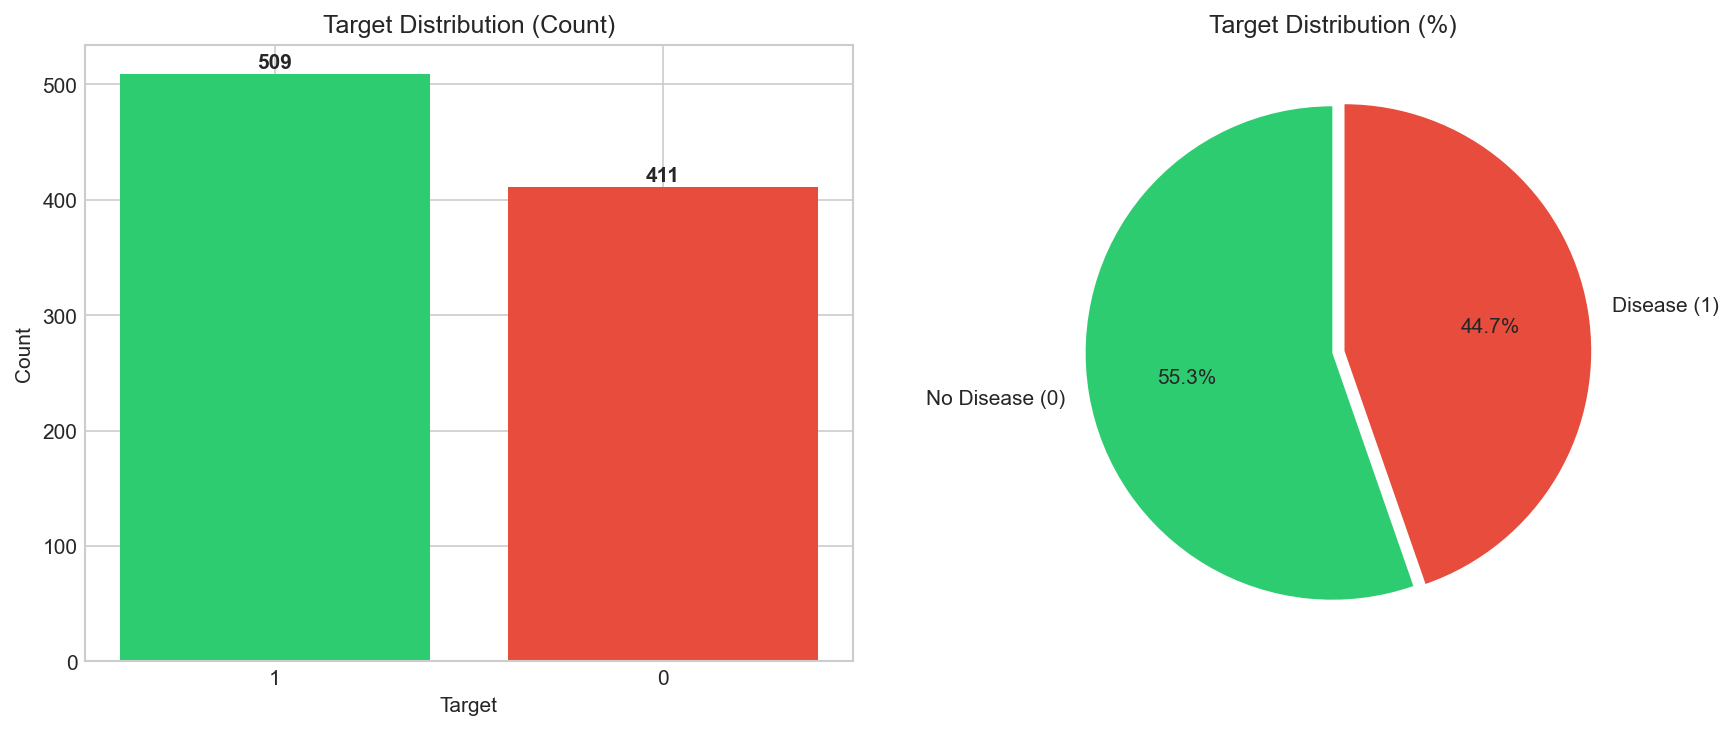
\includegraphics[width=0.7\textwidth]{figs/target_distribution.png}
    \caption{Phân bố biến mục tiêu (Target Distribution): 0 = không bệnh tim, 1 = có bệnh tim.}
    \label{fig:target_dist}
\end{figure}

\subsection{Thống kê mô tả và phân bố dữ liệu}

Hình \ref{fig:numeric_dist} trình bày phân bố histogram của các biến số liên tục trong tập dữ liệu. Qua phân tích, nhóm rút ra một số quan sát đáng chú ý:

\begin{itemize}
    \item \textbf{Tuổi (age):} Phân bố gần dạng chuẩn, tập trung trong khoảng 40--65 tuổi, trung vị khoảng 54 tuổi. Phần đuôi trái (dưới 30 tuổi) rất ít mẫu, cho thấy bệnh tim ít gặp ở nhóm trẻ tuổi, phù hợp với kiến thức y khoa.
    \item \textbf{Huyết áp lúc nghỉ (trestbps):} Phần lớn giá trị nằm trong khoảng 120--140 mmHg (huyết áp bình thường đến tăng huyết áp nhẹ). Có một số giá trị ngoại lai vượt 180 mmHg (tăng huyết áp nặng) và thậm chí giá trị 0 mmHg (rõ ràng là lỗi dữ liệu, cần xử lý).
    \item \textbf{Cholesterol huyết thanh (chol):} Phân bố lệch phải (right-skewed), trung bình khoảng 200--250 mg/dl. Nhiều giá trị ngoại lai phía trên 400 mg/dl, có cả giá trị 0 (có thể do missing hoặc lỗi đo). Cholesterol $\geq$ 240 mg/dl được coi là mức nguy hiểm theo tiêu chuẩn y khoa.
    \item \textbf{Nhịp tim tối đa (thalch):} Phân bố gần chuẩn, trung bình khoảng 137 bpm, dao động từ 60 đến 200 bpm. Bệnh nhân có nhịp tim tối đa thấp (không đạt được nhịp tim mục tiêu khi gắng sức) thường có nguy cơ bệnh tim cao hơn.
    \item \textbf{ST depression (oldpeak):} Phân bố lệch phải rất mạnh, đa số giá trị nằm trong khoảng 0--2 mm. Giá trị $\geq$ 2 mm thường có ý nghĩa bệnh lý và là dấu hiệu quan trọng của thiếu máu cơ tim.
\end{itemize}

\begin{figure}[H]
    \centering
    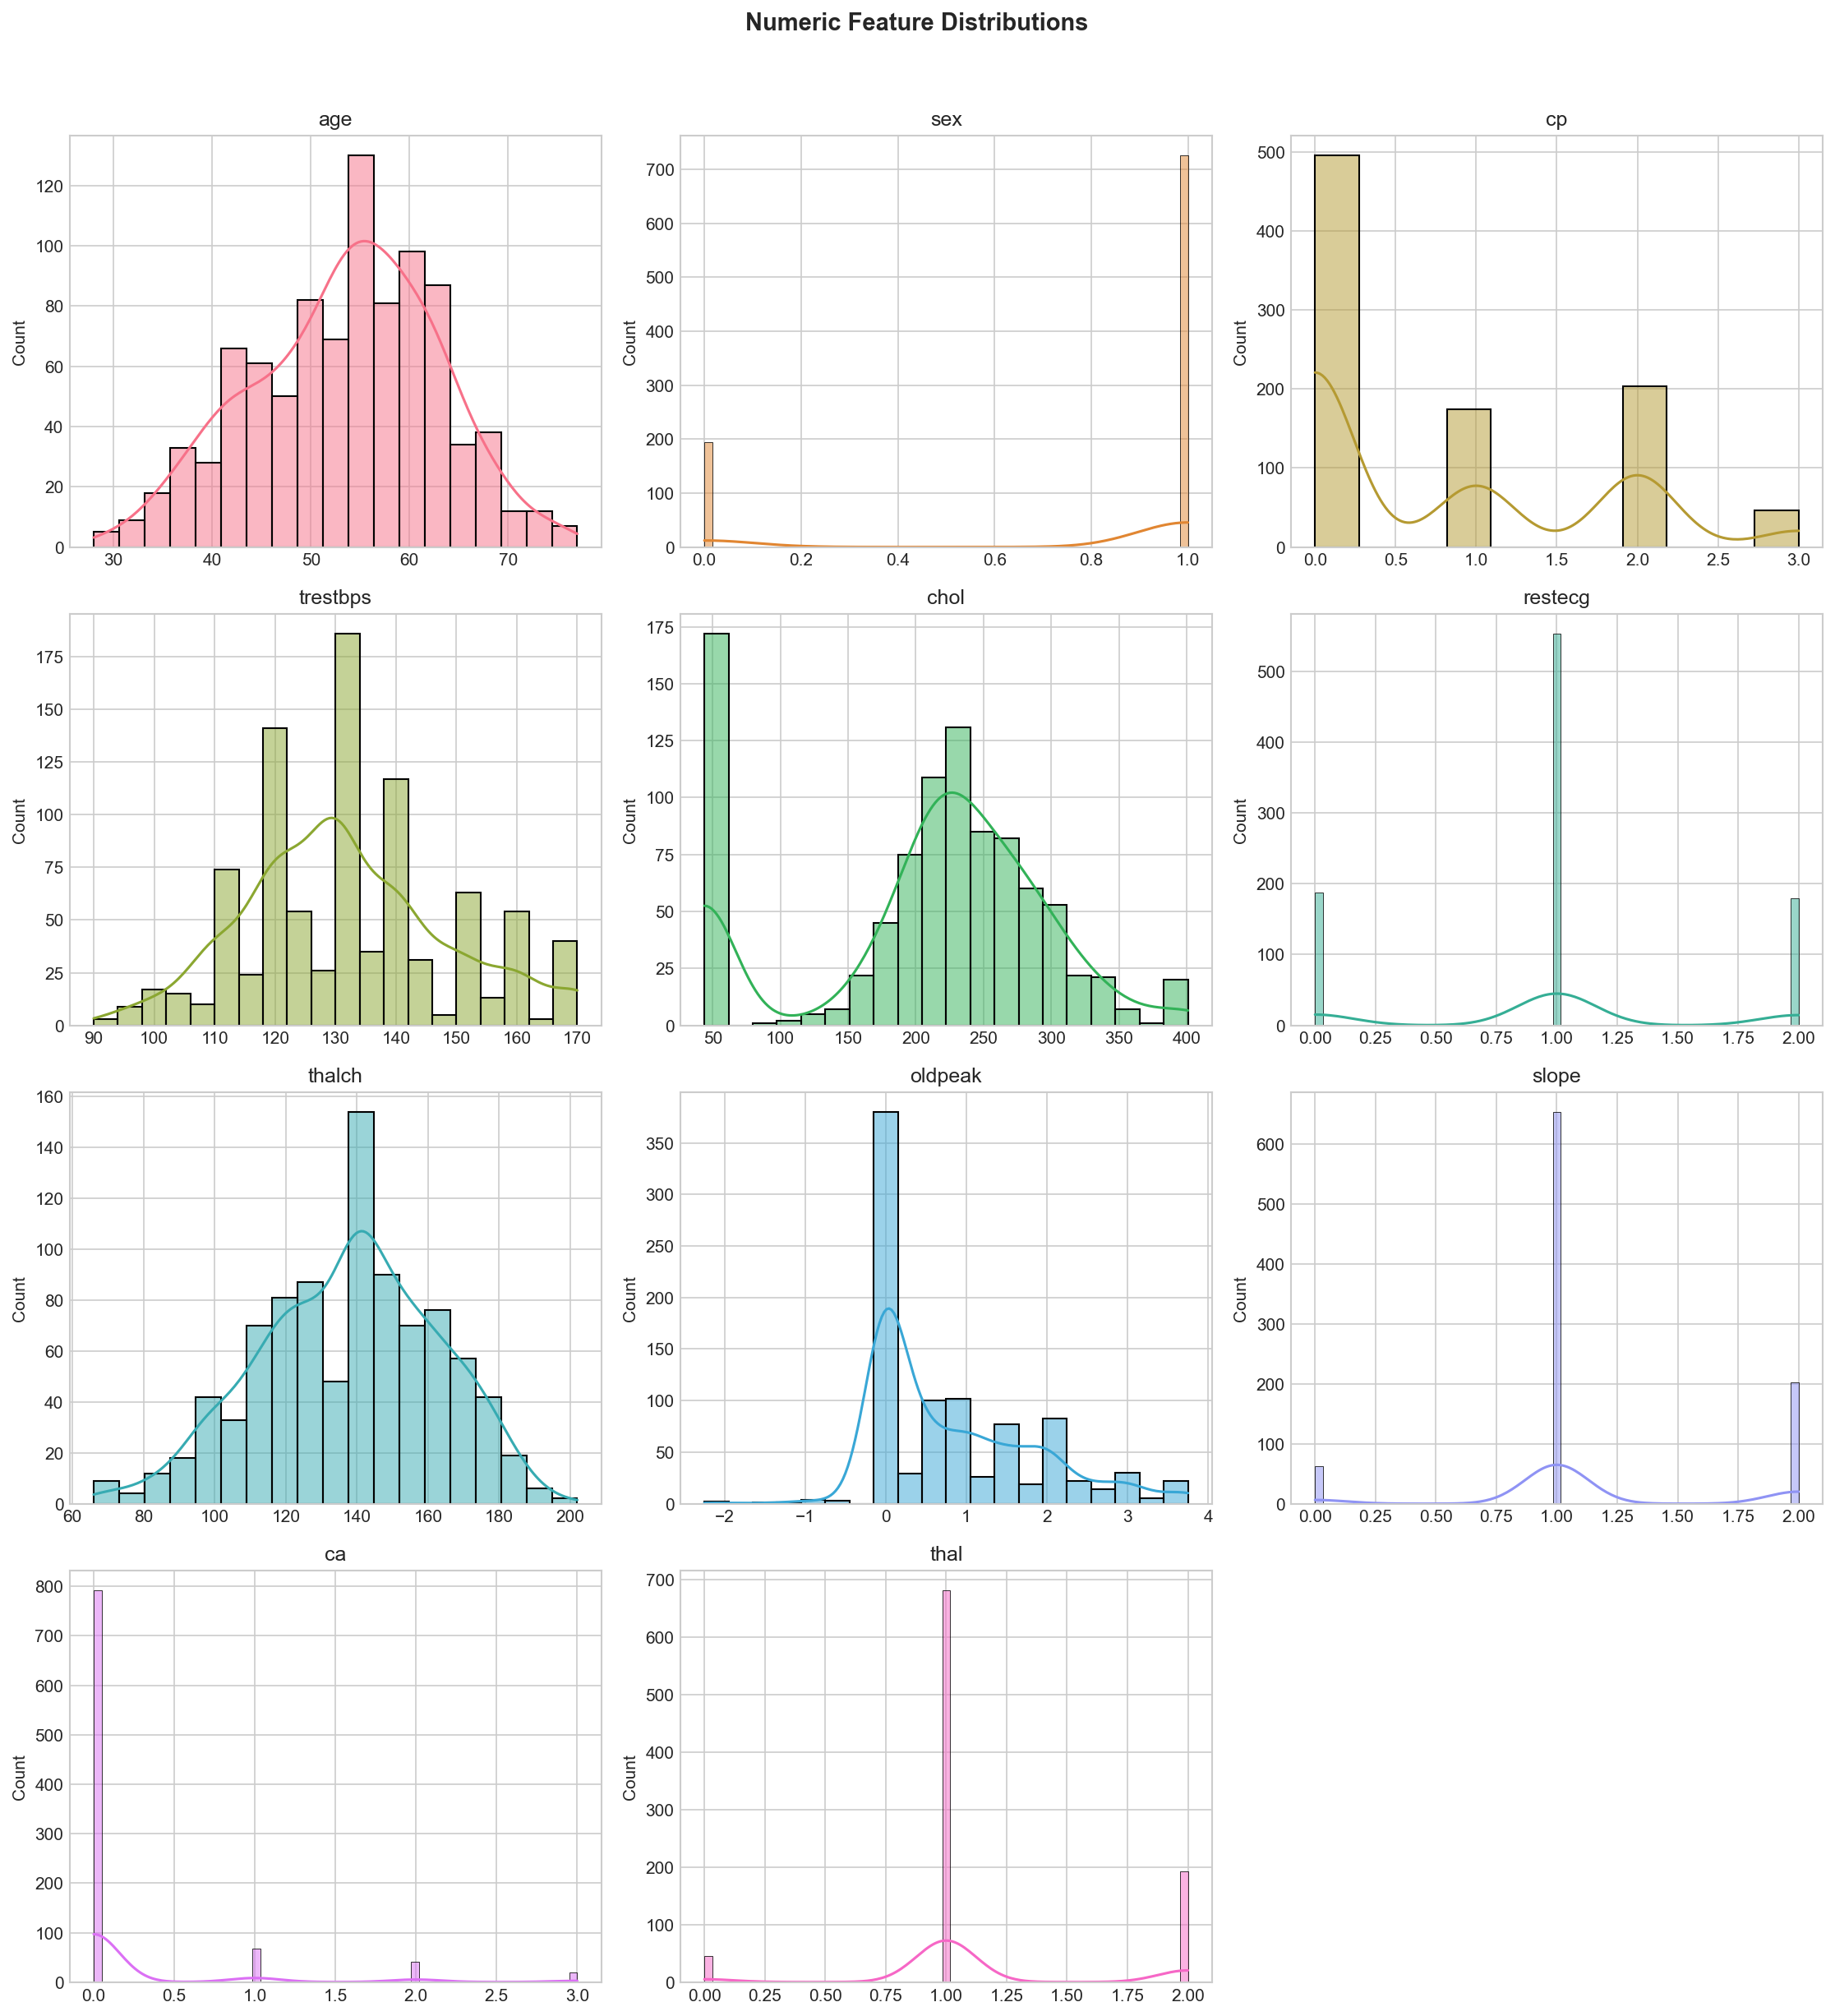
\includegraphics[width=\textwidth]{figs/numeric_distributions.png}
    \caption{Phân bố các biến số liên tục trong tập dữ liệu Heart Disease.}
    \label{fig:numeric_dist}
\end{figure}

\subsection{Tương quan giữa các biến}

Ma trận tương quan Pearson (Hình \ref{fig:corr_matrix}) thể hiện mối quan hệ tuyến tính giữa các biến số. Phân tích cho thấy:

\begin{itemize}
    \item \textbf{Tương quan dương mạnh nhất với target (bệnh tim):} Biến \texttt{oldpeak} (ST depression) và \texttt{ca} (số mạch nhuộm) có tương quan dương với biến mục tiêu, cho thấy bệnh nhân có giá trị cao ở hai biến này thường được chẩn đoán bệnh tim. Đây là hai chỉ số quan trọng trong chẩn đoán lâm sàng bệnh mạch vành.
    \item \textbf{Tương quan âm mạnh nhất với target:} Biến \texttt{thalch} (nhịp tim tối đa) có tương quan âm, nghĩa là bệnh nhân có nhịp tim tối đa thấp (tim không đáp ứng tốt khi gắng sức) thường có nguy cơ bệnh tim cao hơn.
    \item \textbf{Tương quan giữa các đặc trưng:} \texttt{thalch} và \texttt{age} có tương quan âm trung bình (tuổi càng cao thì nhịp tim tối đa khi gắng sức càng giảm -- phù hợp với sinh lý học). \texttt{oldpeak} và \texttt{age} có tương quan dương nhẹ (người lớn tuổi có xu hướng ST depression cao hơn).
    \item \textbf{Multicollinearity:} Không có cặp biến nào có tương quan quá cao ($|r| > 0.8$), cho thấy không cần loại bỏ biến do multicollinearity.
\end{itemize}

\begin{figure}[H]
    \centering
    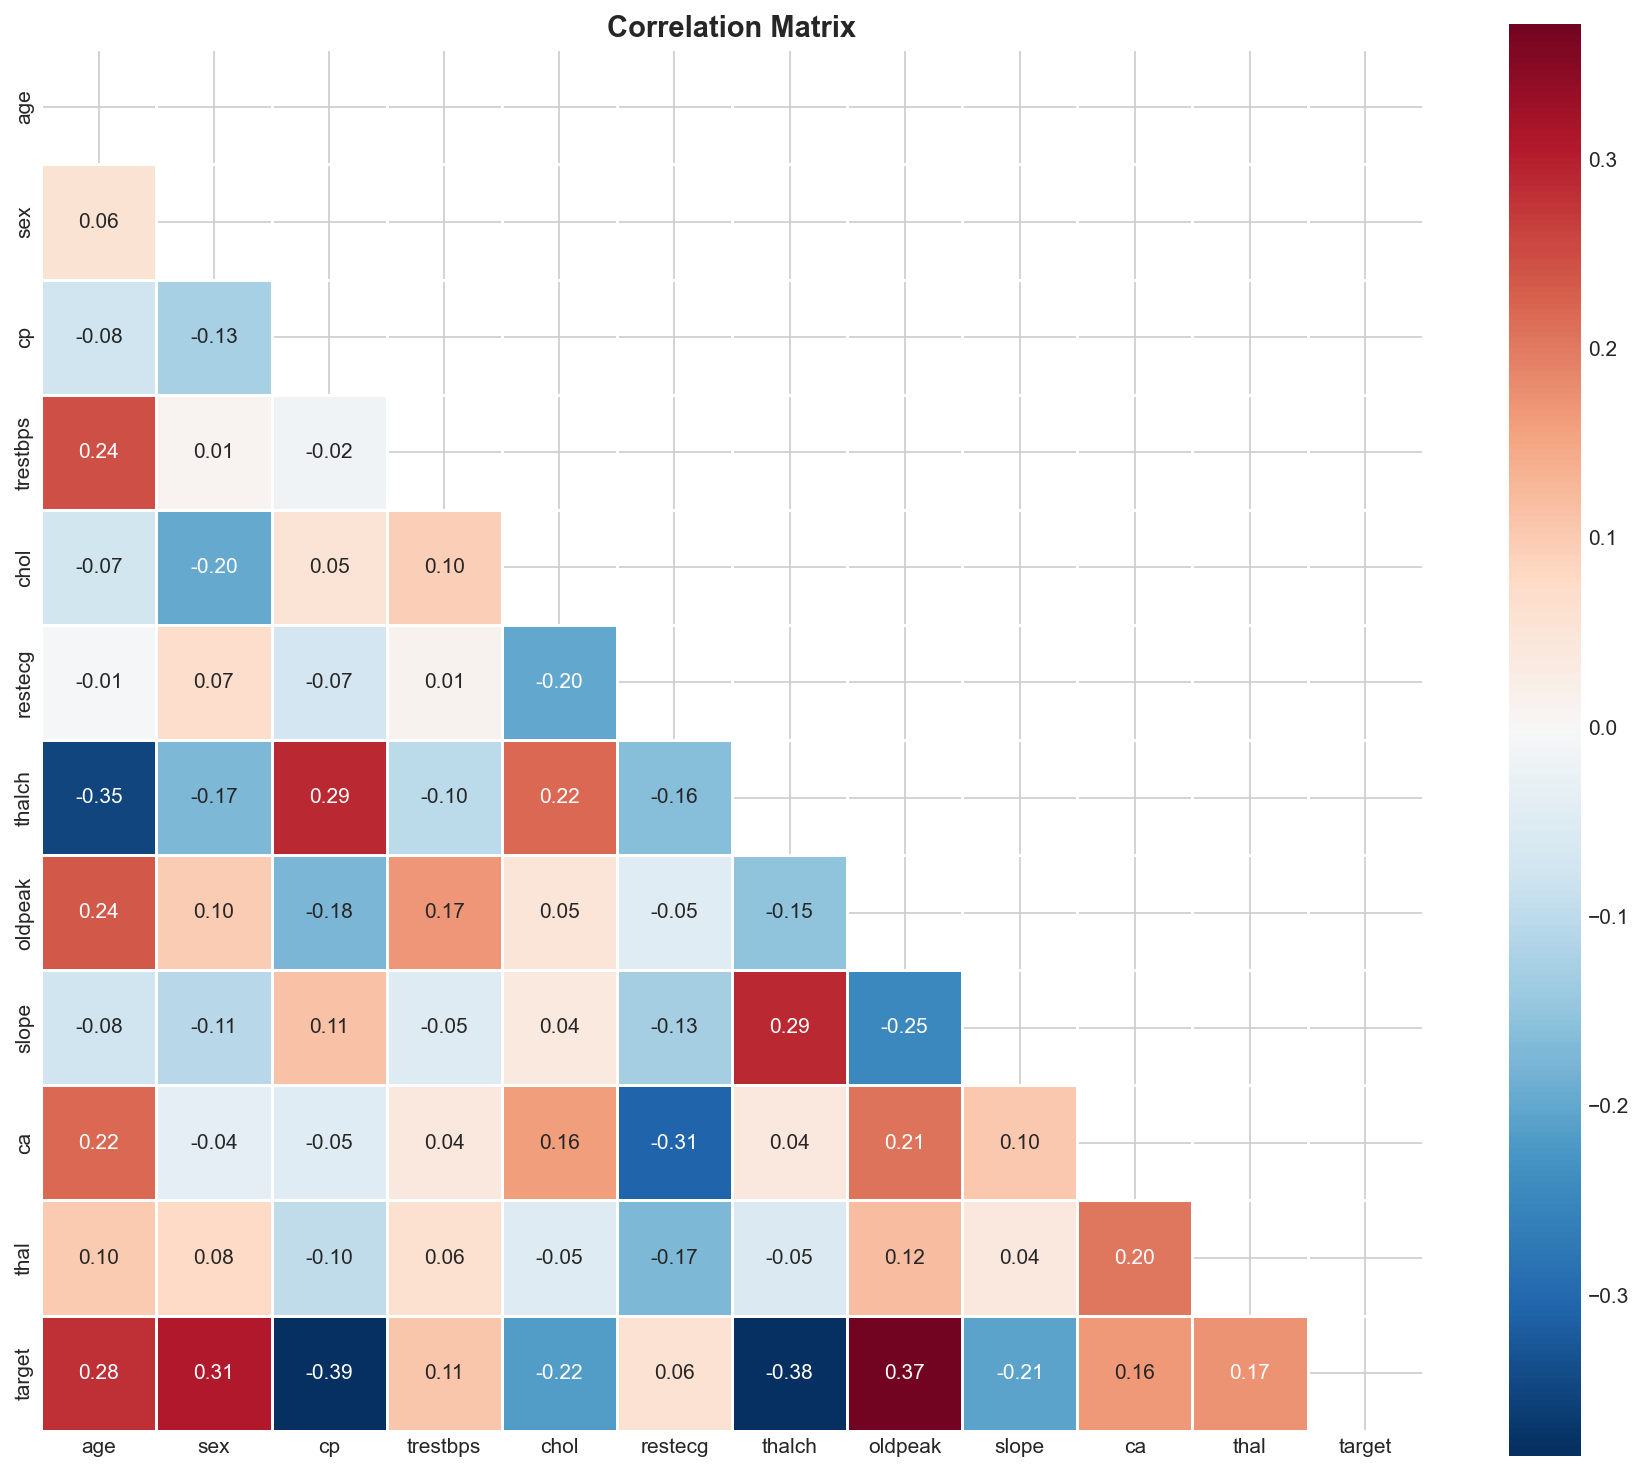
\includegraphics[width=0.85\textwidth]{figs/correlation_matrix.png}
    \caption{Ma trận tương quan Pearson giữa các biến số trong tập dữ liệu.}
    \label{fig:corr_matrix}
\end{figure}

Hình \ref{fig:features_target} minh họa chi tiết hơn mối quan hệ giữa các đặc trưng chính và biến mục tiêu, phân tách theo hai nhóm ``có bệnh'' và ``không bệnh''. Biểu đồ cho thấy sự khác biệt rõ rệt trong phân bố các đặc trưng giữa hai nhóm bệnh nhân, xác nhận rằng các features được chọn có khả năng phân biệt hai lớp.

\begin{figure}[H]
    \centering
    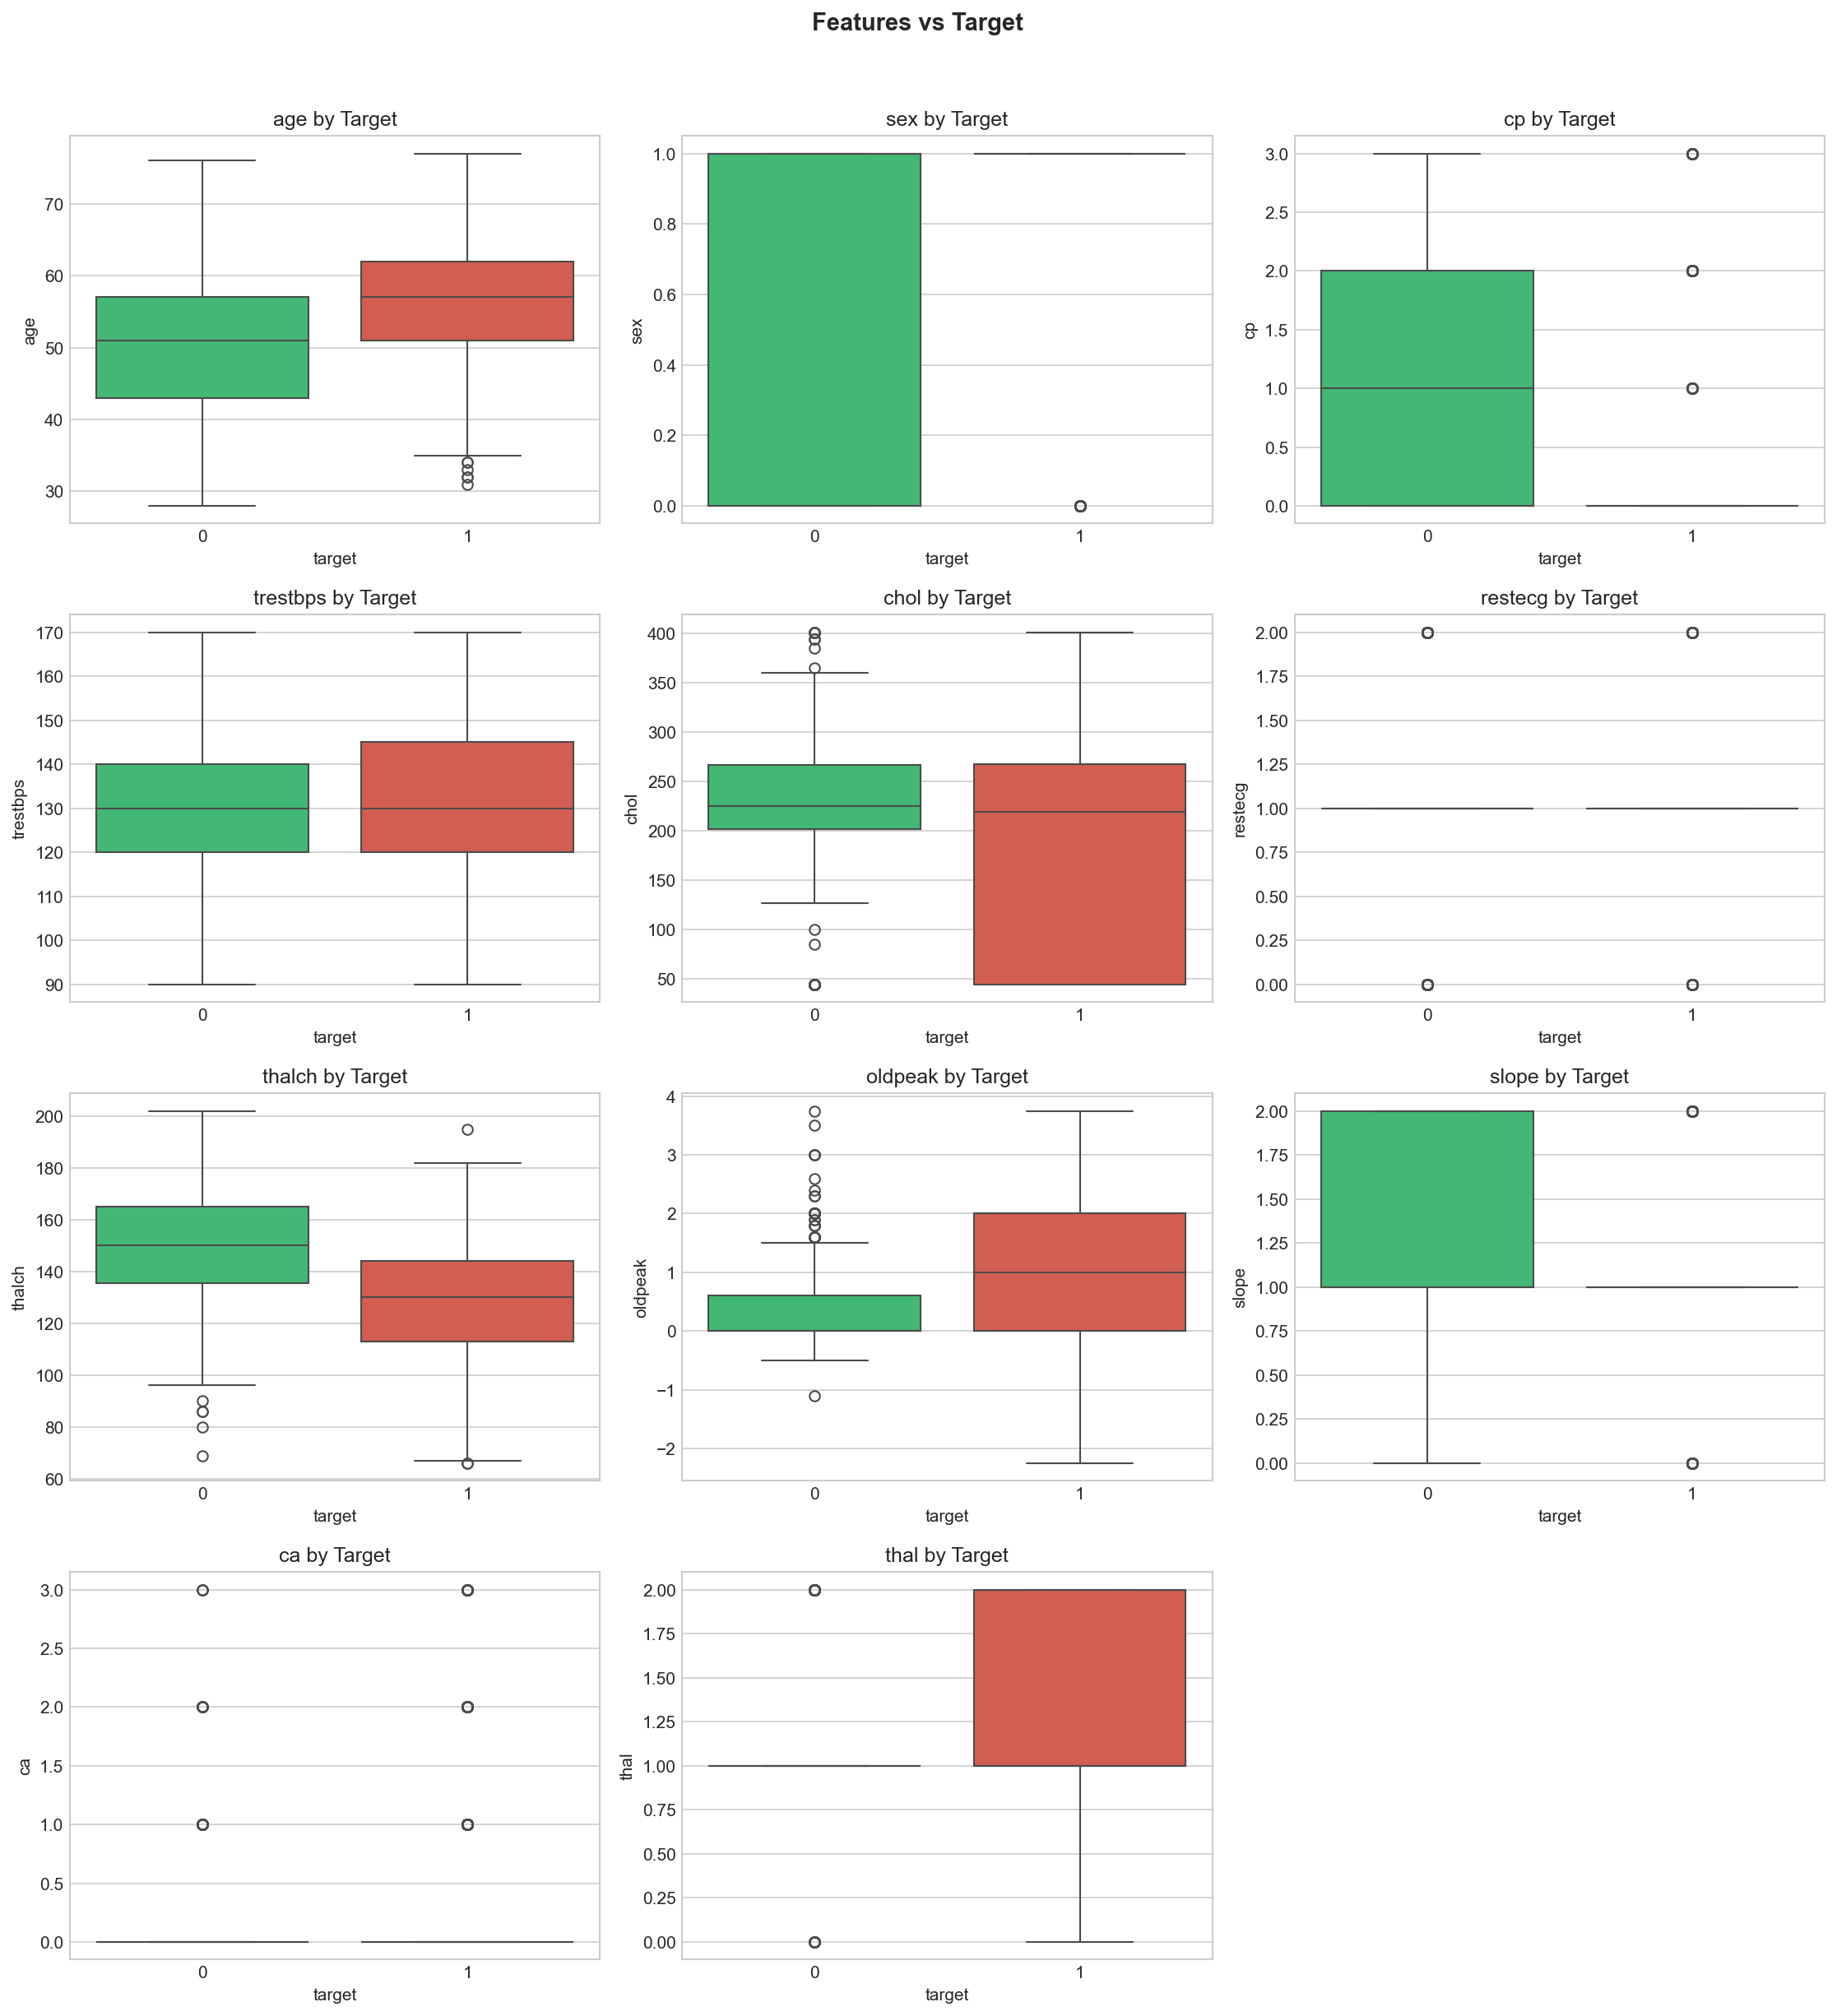
\includegraphics[width=\textwidth]{figs/features_vs_target.png}
    \caption{Phân bố các đặc trưng chính theo biến mục tiêu (0 vs 1).}
    \label{fig:features_target}
\end{figure}

\subsection{Phân tích dữ liệu thiếu (Missing Values)}

Chất lượng dữ liệu là yếu tố then chốt ảnh hưởng đến hiệu quả mô hình. Tập dữ liệu có tổng cộng \textbf{1.759 giá trị thiếu}, phân bố không đều giữa các cột. Hình \ref{fig:missing_values} cho thấy tỷ lệ missing values theo từng cột:

\begin{itemize}
    \item \texttt{ca} (số mạch nhuộm fluoroscopy): $\sim$65\% dữ liệu bị thiếu -- đây là cột có tỷ lệ missing cao nhất. Lý do: xét nghiệm fluoroscopy là phương pháp xâm lấn, tốn kém, không phải bệnh nhân nào cũng được thực hiện.
    \item \texttt{thal} (thalassemia): $\sim$53\% dữ liệu bị thiếu. Tương tự, xét nghiệm thalassemia không phải lúc nào cũng có sẵn ở tất cả các trung tâm y tế.
    \item \texttt{slope} (độ dốc đoạn ST): $\sim$33\% dữ liệu bị thiếu. Chỉ số này cần test gắng sức hoàn chỉnh, một số bệnh nhân không thể hoàn thành test.
    \item \texttt{fbs}, \texttt{restecg}, \texttt{exang}: tỷ lệ missing thấp hơn ($< 15\%$).
    \item \texttt{age}, \texttt{sex}, \texttt{cp}, \texttt{trestbps}: gần như không có missing.
\end{itemize}

\begin{figure}[H]
    \centering
    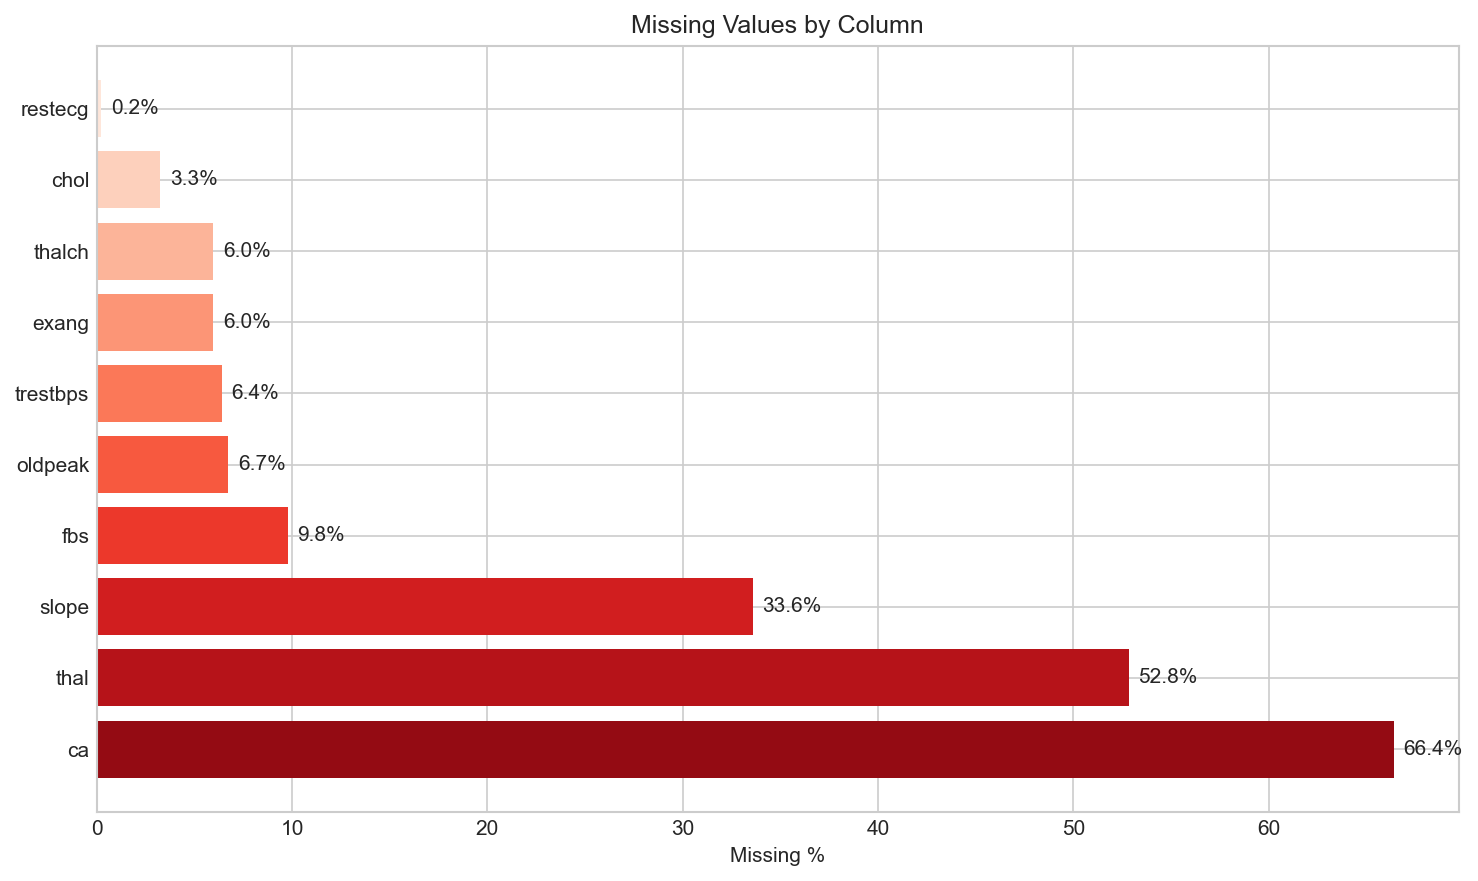
\includegraphics[width=0.8\textwidth]{figs/missing_values.png}
    \caption{Tỷ lệ dữ liệu thiếu (missing values) theo từng cột -- cột \texttt{ca} và \texttt{thal} có tỷ lệ thiếu rất cao.}
    \label{fig:missing_values}
\end{figure}

\subsection{Rủi ro và thách thức của dữ liệu}

Qua toàn bộ quá trình phân tích khám phá, nhóm nhận diện 5 rủi ro và thách thức chính cần xử lý:

\begin{enumerate}
    \item \textbf{Missing values cao ở các biến quan trọng:} Cột \texttt{ca} và \texttt{thal} có tỷ lệ thiếu $>$ 50\%, nhưng đây lại là những đặc trưng y khoa quan trọng, có tương quan mạnh với bệnh tim. Nhóm cần cân nhắc giữa hai chiến lược: loại bỏ cột (mất thông tin) hoặc fill giá trị (thêm noise). Chiến lược fill median/mode được chọn để giữ tối đa thông tin.
    
    \item \textbf{Mất cân bằng lớp nhẹ:} Tỷ lệ 55:45 giữa hai lớp không quá nghiêm trọng, nhưng cần xử lý để tránh mô hình thiên vị. Nhóm sử dụng hai kỹ thuật bổ sung: SMOTE (tạo mẫu tổng hợp cho lớp thiểu số) và \texttt{class\_weight=balanced} (điều chỉnh trọng số lớp trong thuật toán).
    
    \item \textbf{Data leakage tiềm ẩn:} Một sai lầm phổ biến trong Data Science là áp dụng preprocessing (scaling, SMOTE) trên toàn bộ dataset trước khi chia train/test. Điều này dẫn đến data leakage -- thông tin từ tập test ``rò rỉ'' vào tập train, làm kết quả đánh giá trở nên lạc quan hơn thực tế. Nhóm đảm bảo: StandardScaler được fit trên train, transform trên test; SMOTE chỉ áp dụng trên train.
    
    \item \textbf{Dữ liệu đa nguồn:} Dữ liệu từ 4 trung tâm y tế ở 3 quốc gia khác nhau, mỗi nơi có quy trình thu thập, thiết bị đo lường và population demographics khác nhau. Điều này tạo ra selection bias và measurement bias tiềm ẩn. Cột \texttt{dataset} được loại bỏ trong modeling, nhưng bias vẫn có thể tồn tại ở mức ngầm.
    
    \item \textbf{Giá trị ngoại lai (Outliers):} Các biến cholesterol, huyết áp có giá trị ngoại lai đáng kể (bao gồm cả giá trị 0 -- có khả năng là lỗi dữ liệu). Nhóm sử dụng phương pháp IQR (Interquartile Range) để phát hiện và clip outliers, giữ nguyên kích thước mẫu thay vì loại bỏ hàng.
\end{enumerate}

\chapter{Thiết kế giải pháp và quy trình khai phá dữ liệu}\label{chapter_pipeline}

\section{Pipeline tổng thể của hệ thống}

Quy trình khai phá dữ liệu của dự án được thiết kế theo mô hình pipeline tuần tự, một kiến trúc phổ biến trong các dự án Data Science. Pipeline bao gồm 6 giai đoạn chính, mỗi giai đoạn thực hiện một chức năng cụ thể và tạo ra đầu ra phục vụ cho giai đoạn tiếp theo. Bảng \ref{tab:pipeline_steps} mô tả chi tiết từng bước:

\begin{table}[H]
\centering
\caption{Các bước trong pipeline khai phá dữ liệu.}
\label{tab:pipeline_steps}
\begin{tabular}{|c|l|p{5.5cm}|p{3.5cm}|}
\hline
\textbf{Bước} & \textbf{Giai đoạn} & \textbf{Mô tả chi tiết} & \textbf{Đầu ra} \\ \hline
1 & Thu thập dữ liệu & Tải UCI Heart Disease Dataset (920 mẫu, 16 cột) từ file CSV & DataFrame gốc \\ \hline
2 & Tiền xử lý & Xử lý missing values, outliers, encoding biến phân loại, tạo biến target nhị phân & DataFrame sạch \\ \hline
3 & Xây dựng đặc trưng & Rời rạc hóa cho Apriori, chọn features cho Classification, chia train/test & Dữ liệu sẵn sàng cho modeling \\ \hline
4 & Khai phá dữ liệu & Chạy Apriori (luật kết hợp), KMeans + Hierarchical (phân cụm), SVM/RF/XGBoost (phân lớp) & Luật, nhãn cụm, mô hình \\ \hline
5 & Học bán giám sát & Self-training, Label Spreading với các tỷ lệ nhãn 5--50\% & Learning curves \\ \hline
6 & Đánh giá tổng hợp & Tính metrics, so sánh mô hình, phân tích lỗi, tạo báo cáo & Bảng kết quả, biểu đồ \\ \hline
\end{tabular}
\end{table}

Thiết kế pipeline có nhiều ưu điểm quan trọng trong dự án khai phá dữ liệu. Thứ nhất, tính \textbf{module hóa}: mỗi bước được cài đặt dưới dạng module Python riêng biệt trong thư mục \texttt{src/}, giúp dễ dàng bảo trì, cập nhật và tái sử dụng mã nguồn. Thứ hai, tính \textbf{tái lập} (reproducibility): toàn bộ tham số được quản lý tập trung qua file \texttt{configs/params.yaml} với \texttt{random\_state = 42}, đảm bảo kết quả có thể tái tạo chính xác. Thứ ba, \textbf{tự động hóa}: pipeline có thể chạy hoàn toàn tự động thông qua script \texttt{scripts/run\_pipeline.py}, hoặc thực hiện theo từng bước qua các notebook Jupyter trong thư mục \texttt{notebooks/} để phục vụ phân tích và trình diễn.

\section{Các bước tiền xử lý dữ liệu}

Tiền xử lý dữ liệu (Data Preprocessing) là giai đoạn then chốt quyết định chất lượng mô hình. Nguyên tắc chung là ``Garbage in, garbage out'' -- nếu dữ liệu đầu vào có chất lượng kém, mô hình sẽ cho kết quả thiếu tin cậy bất kể thuật toán tốt đến đâu. Nhóm thực hiện 5 bước tiền xử lý tuần tự:

\subsection{Loại bỏ cột không cần thiết}

Bước đầu tiên là loại bỏ hai cột không mang ý nghĩa dự đoán: \texttt{id} (mã định danh bệnh nhân, chỉ là số thứ tự) và \texttt{dataset} (tên trung tâm y tế thu thập dữ liệu). Cột \texttt{dataset} mặc dù có thể chứa thông tin về bias giữa các nguồn, nhưng không nên được sử dụng làm feature vì nó không phản ánh đặc điểm lâm sàng của bệnh nhân. Trong thực tế triển khai, mô hình cần dự đoán cho bệnh nhân mới không thuộc bất kỳ nguồn dữ liệu nào trong tập huấn luyện.

\subsection{Xử lý missing values}

Dữ liệu gốc có tổng cộng 1.759 giá trị thiếu, phân bố không đều giữa các cột (như phân tích ở Chương 1). Nhóm xem xét ba chiến lược xử lý missing values và phân tích ưu điểm, nhược điểm của từng phương pháp:

\textbf{Chiến lược 1: Drop cột có tỷ lệ missing cao (drop\_high\_missing).} Loại bỏ các cột có tỷ lệ thiếu vượt ngưỡng (ví dụ $>$ 40\%). Ưu điểm: đơn giản, không thêm noise. Nhược điểm: mất đi thông tin quan trọng từ \texttt{ca} và \texttt{thal} -- hai features có giá trị y khoa cao.

\textbf{Chiến lược 2: Fill tất cả (fill\_all).} Điền giá trị missing bằng thống kê mô tả. Ưu điểm: giữ được tất cả features. Nhược điểm: giá trị fill có thể không phản ánh đúng thực tế của bệnh nhân.

\textbf{Chiến lược 3: Drop hàng có missing (drop\_rows).} Loại bỏ các bệnh nhân có bất kỳ giá trị missing nào. Ưu điểm: dữ liệu hoàn toàn ``sạch''. Nhược điểm: mất rất nhiều mẫu (có thể giảm từ 920 xuống dưới 300 mẫu).

Sau khi cân nhắc, nhóm chọn \textbf{Chiến lược 2 (fill\_all)} vì đảm bảo giữ nguyên kích thước mẫu (920 bệnh nhân) và bảo toàn tất cả 13 features. Quy tắc fill cụ thể:
\begin{itemize}
    \item \textbf{Biến số liên tục} (\texttt{trestbps}, \texttt{chol}, \texttt{thalch}, \texttt{oldpeak}, \texttt{ca}): điền bằng giá trị \textbf{trung vị (median)}. Trung vị được chọn thay vì trung bình (mean) vì ít bị ảnh hưởng bởi giá trị ngoại lai. Ví dụ: nếu cholesterol có một số mẫu $>$ 500 mg/dl, mean sẽ bị kéo lên cao bất thường, trong khi median vẫn phản ánh giá trị trung tâm hợp lý.
    \item \textbf{Biến phân loại} (\texttt{fbs}, \texttt{restecg}, \texttt{exang}, \texttt{slope}, \texttt{thal}): điền bằng giá trị \textbf{mode} (giá trị xuất hiện nhiều nhất). Đây là phương pháp đơn giản nhất cho biến categorical, giả định rằng giá trị phổ biến nhất là ước lượng tốt nhất khi không có thông tin cụ thể.
\end{itemize}

\subsection{Xử lý outliers (ngoại lai)}

Giá trị ngoại lai (outliers) là những quan sát nằm xa phần lớn dữ liệu, có thể do lỗi đo lường, lỗi nhập liệu hoặc phản ánh tình trạng bệnh lý đặc biệt. Nhóm sử dụng phương pháp \textbf{IQR (Interquartile Range)} -- một kỹ thuật phát hiện outliers phi tham số, robust với phân bố dữ liệu bất kỳ.

Quy trình xử lý outliers bằng IQR gồm 4 bước:
\begin{enumerate}
    \item Tính phân vị thứ nhất $Q_1$ (25\%) và phân vị thứ ba $Q_3$ (75\%) cho mỗi biến số liên tục.
    \item Tính range liên phân vị: $IQR = Q_3 - Q_1$.
    \item Xác định ngưỡng dưới $L = Q_1 - 1.5 \times IQR$ và ngưỡng trên $U = Q_3 + 1.5 \times IQR$. Giá trị ngoại lai là những quan sát $< L$ hoặc $> U$.
    \item \textbf{Xử lý:} Thay vì loại bỏ hàng (mất dữ liệu), nhóm áp dụng phương pháp \textbf{cắt (clipping)}: các giá trị $< L$ được gán bằng $L$, các giá trị $> U$ được gán bằng $U$. Phương pháp này giữ nguyên kích thước mẫu và vẫn giữ lại thông tin rằng bệnh nhân có giá trị ``cực đoan''.
\end{enumerate}

Hệ số 1.5 là giá trị tiêu chuẩn trong thống kê, được John Tukey đề xuất. Với dữ liệu phân bố chuẩn, ngưỡng này tương đương khoảng 2.7 lần độ lệch chuẩn, loại bỏ khoảng 0.7\% quan sát cực trị ở mỗi phía.

\subsection{Encoding dữ liệu categorical}

Các thuật toán Machine Learning yêu cầu đầu vào dạng số, do đó các biến phân loại (categorical) cần được mã hóa (encoding). Nhóm xem xét hai phương pháp encoding phổ biến:

\textbf{Label Encoding:} Gán mỗi giá trị categorical một số nguyên. Ví dụ: \texttt{cp} với 4 giá trị $\rightarrow$ \{0, 1, 2, 3\}. Ưu điểm: giữ nguyên số chiều dữ liệu, đơn giản, nhanh. Nhược điểm: tạo ra thứ tự giả (ordinal relationship) giữa các giá trị, có thể gây hiểu sai cho một số thuật toán.

\textbf{One-hot Encoding:} Tạo một cột binary cho mỗi giá trị categorical. Ví dụ: \texttt{cp} với 4 giá trị $\rightarrow$ 4 cột binary (cp\_typical, cp\_atypical, cp\_nonanginal, cp\_asymptomatic). Ưu điểm: không tạo thứ tự giả. Nhược điểm: tăng đáng kể số chiều dữ liệu, đặc biệt khi biến có nhiều giá trị.

Nhóm chọn \textbf{Label Encoding} vì tập dữ liệu có kích thước trung bình (920 mẫu). Với One-hot Encoding, số features có thể tăng từ 13 lên 25--30 cột, dẫn đến curse of dimensionality khi số mẫu không đủ lớn. Hơn nữa, các thuật toán tree-based (Random Forest, XGBoost) xử lý tốt Label Encoding vì chúng tách (split) trên từng giá trị cụ thể, không bị ảnh hưởng bởi thứ tự giả.

Bảy biến categorical được encode: \texttt{sex}, \texttt{cp}, \texttt{fbs}, \texttt{restecg}, \texttt{exang}, \texttt{slope}, \texttt{thal}. Mapping encode được lưu lại để phục vụ diễn giải kết quả.

\subsection{Chuẩn hóa dữ liệu (Normalization / Scaling)}

Các biến số liên tục trong dữ liệu có đơn vị và khoảng giá trị rất khác nhau: tuổi (29--77 năm), huyết áp (94--200 mmHg), cholesterol (85--564 mg/dl), nhịp tim (71--202 bpm), oldpeak (0.0--6.2). Sự chênh lệch scale này ảnh hưởng đến các thuật toán sử dụng khoảng cách hoặc gradient.

\textbf{StandardScaler} được sử dụng để chuẩn hóa dữ liệu về phân bố chuẩn tắc (mean = 0, standard deviation = 1). Công thức chuyển đổi:
\[
z = \frac{x - \mu}{\sigma}
\]
trong đó $x$ là giá trị gốc, $\mu$ là trung bình và $\sigma$ là độ lệch chuẩn của cột tương ứng (tính trên tập train).

StandardScaler đặc biệt quan trọng cho:
\begin{itemize}
    \item \textbf{SVM:} Thuật toán SVM tối ưu hóa margin giữa các support vectors, nhạy cảm với scale. Nếu không scale, biến có range lớn (cholesterol) sẽ dominate biến có range nhỏ (oldpeak).
    \item \textbf{KMeans Clustering:} Sử dụng khoảng cách Euclidean để gán cụm. Nếu không scale, cụm sẽ bị chi phối bởi biến có range lớn nhất.
    \item \textbf{Logistic Regression:} Gradient descent hội tụ nhanh hơn khi các features ở cùng scale.
\end{itemize}

Random Forest và XGBoost ít nhạy cảm với scaling (vì sử dụng quyết định split), nhưng để đồng nhất và công bằng khi so sánh, tất cả mô hình đều nhận dữ liệu đã scale.

\textbf{Quy tắc chống data leakage:} Scaling được thực hiện \textbf{sau khi chia train/test}. Scaler được \texttt{fit()} trên tập train (học $\mu$ và $\sigma$), sau đó \texttt{transform()} trên cả tập train lẫn test. Điều này ngăn thông tin thống kê từ tập test ``rò rỉ'' vào quá trình training.

\subsection{Tạo biến mục tiêu nhị phân}

Cột \texttt{num} gốc có 5 mức: 0 (không bệnh), 1, 2, 3, 4 (các mức độ bệnh tim khác nhau, từ nhẹ đến nặng). Nhóm chuyển đổi thành biến nhị phân \texttt{target}:
\begin{itemize}
    \item $num = 0 \rightarrow target = 0$ (không bệnh tim)
    \item $num \in \{1, 2, 3, 4\} \rightarrow target = 1$ (có bệnh tim)
\end{itemize}

Lý do chọn binary thay vì multi-class: bài toán sàng lọc ban đầu cần trả lời câu hỏi ``có/không bệnh tim'', không cần phân biệt mức độ. Hơn nữa, phân bố các mức 1--4 rất mất cân bằng, gây khó khăn cho mô hình multi-class trên tập dữ liệu nhỏ.

\section{Xây dựng và lựa chọn đặc trưng (Feature Engineering)}

Feature Engineering là quá trình tạo ra hoặc biến đổi các đặc trưng để cải thiện hiệu quả mô hình. Trong dự án này, nhóm thực hiện hai hướng Feature Engineering khác nhau cho hai mục đích: rời rạc hóa phục vụ thuật toán Apriori, và chọn features phục vụ mô hình phân lớp.

\subsection{Rời rạc hóa cho thuật toán Apriori}

Thuật toán Apriori yêu cầu đầu vào dạng giao dịch nhị phân (transaction: mỗi bản ghi là tập hợp các items xuất hiện/không xuất hiện). Do đó, tất cả biến liên tục và phân loại cần được chuyển đổi thành dạng binary (0/1). Nhóm thực hiện rời rạc hóa (discretization) dựa trên \textbf{ngưỡng y khoa} (medical thresholds) -- các giá trị phân loại được công nhận trong y văn:

\begin{table}[H]
\centering
\caption{Quy tắc rời rạc hóa các biến liên tục theo ngưỡng y khoa.}
\label{tab:discretization}
\small
\begin{tabular}{|l|l|p{4.5cm}|p{3cm}|}
\hline
\textbf{Biến gốc} & \textbf{Biến binary} & \textbf{Ngưỡng} & \textbf{Cơ sở y khoa} \\ \hline
\texttt{age} & \texttt{age\_young}, \texttt{age\_middle}, \texttt{age\_senior}, \texttt{age\_elderly} & $<$40, 40--54, 55--64, $\geq$65 (tuổi) & Nhóm tuổi theo nguy cơ tim mạch \\ \hline
\texttt{trestbps} & \texttt{bp\_normal}, \texttt{bp\_elevated}, \texttt{bp\_high} & $<$120, 120--139, $\geq$140 (mmHg) & Phân loại huyết áp WHO \\ \hline
\texttt{chol} & \texttt{chol\_normal}, \texttt{chol\_borderline}, \texttt{chol\_high} & $<$200, 200--239, $\geq$240 (mg/dl) & Tiêu chuẩn ATP III \\ \hline
\texttt{thalch} & \texttt{hr\_low}, \texttt{hr\_normal}, \texttt{hr\_high} & $<$120, 120--159, $\geq$160 (bpm) & Ngưỡng lâm sàng \\ \hline
\texttt{oldpeak} & \texttt{oldpeak\_zero}, \texttt{oldpeak\_low}, \texttt{oldpeak\_high} & $=0$, $0$--$2$, $\geq 2$ (mm) & ST depression $\geq$2mm có ý nghĩa bệnh lý \\ \hline
\texttt{ca} & \texttt{ca\_zero}, \texttt{ca\_positive} & $= 0$, $> 0$ & Mạch nhuộm fluoroscopy \\ \hline
\end{tabular}
\end{table}

Việc sử dụng ngưỡng y khoa thay vì ngưỡng thống kê (quantile-based) có hai ưu điểm quan trọng. Thứ nhất, kết quả luật kết hợp có thể diễn giải trực tiếp trong ngữ cảnh y tế (ví dụ: ``cholesterol\_high'' dễ hiểu hơn ``cholesterol\_Q4''). Thứ hai, ngưỡng không phụ thuộc vào phân bố của tập dữ liệu cụ thể, tăng tính tổng quát hóa. Các biến phân loại gốc (\texttt{sex}, \texttt{cp}, \texttt{fbs}, \texttt{restecg}, \texttt{exang}, \texttt{slope}, \texttt{thal}) cũng được chuyển đổi tương tự thành dạng binary, tạo ra tổng cộng khoảng 25--30 biến binary cho Apriori.

\subsection{Lựa chọn đặc trưng cho mô hình phân lớp}

Đối với các mô hình phân lớp (SVM, Random Forest, XGBoost), nhóm sử dụng tất cả 13 features sau khi loại bỏ cột \texttt{id} và \texttt{dataset}. Quyết định giữ toàn bộ features (thay vì feature selection) dựa trên hai lý do: (1) số chiều hiện tại (13) không quá cao so với số mẫu (920), chưa gặp curse of dimensionality; (2) Random Forest và XGBoost có cơ chế feature importance nội tại, tự ``chọn'' features quan trọng trong quá trình training mà không cần loại bỏ thủ công.

Hàm \texttt{select\_features\_for\_modeling()} chuẩn bị dữ liệu bằng cách tách DataFrame thành ma trận đặc trưng $X$ (13 cột) và vector nhãn $y$ (cột \texttt{target}).

\section{Lựa chọn mô hình và thuật toán}

\subsection{Luật kết hợp -- Thuật toán Apriori}

Thuật toán \textbf{Apriori} \cite{agrawal1994fast} là một trong những thuật toán kinh điển nhất trong khai phá dữ liệu, được thiết kế để tìm frequent itemsets (tập mẫu phổ biến) và sinh luật kết hợp (association rules) từ dữ liệu giao dịch. Thuật toán hoạt động theo nguyên lý ``anti-monotone'': nếu một tập mẫu không phổ biến (support $<$ min\_support), thì tất cả các tập mẫu chứa nó cũng không phổ biến. Nguyên lý này giúp cắt tỉa (pruning) không gian tìm kiếm hiệu quả.

Tham số cấu hình được chọn sau quá trình thử nghiệm:
\begin{itemize}
    \item \texttt{min\_support} = 0.08: Tập mẫu phải xuất hiện trong ít nhất 8\% dataset ($\approx$ 74 bệnh nhân). Ngưỡng này đủ thấp để tìm được các tổ hợp triệu chứng hiếm nhưng quan trọng, đồng thời đủ cao để loại bỏ các tổ hợp quá hiếm không có ý nghĩa thống kê.
    \item \texttt{min\_confidence} = 0.50: Ít nhất 50\% trường hợp thỏa mãn điều kiện thì kết luận đúng. Trong y tế, confidence $>$ 0.80 được coi là luật mạnh.
    \item \texttt{min\_lift} = 1.2: Nguy cơ cao hơn ít nhất 1.2 lần so với ngẫu nhiên. Lift = 1.0 nghĩa là không có mối liên hệ; lift $>$ 1.0 cho thấy tương quan dương.
\end{itemize}

\subsection{Phân cụm -- KMeans và Hierarchical Clustering}

Hai thuật toán phân cụm được triển khai để cung cấp cái nhìn bổ sung cho nhau:

\textbf{KMeans} \cite{lloyd1982least} là thuật toán phân cụm dựa trên prototype, chia $n$ điểm dữ liệu thành $k$ cụm bằng cách tối thiểu hóa tổng khoảng cách Euclidean bình phương từ mỗi điểm đến centroid cụm gần nhất. Nhóm xác định số cụm tối ưu bằng hai phương pháp bổ sung: (1) \textbf{Elbow method}: vẽ đồ thị inertia (tổng khoảng cách trong cụm) theo $k$, tìm điểm ``khuỷu tay'' nơi tốc độ giảm inertia chậm lại đáng kể; (2) \textbf{Silhouette Score}: đánh giá mức độ tách biệt giữa các cụm, chọn $k$ có Silhouette Score cao nhất. Tham số \texttt{n\_init = 10} được sử dụng để chạy KMeans 10 lần với các centroid khởi tạo ngẫu nhiên khác nhau, chọn kết quả tốt nhất.

\textbf{Hierarchical Clustering (Agglomerative)} xây dựng cây phân cấp (dendrogram) bằng cách gộp hai cụm gần nhất tại mỗi bước. Phương pháp linkage \textbf{Ward} được chọn vì tối thiểu hóa tổng variance nội cụm, thường cho kết quả compact và cân bằng nhất. So với KMeans, Hierarchical Clustering cung cấp thông tin về cấu trúc phân cấp của dữ liệu, giúp hiểu mối quan hệ giữa các nhóm bệnh nhân ở nhiều mức granularity khác nhau.

\subsection{Phân lớp -- SVM, Random Forest, XGBoost}

Nhóm triển khai 6 mô hình phân lớp (2 baseline + 4 cải tiến), đảm bảo đánh giá công bằng và toàn diện:

\begin{table}[H]
\centering
\caption{Các mô hình phân lớp và tham số chính cùng lý do lựa chọn.}
\label{tab:models}
\small
\begin{tabular}{|l|p{5cm}|p{5cm}|}
\hline
\textbf{Mô hình} & \textbf{Tham số chính} & \textbf{Lý do lựa chọn} \\ \hline
Baseline (Dummy) & strategy = most\_frequent & Đường cơ sở, dự đoán lớp đa số \\ \hline
Baseline (Logistic) & max\_iter=1000, class\_weight=balanced & Baseline mạnh, nhanh, dễ diễn giải \\ \hline
SVM (linear) \cite{cortes1995support} & kernel=linear, probability=True, class\_weight=balanced & Xử lý high-dimensional data, margin tối ưu \\ \hline
SVM (RBF) \cite{cortes1995support} & kernel=rbf, probability=True, class\_weight=balanced & Xử lý non-linearly separable data qua kernel trick \\ \hline
Random Forest \cite{breiman2001random} & n\_estimators=200, max\_depth=10, class\_weight=balanced & Ensemble bagging, robust với noise và outliers \\ \hline
XGBoost \cite{chen2016xgboost} & n\_estimators=200, max\_depth=5, learning\_rate=0.1, eval\_metric=logloss & State-of-the-art gradient boosting cho tabular data \\ \hline
\end{tabular}
\end{table}

Tham số \texttt{class\_weight=balanced} (SVM, RF, Logistic) tự động điều chỉnh trọng số mất mát cho mỗi lớp theo tỷ lệ nghịch với số mẫu. Với dữ liệu 55:45, lớp thiểu số (không bệnh) được tăng trọng số, giúp mô hình chú ý hơn đến lớp này. SMOTE (Synthetic Minority Over-sampling Technique) \cite{chawla2002smote} được áp dụng bổ sung trên tập train, tạo mẫu tổng hợp cho lớp thiểu số bằng cách interpolation giữa các mẫu gần nhau trong không gian đặc trưng.

\subsection{Học bán giám sát -- Self-training và Label Spreading}

Trong thực tế y tế, dữ liệu có nhãn chẩn đoán thường đắt đỏ (cần bác sĩ chuyên khoa xác nhận) trong khi dữ liệu chưa gán nhãn rất phong phú. Học bán giám sát \cite{chapelle2006semi} khai thác cả dữ liệu có nhãn lẫn không nhãn để cải thiện mô hình.

\textbf{Self-training} là phương pháp wrapper đơn giản: (1) Train mô hình cơ sở (SVM) trên dữ liệu có nhãn; (2) Dùng mô hình dự đoán nhãn (pseudo-labels) cho dữ liệu chưa gán nhãn; (3) Chọn các pseudo-labels có confidence cao ($>$ ngưỡng), thêm vào tập train; (4) Lặp lại cho đến khi hội tụ. Ưu điểm: đơn giản, có thể dùng với bất kỳ classifier nào.

\textbf{Label Spreading} \cite{zhou2004learning} là phương pháp graph-based: xây dựng đồ thị similarity giữa các mẫu, sau đó lan truyền nhãn từ labeled nodes sang unlabeled nodes dựa trên trọng số cạnh. Phương pháp này mạnh khi dữ liệu có cấu trúc manifold rõ ràng.

Nhóm thử nghiệm với 6 tỷ lệ nhãn: 5\%, 10\%, 15\%, 20\%, 30\%, 50\%. Ở mỗi tỷ lệ, chỉ giữ lại $r\%$ nhãn gốc (chọn ngẫu nhiên, stratified), phần còn lại đặt nhãn = $-1$ (unlabeled). So sánh kết quả với supervised learning (chỉ train trên phần có nhãn) để đánh giá giá trị gia tăng của semi-supervised.

\section{Quy trình chia dữ liệu và cân bằng lớp}

\subsection{Chiến lược chia dữ liệu (Data Splitting)}

Chia dữ liệu là bước cực kỳ quan trọng trong Machine Learning, ảnh hưởng trực tiếp đến tính khách quan của đánh giá mô hình. Nhóm sử dụng chiến lược \textbf{Stratified Train/Test Split} với tỷ lệ 80/20, nghĩa là 80\% dữ liệu dùng để huấn luyện và 20\% còn lại dùng để đánh giá. Tham số \texttt{random\_state = 42} được sử dụng nhất quán trong toàn bộ dự án.

Phương pháp ``Stratified'' đảm bảo rằng tỷ lệ lớp mục tiêu (55\% bệnh vs 45\% không bệnh) được duy trì chính xác trong cả tập train (736 mẫu) và tập test (184 mẫu). Nếu sử dụng random split thông thường (không stratified), với tập dữ liệu chỉ 920 mẫu, tập test có thể bị lệch đáng kể -- ví dụ 60:40 thay vì 55:45 -- dẫn đến kết quả đánh giá thiên vị. Stratified split loại bỏ hoàn toàn nguồn sai số này.

Một nguyên tắc quan trọng được tuân thủ nghiêm ngặt: \textbf{tập test là ``holy'' -- không bao giờ được sử dụng trong quá trình training}. Cụ thể:
\begin{itemize}
    \item StandardScaler chỉ \texttt{fit()} trên tập train, sau đó \texttt{transform()} trên cả train và test. Nghĩa là $\mu$ và $\sigma$ được tính từ 736 mẫu train, không phải 920 mẫu.
    \item SMOTE chỉ tạo mẫu tổng hợp trên tập train. Mẫu synthetic không ảnh hưởng đến tập test.
    \item Feature selection, hyperparameter tuning (nếu có) chỉ dựa trên cross-validation trong tập train.
\end{itemize}

Việc vi phạm các nguyên tắc này sẽ dẫn đến \textbf{data leakage} -- một lỗi phổ biến nhưng nghiêm trọng trong Machine Learning, khiến mô hình ``gian lận'' bằng cách sử dụng thông tin từ tập test, tạo ra kết quả đánh giá lạc quan giả tạo (optimistic bias). Trong thực tế triển khai, mô hình sẽ thất bại khi gặp dữ liệu mới chưa từng thấy.

\subsection{Kỹ thuật SMOTE (Synthetic Minority Over-sampling)}

SMOTE \cite{chawla2002smote} là kỹ thuật cân bằng lớp phổ biến nhất trong Machine Learning, được thiết kế để xử lý vấn đề dữ liệu mất cân bằng. Trong bài toán dự đoán bệnh tim, tỷ lệ mất cân bằng 55:45 không quá nghiêm trọng, nhưng nhóm vẫn áp dụng SMOTE vì hai lý do: (1) cải thiện Recall cho lớp thiểu số, giảm False Negative -- quan trọng trong y tế; (2) giúp mô hình học decision boundary cân bằng hơn.

Quy trình hoạt động của SMOTE:
\begin{enumerate}
    \item Chọn một mẫu từ lớp thiểu số (minority class).
    \item Tìm $k$ nearest neighbors ($k = 5$ mặc định) của mẫu đó trong không gian đặc trưng, chỉ xét các mẫu cùng lớp thiểu số.
    \item Chọn ngẫu nhiên một trong $k$ neighbors.
    \item Tạo mẫu tổng hợp (synthetic sample) bằng phép nội suy (interpolation) tuyến tính: $x_{new} = x_{i} + \lambda \cdot (x_{nn} - x_{i})$, trong đó $\lambda \sim U(0,1)$.
    \item Lặp lại cho đến khi hai lớp cân bằng.
\end{enumerate}

Ưu điểm của SMOTE so với random oversampling (nhân bản mẫu): SMOTE tạo ra mẫu ``mới'' nằm giữa các mẫu thật, mở rộng vùng quyết định của lớp thiểu số mà không chỉ đơn thuần nhân bản (tránh overfitting trên cùng một mẫu lặp lại nhiều lần). Tuy nhiên, cần lưu ý rằng mẫu synthetic là ``nhân tạo'' -- không phải bệnh nhân thật -- nên có thể tạo ra mẫu ở vùng decision boundary không realistic.

\subsection{Tóm tắt luồng dữ liệu tổng thể}

Để cung cấp cái nhìn tổng hợp, luồng dữ liệu từ đầu đến cuối pipeline được tóm tắt:

$$\text{Raw CSV (920 $\times$ 16)} \xrightarrow{\text{drop id, dataset}} \text{(920 $\times$ 14)} \xrightarrow{\text{fill missing}} \text{(920 $\times$ 14, no null)}$$
$$\xrightarrow{\text{encode + outlier + binary target}} \text{Clean (920 $\times$ 14)} \xrightarrow{\text{split 80/20}} \text{Train (736) + Test (184)}$$
$$\text{Train} \xrightarrow{\text{scale + SMOTE}} \text{Train\_ready} \xrightarrow{\text{6 models}} \text{Predictions + Metrics}$$

Song song với pipeline phân lớp, nhánh Apriori hoạt động trên dữ liệu đã rời rạc hóa (before split), và nhánh phân cụm hoạt động trên dữ liệu đã scale (toàn bộ 920 mẫu). Nhánh semi-supervised hoạt động trên Train\_ready với các tỷ lệ nhãn khác nhau.

\chapter{Phân tích mã nguồn và chức năng hệ thống}\label{chapter_code}

\section{Tổng quan kiến trúc hệ thống}

Hệ thống dự đoán bệnh tim được phát triển bằng ngôn ngữ Python, tận dụng hệ sinh thái thư viện khoa học dữ liệu phong phú của Python bao gồm Pandas, NumPy, scikit-learn \cite{pedregosa2011scikit}, XGBoost, mlxtend và Matplotlib. Mã nguồn được quản lý trên GitHub, tuân theo các best practices trong phát triển dự án Data Science: quản lý phiên bản (version control), cấu trúc module hóa, tách biệt giữa code logic và notebook trình diễn, và quản lý tham số tập trung.

Kiến trúc tổng thể của dự án tuân theo mô hình \textbf{ba lớp} (three-tier architecture):
\begin{itemize}
    \item \textbf{Lớp trình diễn (Presentation Layer):} Các Jupyter notebooks (\texttt{notebooks/}) phục vụ phân tích tương tác và trình diễn kết quả; ứng dụng Streamlit (\texttt{app.py}) cung cấp giao diện web demo cho người dùng cuối.
    \item \textbf{Lớp logic nghiệp vụ (Business Logic Layer):} Các module Python trong thư mục \texttt{src/} chứa toàn bộ logic xử lý dữ liệu, xây dựng đặc trưng, huấn luyện mô hình và đánh giá. Các module này được thiết kế để tái sử dụng -- có thể gọi từ notebook, script hoặc ứng dụng web.
    \item \textbf{Lớp dữ liệu (Data Layer):} Thư mục \texttt{data/} chứa dữ liệu gốc và đã xử lý; \texttt{outputs/} chứa kết quả (mô hình, biểu đồ, bảng); \texttt{configs/} chứa tham số cấu hình.
\end{itemize}

Thiết kế ba lớp giúp phân tách rõ ràng giữa giao diện, logic và dữ liệu, tạo ra codebase dễ bảo trì, mở rộng và kiểm thử. Khi cần thay đổi thuật toán hoặc tham số, chỉ cần sửa ở lớp logic mà không ảnh hưởng đến giao diện; khi cần thay đổi dữ liệu đầu vào, chỉ cần cập nhật đường dẫn trong file cấu hình.

\section{Cấu trúc repository chi tiết}

Bảng \ref{tab:repo_structure} trình bày cấu trúc thư mục và file chính của dự án, cùng với vai trò cụ thể của từng thành phần:

\begin{table}[H]
\centering
\caption{Cấu trúc thư mục và vai trò trong dự án.}
\label{tab:repo_structure}
\small
\begin{tabular}{|l|p{9cm}|}
\hline
\textbf{Thư mục / File} & \textbf{Vai trò và mô tả chi tiết} \\ \hline
\texttt{configs/params.yaml} & File cấu hình tập trung dạng YAML, chứa: random seed (42), đường dẫn dữ liệu, tỷ lệ chia train/test (80/20), chiến lược xử lý missing, hyperparameters của Apriori, KMeans, Classification và Semi-supervised \\ \hline
\texttt{data/raw/heart.csv} & Dữ liệu gốc UCI Heart Disease (920 dòng $\times$ 16 cột), chưa qua bất kỳ xử lý nào \\ \hline
\texttt{data/processed/} & Dữ liệu sau tiền xử lý: \texttt{heart\_processed.csv} (clean), \texttt{heart\_discretized.csv} (binary cho Apriori) \\ \hline
\texttt{notebooks/} & 6 Jupyter notebooks chạy tuần tự theo pipeline (01\_eda đến 05\_evaluation) \\ \hline
\texttt{src/} & Mã nguồn Python tái sử dụng, gồm 6 sub-packages: data, features, mining, models, evaluation, visualization \\ \hline
\texttt{scripts/run\_pipeline.py} & Script chạy end-to-end pipeline tự động, gọi các module từ \texttt{src/} \\ \hline
\texttt{scripts/run\_papermill.py} & Script chạy tất cả notebooks bằng Papermill (execution engine cho Jupyter) \\ \hline
\texttt{outputs/figures/} & 10 biểu đồ kết quả dạng PNG (phân bố, tương quan, ROC/PR, confusion matrix, so sánh mô hình, cluster profiles, learning curve) \\ \hline
\texttt{outputs/tables/} & 5 file kết quả: classification\_results.csv, cross\_validation\_results.csv, semi\_supervised\_learning\_curve.csv, association\_rules\_heart.csv, summary\_report.txt \\ \hline
\texttt{outputs/models/} & Mô hình đã huấn luyện dạng \texttt{.joblib}, bao gồm model và scaler paired (ví dụ: \texttt{random\_forest.joblib}, 3.5 MB) \\ \hline
\texttt{app.py} & Ứng dụng demo Streamlit: cho phép người dùng nhập thông tin lâm sàng và nhận dự đoán nguy cơ bệnh tim real-time \\ \hline
\texttt{requirements.txt} & Danh sách 15+ thư viện Python cần thiết với phiên bản cụ thể \\ \hline
\texttt{README.md} & Tài liệu hướng dẫn dự án (mô tả, cài đặt, cách chạy, kết quả mẫu) \\ \hline
\end{tabular}
\end{table}

\section{Vai trò và chức năng các notebook}

Các notebook trong thư mục \texttt{notebooks/} được thiết kế như tài liệu thực thi (executable documentation) -- vừa chứa code vừa chứa giải thích, biểu đồ và phân tích. Mỗi notebook tương ứng với một giai đoạn trong pipeline:

\begin{table}[H]
\centering
\caption{Danh sách notebook và chức năng chi tiết.}
\label{tab:notebooks}
\small
\begin{tabular}{|l|p{4cm}|p{5.5cm}|}
\hline
\textbf{Notebook} & \textbf{Chức năng chính} & \textbf{Output tạo ra} \\ \hline
\texttt{01\_eda.ipynb} & Khám phá dữ liệu: thống kê mô tả, trực quan hóa phân bố, kiểm tra missing, tương quan, outliers & Biểu đồ: target\_distribution, numeric\_distributions, correlation\_matrix, missing\_values, features\_vs\_target \\ \hline
\texttt{02\_preprocess\_feature.ipynb} & Tiền xử lý đầy đủ: fill missing, handle outlier, encode, tạo target binary, rời rạc hóa cho Apriori & heart\_processed.csv, heart\_discretized.csv \\ \hline
\texttt{03\_mining\_or\_clustering.ipynb} & Apriori (luật kết hợp) + KMeans/Hierarchical (phân cụm) & association\_rules\_heart.csv, elbow\_silhouette.png, cluster\_profiles.png \\ \hline
\texttt{04\_modeling.ipynb} & Train/evaluate 6 mô hình phân lớp + 5-fold CV + save best model & classification\_results.csv, cross\_validation\_results.csv, roc\_pr\_curves.png, cm\_random\_forest.png, model\_comparison.png \\ \hline
\texttt{04b\_semi\_supervised.ipynb} & Self-training + Label Spreading ở 6 tỷ lệ nhãn & semi\_supervised\_learning\_curve.csv \\ \hline
\texttt{05\_evaluation\_report.ipynb} & Tổng hợp tất cả kết quả, insights, phân tích lỗi & summary\_report.txt, actionable insights \\ \hline
\end{tabular}
\end{table}

Notebooks được chạy theo thứ tự: \texttt{01\_eda} $\rightarrow$ \texttt{02\_preprocess} $\rightarrow$ \texttt{03\_mining} $\rightarrow$ \texttt{04\_modeling} $\rightarrow$ \texttt{04b\_semi\_supervised} $\rightarrow$ \texttt{05\_evaluation}. Mỗi notebook import các hàm từ \texttt{src/} thay vì viết code trực tiếp, giúp notebook ngắn gọn và tập trung vào phân tích.

\section{Mô tả chức năng các module chính}

Thư mục \texttt{src/} là trung tâm logic của hệ thống, gồm 6 sub-packages tương ứng với 6 chức năng trong pipeline. Mỗi sub-package chứa một hoặc nhiều file Python, mỗi file chứa các hàm (functions) thực hiện một nhiệm vụ cụ thể. Dưới đây mô tả chi tiết chức năng của từng module.

\subsection{Module \texttt{src/data/} -- Tải và tiền xử lý dữ liệu}

Package \texttt{data} chịu trách nhiệm cho tất cả các thao tác liên quan đến dữ liệu thô, bao gồm đọc, kiểm tra và tiền xử lý. Đây là module nền tảng được sử dụng bởi tất cả các bước tiếp theo trong pipeline.

\textbf{File \texttt{loader.py}} cung cấp hàm đọc dữ liệu từ file CSV vào Pandas DataFrame, thực hiện kiểm tra cơ bản (số dòng, số cột, kiểu dữ liệu) và hiển thị thông tin tổng quan. Module này đóng vai trò ``cổng vào'' (entry point) của pipeline.

\textbf{File \texttt{cleaner.py}} là module tiền xử lý trung tâm, chứa 7 hàm chính tạo thành một pipeline xử lý đầy đủ:

\begin{itemize}
    \item \texttt{create\_binary\_target(df, target\_col="num")}: Chuyển đổi cột \texttt{num} (multi-class 0--4) thành biến binary \texttt{target} (0/1). Hàm tạo cột mới \texttt{target} trong DataFrame, giữ nguyên cột \texttt{num} gốc để tham chiếu.
    \item \texttt{handle\_missing\_values(df, strategy, threshold)}: Xử lý missing values theo 3 chiến lược có thể cấu hình. Hàm hỗ trợ cả chiến lược ``drop\_high\_missing'' (loại bỏ cột thiếu $>$ threshold\%), ``fill\_all'' (fill median/mode) và ``drop\_rows'' (loại bỏ hàng). Chiến lược được chỉ định qua tham số \texttt{strategy}.
    \item \texttt{\_fill\_missing(df)}: Hàm nội bộ (private) thực hiện fill missing: median cho biến số (ít bị outlier ảnh hưởng), mode cho biến phân loại (giá trị phổ biến nhất).
    \item \texttt{encode\_categorical(df, method)}: Mã hóa tất cả biến phân loại, hỗ trợ cả Label Encoding và One-hot Encoding. Trả về DataFrame đã encode kèm dictionary mapping (giúp decode ngược khi diễn giải).
    \item \texttt{remove\_outliers(df, numeric\_cols, method, factor)}: Phát hiện và xử lý outlier bằng IQR với hệ số 1.5 (mặc định). Hàm clip giá trị về ngưỡng thay vì drop hàng, bảo toàn kích thước mẫu. Cho phép chỉ định danh sách cột cần kiểm tra.
    \item \texttt{scale\_features(df, cols, method)}: Chuẩn hóa features bằng StandardScaler. Trả về DataFrame đã scale kèm đối tượng scaler (cần lưu lại để transform dữ liệu mới).
    \item \texttt{full\_cleaning\_pipeline(df, ...)}: Pipeline orchestrator -- gọi tuần tự tất cả các hàm trên với tham số có thể tùy chỉnh qua file cấu hình. Đây là hàm ``one-call'' để chạy toàn bộ tiền xử lý.
\end{itemize}

\subsection{Module \texttt{src/features/} -- Xây dựng đặc trưng}

Package \texttt{features} chịu trách nhiệm cho Feature Engineering, biến đổi dữ liệu đã sạch thành dạng phù hợp cho từng thuật toán cụ thể. Module này nằm giữa lớp tiền xử lý và lớp modeling, đóng vai trò ``adapter'' chuyển đổi format dữ liệu.

\textbf{File \texttt{builder.py}} chứa 2 hàm chính:

\begin{itemize}
    \item \texttt{discretize\_for\_apriori(df)}: Hàm rời rạc hóa dài nhất trong module ($\sim$120 dòng), xử lý từng biến theo ngưỡng y khoa: age (4 nhóm tuổi), sex (binary is\_male), cp (4 loại đau ngực), trestbps (3 mức huyết áp), chol (3 mức cholesterol), fbs (binary fbs\_high), restecg (binary ecg\_normal/abnormal), thalch (3 mức nhịp tim), exang (binary exercise\_angina), oldpeak (3 mức ST depression), slope (các mức), ca (binary ca\_zero/positive), thal (3 loại). Kết quả: DataFrame với $\sim$25--30 cột binary, phù hợp cho Apriori.
    \item \texttt{select\_features\_for\_modeling(df, target\_col, drop\_cols)}: Tách DataFrame thành ma trận đặc trưng $X$ (loại bỏ id, dataset, num, target) và vector nhãn $y$. In thông tin về shape và phân bố target để kiểm tra.
\end{itemize}

\subsection{Module \texttt{src/mining/} -- Khai phá dữ liệu}

Package \texttt{mining} triển khai hai kỹ thuật khai phá dữ liệu không giám sát và bán giám sát: luật kết hợp và phân cụm. Đây là phần thể hiện rõ nhất nội dung ``khai phá dữ liệu'' trong tên đề tài.

\textbf{File \texttt{association.py}} triển khai luật kết hợp Apriori với 3 hàm:
\begin{itemize}
    \item \texttt{run\_apriori(df\_binary, min\_support, min\_confidence, min\_lift)}: Hàm chính -- chạy Apriori tìm frequent itemsets, sinh association rules, lọc rules liên quan bệnh tim (consequent chứa ``heart\_disease''). Sử dụng thư viện mlxtend. Trả về 3 DataFrame: frequent\_itemsets, rules (tất cả), rules\_heart (chỉ liên quan bệnh tim).
    \item \texttt{format\_rules\_table(rules, top\_n)}: Format luật thành bảng dễ đọc, chuyển frozenset sang chuỗi text, làm tròn số. Phục vụ xuất CSV và hiển thị trong notebook.
    \item \texttt{interpret\_rules(rules\_heart, top\_n)}: Diễn giải tự động luật trong ngữ cảnh y khoa. Tạo câu mô tả dạng: ``Nếu [antecedents] $\rightarrow$ Nguy cơ bệnh tim (confidence X\%, gấp Y lần trung bình)''.
\end{itemize}

\textbf{File \texttt{clustering.py}} triển khai phân cụm với 5 hàm:
\begin{itemize}
    \item \texttt{find\_optimal\_k(X, k\_range)}: Tìm số cụm tối ưu bằng 3 phương pháp: Elbow (inertia), Silhouette Score và Davies-Bouldin Index. Trả về dictionary chứa kết quả cho mỗi giá trị $k$, cùng $k$ tối ưu (Silhouette cao nhất).
    \item \texttt{run\_kmeans(X, n\_clusters)}: Chạy KMeans với \texttt{n\_init=10}, trả về labels, model, Silhouette Score và DBI. In phân bố mẫu theo cụm.
    \item \texttt{run\_hierarchical(X, n\_clusters, linkage)}: Chạy Agglomerative Clustering (mặc định: Ward linkage), trả về tương tự KMeans. Cho phép so sánh trực tiếp hai phương pháp.
    \item \texttt{profile\_clusters(df, cluster\_labels)}: Tạo bảng profile: tính mean và std của từng feature theo cluster, tính tỷ lệ bệnh tim trong mỗi cluster. Nhận diện tự động cluster ``nguy cơ cao'' (tỷ lệ bệnh $> 60\%$) và ``nguy cơ thấp'' ($< 30\%$).
    \item \texttt{get\_cluster\_insights(df, cluster\_labels)}: Rút insight tự động bằng cách so sánh mean của từng cluster với mean tổng thể, sử dụng z-score. Features có $|z| > 0.5$ được coi là ``nổi bật'' cho cluster đó.
\end{itemize}

\subsection{Module \texttt{src/models/} -- Huấn luyện mô hình}

Package \texttt{models} là trung tâm của hệ thống, triển khai tất cả các mô hình phân lớp (giám sát và bán giám sát). Đây là package lớn nhất với tổng cộng hơn 500 dòng code.

\textbf{File \texttt{supervised.py}} ($\sim$235 dòng) triển khai phân lớp giám sát với 5 hàm:
\begin{itemize}
    \item \texttt{get\_models(random\_state)}: Khởi tạo dictionary chứa 6 mô hình (Dummy, Logistic, SVM linear, SVM RBF, Random Forest, XGBoost) với hyperparameters đã được cấu hình. Tất cả model dùng chung random\_state để reproducible.
    \item \texttt{apply\_smote(X\_train, y\_train)}: Áp dụng SMOTE cân bằng lớp. In số mẫu trước/sau SMOTE để kiểm tra. Chỉ áp dụng trên tập train để tránh data leakage.
    \item \texttt{train\_and\_evaluate(X\_train, X\_test, y\_train, y\_test)}: Hàm chính -- thực hiện scale (fit trên train), SMOTE (tùy chọn), train và evaluate lần lượt từng mô hình. Tính F1, ROC-AUC, PR-AUC, confusion matrix, ROC/PR curves. Phân tích False Negative đặc biệt. Trả về dictionary kết quả chi tiết và DataFrame so sánh.
    \item \texttt{cross\_validate\_models(X, y, cv)}: 5-fold Stratified Cross-Validation cho tất cả mô hình. Scale dữ liệu trước CV (chấp nhận nhẹ leakage ở bước này vì CV chỉ để ước lượng variance). Trả về DataFrame với Mean F1 và Std F1.
    \item \texttt{save\_model(model, scaler, name)}: Lưu model và scaler cùng nhau dưới dạng dictionary vào file \texttt{.joblib}. Thiết kế paired save đảm bảo prediction pipeline luôn có đúng scaler tương ứng.
\end{itemize}

\textbf{File \texttt{semi\_supervised.py}} ($\sim$280 dòng) triển khai học bán giám sát với 6 hàm:
\begin{itemize}
    \item \texttt{create\_partial\_labels(y, label\_ratio)}: Giả lập kịch bản thiếu nhãn: giữ lại $r\%$ nhãn gốc (chọn ngẫu nhiên, stratified), phần còn lại đặt $-1$. Trả về labels mới và mask boolean cho dữ liệu có nhãn gốc.
    \item \texttt{run\_self\_training(X\_train, y\_partial, X\_test, y\_test)}: Chạy Self-training Classifier sử dụng SVM (RBF) làm base estimator. Self-training iteratively gán pseudo-labels cho unlabeled data, retrain model. Trả về F1, PR-AUC, model và pseudo-labels.
    \item \texttt{run\_label\_spreading(X\_train, y\_partial, X\_test, y\_test)}: Chạy Label Spreading. Phương pháp graph-based lan truyền nhãn qua similarity graph. Trả về tương tự self\_training.
    \item \texttt{run\_supervised\_only(X\_train, y\_train, X\_test, y\_test, labeled\_mask)}: Baseline supervised -- chỉ train SVM trên phần có nhãn (không dùng unlabeled data). Dùng để so sánh fair với semi-supervised.
    \item \texttt{learning\_curve\_by\_label\_ratio(...)}: Vòng lặp chính -- chạy supervised, self-training và label\_spreading ở 6 tỷ lệ nhãn (5\%--50\%). Tạo DataFrame learning curve để vẽ biểu đồ so sánh.
    \item \texttt{analyze\_pseudo\_labels(y\_true, pseudo\_labels, labeled\_mask)}: Phân tích chất lượng pseudo-labels: tính accuracy trên phần unlabeled, đếm số pseudo-label sai, phân tích lỗi theo lớp.
\end{itemize}

\subsection{Module \texttt{src/evaluation/} -- Đánh giá và phân tích}

Package \texttt{evaluation} cung cấp các công cụ đánh giá tập trung, đảm bảo tất cả metrics được tính nhất quán trong toàn dự án.

\textbf{File \texttt{metrics.py}} ($\sim$262 dòng) chứa 5 hàm đánh giá:
\begin{itemize}
    \item \texttt{classification\_metrics(y\_true, y\_pred, y\_prob)}: Tính toàn bộ metrics phân lớp: accuracy, F1, precision, recall, ROC-AUC, PR-AUC, confusion matrix. Trả về dictionary để dễ dàng tabulate.
    \item \texttt{regression\_metrics(y\_true, y\_pred)}: Tính MAE, RMSE, $R^2$ cho regression (dự phòng mở rộng).
    \item \texttt{clustering\_metrics(X, labels)}: Tính Silhouette Score, Davies-Bouldin Index cho clustering.
    \item \texttt{generate\_actionable\_insights(results, df)}: Hàm tạo $\geq$ 5 insight ``có hành động'' (actionable) từ kết quả mô hình: so sánh best/worst model, phân tích False Negative, đánh giá feature importance, đề xuất ứng dụng lâm sàng. Đây là hàm có giá trị cao nhất về mặt y khoa.
    \item \texttt{analyze\_error\_patterns(X\_test, y\_test, y\_pred, ...)}: Phân tích chi tiết lỗi dự đoán theo nhóm: theo nhóm tuổi, giới tính, loại đau ngực. Xác định nhóm bệnh nhân mà mô hình dự đoán sai nhiều nhất, gợi ý hướng cải tiến.
\end{itemize}

\textbf{File \texttt{report.py}} tạo báo cáo tổng hợp tự động: kết hợp kết quả từ 5 giai đoạn (data, association rules, clustering, classification, semi-supervised), xuất ra file \texttt{summary\_report.txt} và các bảng CSV.

\subsection{Module \texttt{src/visualization/} -- Trực quan hóa}

\textbf{File \texttt{plots.py}} tập trung tất cả logic trực quan hóa vào một nơi, tạo ra 10 biểu đồ chính: target distribution, numeric distributions (histograms), correlation heatmap, missing values bar chart, features vs target (boxplots/violins), elbow/silhouette curves, cluster profiles (radar/bar), ROC curves (multi-model overlay), PR curves, confusion matrix (heatmap), model comparison (grouped bar chart). Tất cả biểu đồ sử dụng style nhất quán (font size, color palette, figure size) và tự động lưu vào \texttt{outputs/figures/}.

\section{Kết nối giữa các module trong hệ thống}

Các module được thiết kế theo nguyên tắc \textbf{separation of concerns} (phân tách mối quan tâm) -- mỗi module chỉ đảm nhiệm một chức năng cụ thể, giao tiếp với các module khác thông qua interface rõ ràng (input/output là DataFrame hoặc dictionary). Luồng dữ liệu trong hệ thống tuân theo pipeline tuần tự:

\begin{enumerate}
    \item \texttt{data/loader.py} đọc \texttt{heart.csv} $\rightarrow$ DataFrame gốc (920 $\times$ 16).
    \item \texttt{data/cleaner.py} tiền xử lý: create binary target $\rightarrow$ handle missing $\rightarrow$ encode categorical $\rightarrow$ remove outliers $\rightarrow$ DataFrame sạch (920 $\times$ 14).
    \item \texttt{features/builder.py} phân nhánh:
    \begin{itemize}
        \item Nhánh Apriori: \texttt{discretize\_for\_apriori()} $\rightarrow$ DataFrame binary (920 $\times$ $\sim$28).
        \item Nhánh Classification: \texttt{select\_features\_for\_modeling()} $\rightarrow$ X (920 $\times$ 13), y (920 $\times$ 1).
    \end{itemize}
    \item Pipeline song song sau khi split train/test (80/20):
    \begin{itemize}
        \item \texttt{mining/association.py}: Apriori trên dữ liệu binary $\rightarrow$ 3.792 luật, Top 20 luật bệnh tim.
        \item \texttt{mining/clustering.py}: KMeans/Hierarchical trên X đã scale $\rightarrow$ 4 cụm, profiles.
        \item \texttt{models/supervised.py}: Train 6 mô hình trên X\_train $\rightarrow$ 6 bộ kết quả, best model.
        \item \texttt{models/semi\_supervised.py}: Semi-supervised ở 6 tỷ lệ nhãn $\rightarrow$ learning curves.
    \end{itemize}
    \item \texttt{evaluation/metrics.py} nhận kết quả từ 4 nhánh, tính metrics thống nhất.
    \item \texttt{visualization/plots.py} tạo 10 biểu đồ từ kết quả, lưu PNG.
    \item \texttt{evaluation/report.py} tổng hợp tất cả vào báo cáo cuối.
\end{enumerate}

Tất cả tham số (random seed, đường dẫn, hyperparameters, tỷ lệ chia, chiến lược missing) được quản lý tập trung qua file \texttt{configs/params.yaml}. Khi cần thay đổi thử nghiệm (ví dụ: đổi min\_support Apriori từ 0.08 sang 0.10), chỉ cần sửa file YAML mà không cần sửa bất kỳ dòng code nào. Thiết kế này tuân theo nguyên tắc ``configuration as code'', giúp dự án dễ mở rộng và tái lập kết quả.

\section{Ứng dụng demo Streamlit}

Ngoài pipeline phân tích, nhóm đã xây dựng ứng dụng demo sử dụng framework \textbf{Streamlit} -- một thư viện Python cho phép tạo giao diện web interactive một cách nhanh chóng. File \texttt{app.py} cung cấp giao diện cho phép người dùng (bác sĩ, y tá, hoặc bệnh nhân) nhập thông tin lâm sàng và nhận kết quả dự đoán ngay lập tức.

Ứng dụng hoạt động theo quy trình: (1) Load mô hình đã huấn luyện (\texttt{random\_forest.joblib}) và scaler từ thư mục \texttt{outputs/models/}; (2) Hiển thị form nhập liệu với 13 trường tương ứng 13 features, mỗi trường có giới hạn giá trị hợp lệ và tooltip giải thích ý nghĩa y khoa; (3) Khi người dùng nhấn ``Dự đoán'', ứng dụng encode, scale dữ liệu đầu vào bằng scaler đã lưu, sau đó gọi \texttt{model.predict\_proba()} để tính xác suất bệnh tim; (4) Hiển thị kết quả: xác suất (probability), mức nguy cơ (thấp/trung bình/cao) và các yếu tố nguy cơ nổi bật dựa trên input.

Ứng dụng Streamlit có thể chạy local bằng lệnh \texttt{streamlit run app.py} và tự động mở trình duyệt web. Trong tương lai, ứng dụng có thể deploy lên Streamlit Cloud hoặc các nền tảng hosting khác để nhiều người truy cập đồng thời.

\section{Nguyên tắc thiết kế mã nguồn}

Trong quá trình phát triển, nhóm tuân theo một số nguyên tắc thiết kế phần mềm (software design principles) quan trọng để đảm bảo chất lượng mã nguồn:

\textbf{Nguyên tắc 1 -- DRY (Don't Repeat Yourself):} Mỗi chức năng chỉ được cài đặt một lần duy nhất trong module tương ứng. Ví dụ: hàm \texttt{classification\_metrics()} trong \texttt{evaluation/metrics.py} được gọi bởi cả \texttt{supervised.py}, \texttt{semi\_supervised.py} và \texttt{report.py}. Nếu cần thay đổi cách tính metric, chỉ cần sửa một nơi duy nhất. Ngược lại, nếu mỗi module tự viết hàm tính metric riêng, sẽ dễ dẫn đến inconsistency và bug.

\textbf{Nguyên tắc 2 -- Single Responsibility:} Mỗi module chỉ đảm nhiệm một chức năng cụ thể. Module \texttt{data/cleaner.py} chỉ xử lý tiền xử lý, không train model; module \texttt{models/supervised.py} chỉ train model, không tính metrics chi tiết; module \texttt{evaluation/metrics.py} chỉ tính metrics, không trực quan hóa. Phân tách rõ ràng giúp mỗi module nhỏ gọn, dễ hiểu và dễ test.

\textbf{Nguyên tắc 3 -- Configuration over Hardcoding:} Tất cả ``magic numbers'' (con số cố định trong code) được chuyển ra file cấu hình \texttt{params.yaml}. Ví dụ: thay vì viết \texttt{min\_support=0.08} trực tiếp trong code, nhóm đọc giá trị từ file YAML: \texttt{params['apriori']['min\_support']}. Điều này cho phép thay đổi thử nghiệm mà không cần sửa code, giảm rủi ro introduce bug.

\textbf{Nguyên tắc 4 -- Logging và Reproducibility:} Mỗi bước quan trọng in thông tin ra console: số lượng mẫu, số features, phân bố target, kết quả metric. Tất cả random operations sử dụng chung \texttt{random\_state = 42}. Kết quả được lưu ra file (CSV, TXT, PNG, joblib) để tham chiếu sau này.

\section{Kiểm thử và xác minh (Testing and Verification)}

Nhóm thực hiện kiểm thử hệ thống ở nhiều mức:

\textbf{Unit testing:} Mỗi hàm trong \texttt{src/} được kiểm tra với input mẫu để đảm bảo output đúng format và giá trị hợp lý. Ví dụ: \texttt{create\_binary\_target()} phải trả về cột \texttt{target} chỉ chứa giá trị 0 hoặc 1; \texttt{handle\_missing\_values()} phải trả về DataFrame không có giá trị null.

\textbf{Integration testing:} Chạy toàn bộ pipeline end-to-end bằng \texttt{scripts/run\_pipeline.py} để kiểm tra các module kết nối đúng: output của module tiền xử lý phải tương thích (size, columns) với input của module modeling.

\textbf{Sanity checks:} Kiểm tra logic kết quả -- Dummy classifier phải có F1 $\approx$ 0 (trên lớp thiểu số) và FN Rate = 100\%; mô hình cải tiến phải outperform baseline; cross-validation F1 phải tương đồng (không lệch quá 5\%) so với hold-out test F1.

\textbf{Reproducibility check:} Chạy pipeline 3 lần liên tiếp, xác nhận kết quả identically cùng giá trị (đến 4 chữ số thập phân), xác minh \texttt{random\_state = 42} hoạt động đúng.

\chapter{Thử nghiệm và kết quả}\label{chapter_experiment}

\section{Thiết lập thí nghiệm}

Phần này trình bày chi tiết cách thiết lập các thí nghiệm để đảm bảo tính công bằng (fairness), tính tái lập (reproducibility) và tính khoa học trong đánh giá mô hình.

\subsection{Chia dữ liệu (Train/Test Split)}

Tập dữ liệu gồm 920 mẫu được chia theo tỷ lệ \textbf{80/20} sử dụng phương pháp \textbf{Stratified Split} với \texttt{random\_state = 42}:
\begin{itemize}
    \item \textbf{Tập huấn luyện (Train set):} 736 mẫu ($\sim$80\%) -- dùng để train mô hình và áp dụng SMOTE.
    \item \textbf{Tập kiểm tra (Test set):} 184 mẫu ($\sim$20\%) -- chỉ dùng để đánh giá cuối cùng, \textbf{không được sử dụng trong bất kỳ bước training nào}.
\end{itemize}

Stratified split đảm bảo tỷ lệ lớp bệnh/không bệnh (55:45) được giữ nguyên trong cả hai tập. Điều này quan trọng vì nếu chia ngẫu nhiên đơn thuần, tập test có thể có tỷ lệ lớp khác biệt đáng kể so với tập train, dẫn đến đánh giá không chính xác. Với \texttt{random\_state = 42}, phép chia là deterministic -- chạy lại sẽ cho cùng kết quả, giúp các thành viên trong nhóm và người đọc tái tạo chính xác kết quả.

Tỷ lệ 80/20 được chọn vì: (1) Với 920 mẫu, tập test cần đủ lớn ($\geq$ 100 mẫu) để đánh giá có ý nghĩa thống kê; (2) Tập train cần đủ lớn để các mô hình phức tạp (XGBoost, Random Forest) không bị underfitting; (3) Tỷ lệ 80/20 là tiêu chuẩn phổ biến trong Machine Learning cho tập dữ liệu kích thước trung bình.

\subsection{Cross-Validation}

Ngoài đánh giá trên tập test (hold-out), nhóm thực hiện \textbf{5-Fold Stratified Cross-Validation} trên toàn bộ dữ liệu để đánh giá tính ổn định (stability) của mô hình. Quy trình: dữ liệu được chia thành 5 fold có kích thước tương đương, mỗi lần sử dụng 1 fold làm tập validation và 4 fold còn lại làm tập training. Quá trình lặp lại 5 lần, mỗi fold được dùng làm validation đúng 1 lần.

Cross-validation cung cấp hai thông tin quan trọng mà hold-out evaluation không có:
\begin{itemize}
    \item \textbf{Mean F1:} Ước lượng performance kỳ vọng, ít phụ thuộc vào cách chia dữ liệu cụ thể.
    \item \textbf{Std F1:} Đo lường variance -- mô hình có Std cao cho thấy performance không ổn định, phụ thuộc nhiều vào dữ liệu cụ thể. Trong y tế, mô hình ổn định (Std thấp) được ưu tiên hơn mô hình có mean cao nhưng variance lớn.
\end{itemize}

\subsection{Thiết lập môi trường thử nghiệm}

Tất cả thử nghiệm được thực hiện với cấu hình nhất quán:
\begin{itemize}
    \item \textbf{Random seed:} 42 cho tất cả các bước (split, SMOTE, KMeans initialization, model training) -- đảm bảo reproducibility hoàn toàn.
    \item \textbf{StandardScaler:} fit trên train set, transform cả train và test -- ngăn data leakage.
    \item \textbf{SMOTE:} áp dụng trên train set sau khi scale -- tạo mẫu tổng hợp cân bằng lớp, chỉ trên train để test không bị ảnh hưởng.
    \item \textbf{Thư viện:} scikit-learn 1.3+, xgboost 2.0+, mlxtend 0.23+, Python 3.10+.
    \item \textbf{Metric chính:} F1-Score (scoring function cho cross-validation), PR-AUC và ROC-AUC (đánh giá trên test).
\end{itemize}

\section{Kết quả khai phá luật kết hợp (Association Rules)}

\subsection{Kết quả tổng quan}

Thuật toán Apriori với tham số \texttt{min\_support = 0.08}, \texttt{min\_confidence = 0.50}, \texttt{min\_lift = 1.2} sinh ra tổng cộng \textbf{3.792 luật kết hợp} từ dữ liệu đã rời rạc hóa. Trong đó, các luật có consequent (kết luận) là ``heart\_disease'' (liên quan trực tiếp đến bệnh tim) được lọc riêng để phân tích. Bảng \ref{tab:top_rules} trình bày 10 luật có confidence (độ tin cậy) cao nhất:

\begin{table}[H]
\centering
\caption{Top 10 luật kết hợp liên quan đến bệnh tim (sắp xếp theo confidence giảm dần).}
\label{tab:top_rules}
\small
\begin{tabular}{|c|p{6cm}|c|c|c|}
\hline
\textbf{STT} & \textbf{Antecedents (Tổ hợp triệu chứng)} & \textbf{Support} & \textbf{Confidence} & \textbf{Lift} \\ \hline
1 & oldpeak\_high, cp\_asymptomatic, slope\_flat, is\_male & 0.0913 & 0.9655 & 1.7451 \\ \hline
2 & exercise\_angina, oldpeak\_high, slope\_flat, is\_male & 0.0837 & 0.9625 & 1.7397 \\ \hline
3 & exercise\_angina, oldpeak\_high, cp\_asymptomatic, slope\_flat & 0.0804 & 0.9610 & 1.7370 \\ \hline
4 & oldpeak\_high, cp\_asymptomatic, slope\_flat & 0.1000 & 0.9583 & 1.7322 \\ \hline
5 & oldpeak\_high, ecg\_abnormal, slope\_flat, is\_male & 0.0913 & 0.9545 & 1.7253 \\ \hline
6 & exercise\_angina, oldpeak\_high, slope\_flat & 0.0891 & 0.9535 & 1.7234 \\ \hline
7 & oldpeak\_high, ecg\_abnormal, is\_male, cp\_asymptomatic & 0.0967 & 0.9468 & 1.7113 \\ \hline
8 & exercise\_angina, oldpeak\_high, is\_male & 0.1130 & 0.9455 & 1.7089 \\ \hline
9 & exercise\_angina, oldpeak\_high, ecg\_abnormal, is\_male & 0.0924 & 0.9444 & 1.7071 \\ \hline
10 & exercise\_angina, oldpeak\_high, cp\_asymptomatic & 0.1076 & 0.9429 & 1.7042 \\ \hline
\end{tabular}
\end{table}

\subsection{Diễn giải y khoa các luật kết hợp}

Phân tích các luật mạnh nhất cho thấy một số pattern y khoa đáng chú ý:

\textbf{Luật 1 (confidence 96.6\%):} Bệnh nhân \textit{nam giới} có \textit{ST depression cao} ($\geq$ 2 mm), \textit{đau ngực không triệu chứng} (asymptomatic) và \textit{đoạn ST phẳng} khi gắng sức $\rightarrow$ nguy cơ bệnh tim cực kỳ cao. Tổ hợp này xuất hiện ở 9.13\% bệnh nhân (84 người), và 96.6\% trong số họ bị bệnh tim. Nguy cơ cao gấp 1.75 lần so với trung bình toàn bộ dataset. Đây là ``hồ sơ nguy cơ'' rõ ràng nhất mà hệ thống phát hiện, phù hợp với kiến thức y khoa: đau ngực ``im lặng'' (asymptomatic) kết hợp bất thường điện tâm đồ là dấu hiệu điển hình của bệnh mạch vành thầm lặng ở nam giới.

\textbf{Luật phổ biến nhất (support 11.3\%):} Tổ hợp \texttt{exercise\_angina, oldpeak\_high, is\_male} (luật 8) xuất hiện ở 104 bệnh nhân -- luật phổ biến nhất trong top 10. Đáng chú ý, chỉ cần 3 yếu tố đơn giản (nam, đau ngực khi vận động, ST depression cao) đã đủ để dự đoán bệnh tim với confidence 94.6\%.

\textbf{Đặc trưng xuất hiện nhiều nhất:} Phân tích tần suất xuất hiện trong top 10 luật: \texttt{oldpeak\_high} (10/10 luật), \texttt{is\_male} (8/10), \texttt{exercise\_angina} (7/10), \texttt{slope\_flat} (6/10), \texttt{cp\_asymptomatic} (6/10). Điều này khẳng định vai trò then chốt của ST depression, giới tính nam và đau thắt ngực khi vận động trong dự đoán bệnh tim -- phù hợp với y văn quốc tế.

\textbf{Ý nghĩa lâm sàng:} Các luật này có thể được sử dụng như ``checklist'' sàng lọc nhanh: nếu bệnh nhân nam trên 55 tuổi có ST depression $\geq$ 2 mm và đau ngực khi vận động, nên ưu tiên xét nghiệm chuyên sâu (chụp mạch vành) để xác nhận chẩn đoán.

\section{Kết quả phân cụm (Clustering)}

\subsection{Xác định số cụm tối ưu}

Nhóm khảo sát số cụm $k$ từ 2 đến 10 sử dụng hai phương pháp bổ sung. Hình \ref{fig:elbow_sil} trình bày Elbow plot (đồ thị inertia) và Silhouette Score theo $k$:

\begin{figure}[H]
    \centering
    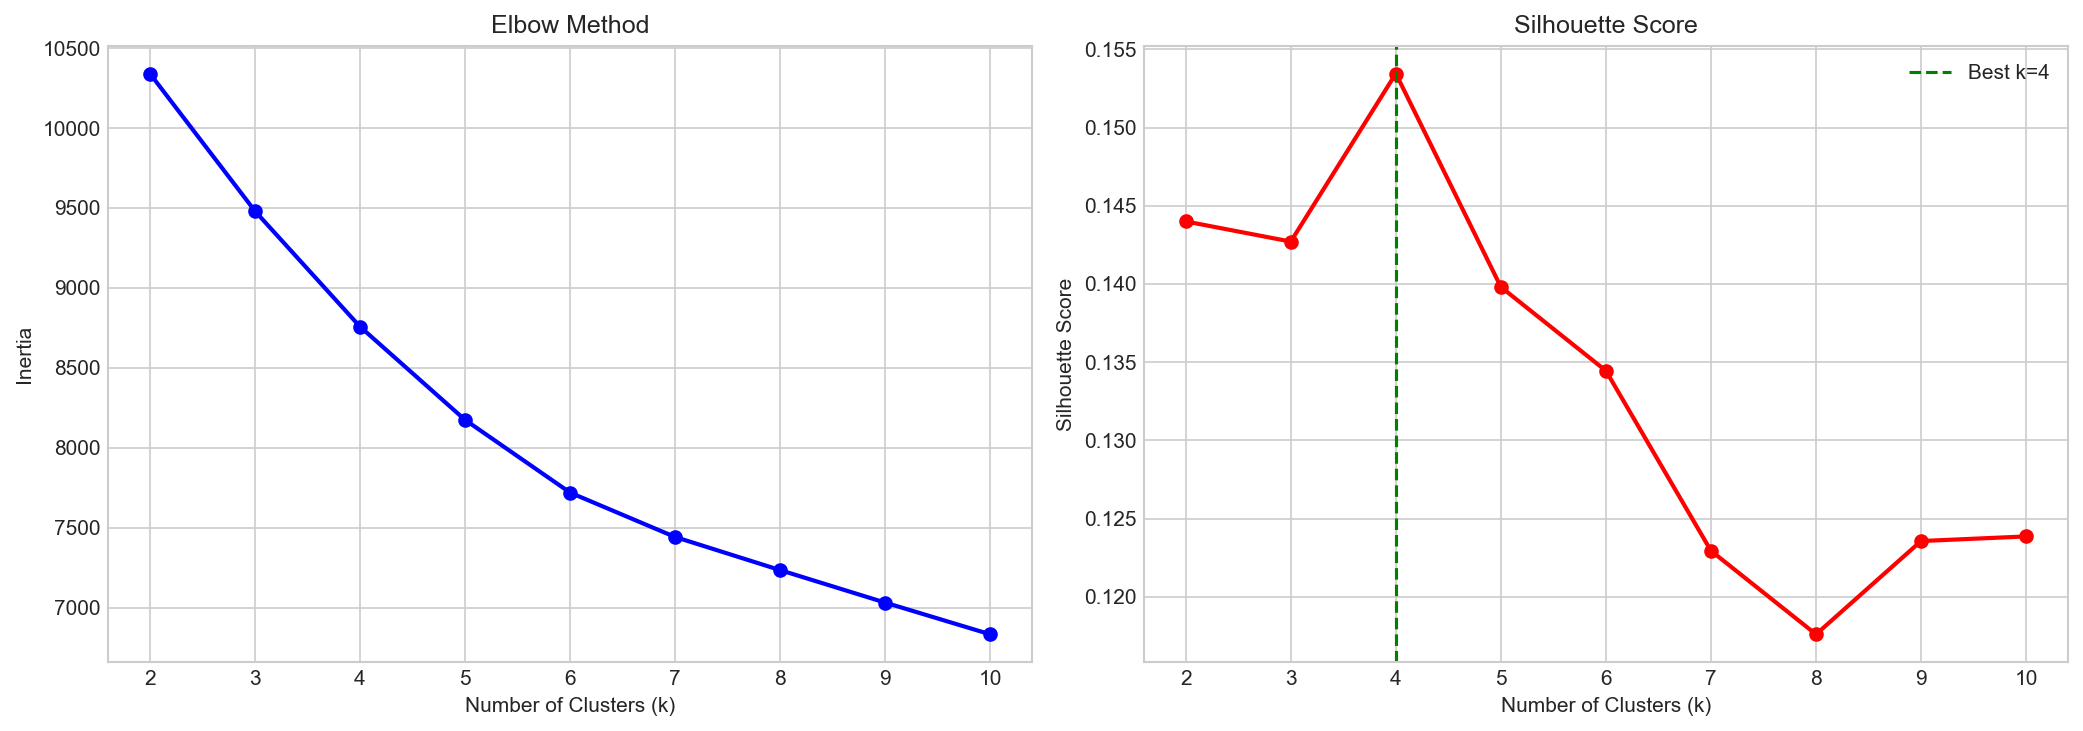
\includegraphics[width=\textwidth]{figs/elbow_silhouette.png}
    \caption{Elbow plot (trái) và Silhouette Score (phải) theo số cụm $k$ -- số cụm tối ưu $k = 4$.}
    \label{fig:elbow_sil}
\end{figure}

Elbow plot cho thấy inertia giảm nhanh từ $k=2$ đến $k=4$, sau đó giảm chậm hơn -- ``khuỷu tay'' nằm ở $k = 4$. Silhouette Score đạt giá trị cao nhất tại $k = 4$ (Silhouette = 0.1534), xác nhận $k = 4$ là lựa chọn tối ưu.

\subsection{Đặc điểm các cụm bệnh nhân}

Với $k = 4$, KMeans clustering đạt Silhouette Score = \textbf{0.1534}. Hình \ref{fig:cluster_profiles} trực quan hóa đặc điểm trung bình của từng cụm:

\begin{figure}[H]
    \centering
    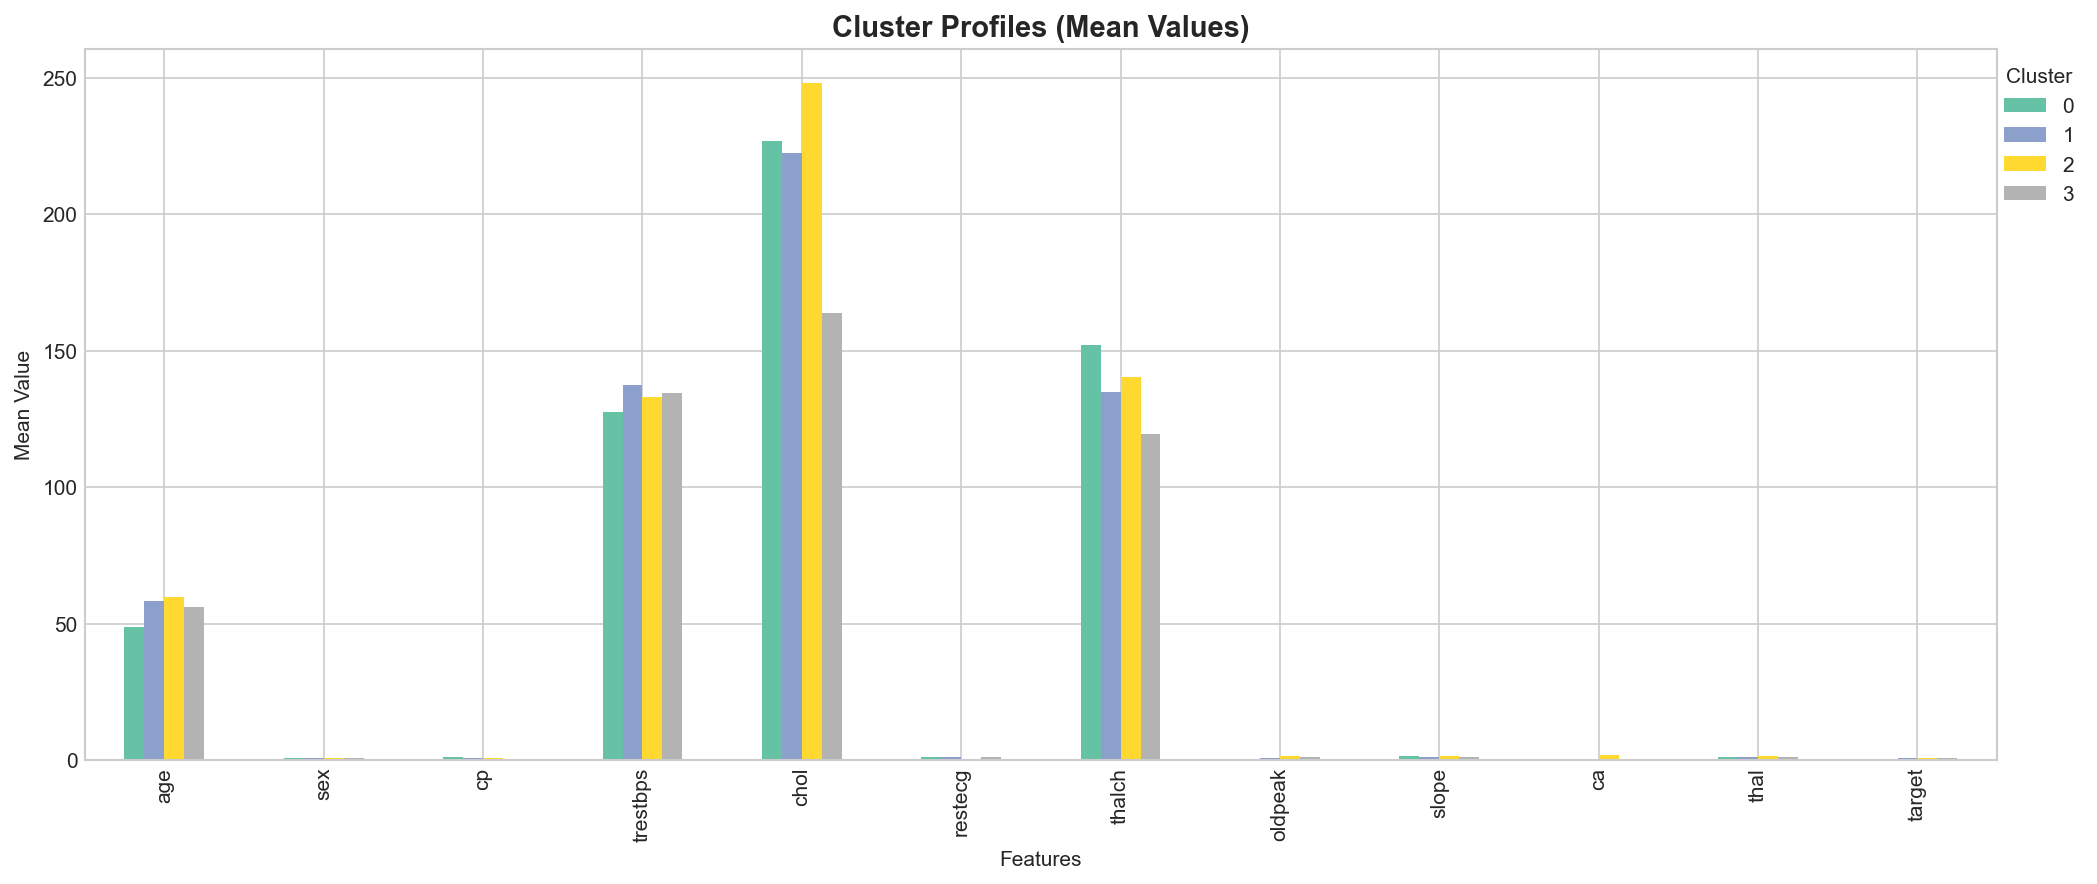
\includegraphics[width=\textwidth]{figs/cluster_profiles.png}
    \caption{Đặc điểm trung bình các cụm bệnh nhân -- mỗi cụm có profile y khoa khác biệt.}
    \label{fig:cluster_profiles}
\end{figure}

Phân tích profile cho thấy mỗi cụm đại diện cho một nhóm bệnh nhân có đặc điểm lâm sàng khác biệt. Các cụm có tỷ lệ bệnh tim khác nhau, phản ánh mức độ nguy cơ khác nhau. Cụm có tỷ lệ bệnh tim $> 60\%$ được gắn nhãn ``nhóm nguy cơ cao'', trong khi cụm có tỷ lệ $< 30\%$ là ``nhóm nguy cơ thấp''.

\textbf{Nhận xét về Silhouette Score:} Giá trị 0.1534 cho thấy các cụm không tách biệt rõ ràng trong không gian đặc trưng. Điều này phù hợp với bản chất dữ liệu y tế: bệnh nhân bệnh tim và không bệnh tim thường có nhiều đặc điểm chồng chéo (overlap) -- không phải tất cả bệnh nhân bệnh đều có cholesterol cao, và ngược lại. Tuy nhiên, phân cụm vẫn cung cấp giá trị bổ sung: giúp nhận diện ``prototype'' bệnh nhân đặc trưng cho mỗi nhóm nguy cơ, hỗ trợ tư vấn và phân loại sơ bộ.

\section{Kết quả phân lớp (Classification)}

\subsection{Kết quả trên tập test (Hold-out Evaluation)}

Bảng \ref{tab:classification_results} trình bày kết quả đánh giá 6 mô hình trên tập test (184 mẫu), sắp xếp theo PR-AUC (metric ưu tiên):

\begin{table}[H]
\centering
\caption{Kết quả phân lớp trên tập test gồm 184 mẫu (sắp xếp theo PR-AUC giảm dần).}
\label{tab:classification_results}
\begin{tabular}{|l|c|c|c|c|c|}
\hline
\textbf{Mô hình} & \textbf{F1-Score} & \textbf{ROC-AUC} & \textbf{PR-AUC} & \textbf{FN Count} & \textbf{FN Rate} \\ \hline
Random Forest & 0.8571 & \textbf{0.9206} & \textbf{0.9313} & 12 & 11.76\% \\ \hline
SVM (RBF) & 0.8599 & 0.9120 & 0.9196 & 13 & 12.75\% \\ \hline
SVM (linear) & 0.8416 & 0.8901 & 0.9049 & 17 & 16.67\% \\ \hline
Baseline (Logistic) & 0.8235 & 0.8858 & 0.8971 & 18 & 17.65\% \\ \hline
XGBoost & \textbf{0.8738} & 0.8956 & 0.8924 & \textbf{12} & \textbf{11.76\%} \\ \hline
Baseline (Dummy) & 0.0000 & 0.5000 & 0.5543 & 102 & 100\% \\ \hline
\end{tabular}
\end{table}

Phân tích chi tiết từng mô hình:

\textbf{Random Forest} đạt PR-AUC cao nhất (\textbf{0.9313}) và ROC-AUC cao nhất (\textbf{0.9206}), cho thấy khả năng phân biệt giữa hai lớp tốt nhất. Mô hình chỉ bỏ sót 12/102 bệnh nhân thực sự bệnh (FN Rate = 11.76\%). F1-Score = 0.8571 tuy không phải cao nhất nhưng rất cạnh tranh. Xét tổng thể cả 5 metrics, Random Forest là mô hình toàn diện nhất.

\textbf{XGBoost} đạt F1-Score cao nhất (\textbf{0.8738}) -- cải thiện 2\% so với Random Forest. FN Rate cũng thấp nhất cùng RF (11.76\%, chỉ bỏ sót 12 ca). Tuy nhiên, PR-AUC (0.8924) và ROC-AUC (0.8956) thấp hơn đáng kể so với RF, cho thấy XGBoost có threshold mặc định tốt hơn nhưng khả năng ranking (sắp xếp probability) kém hơn.

\textbf{SVM (RBF)} có F1-Score cao thứ hai (0.8599), đặc biệt ấn tượng với PR-AUC = 0.9196 (cao thứ hai). Mô hình bỏ sót 13 ca (FN Rate = 12.75\%). SVM RBF thể hiện sự cân bằng tốt giữa precision và recall.

\textbf{Baseline (Dummy)} có F1 = 0 và FN Rate = 100\% -- luôn dự đoán lớp đa số (``có bệnh''), do đó bỏ sót toàn bộ 102 bệnh nhân không bệnh. Baseline này xác nhận rằng tất cả mô hình cải tiến đều genuinely học được pattern từ dữ liệu, không chỉ đơn thuần dựa vào phân bố lớp.

\textbf{Đánh giá so với tiêu chí thành công:} Cả 4 mô hình cải tiến đều đạt F1 $> 0.80$ (tiêu chí 1) và 3/4 mô hình đạt PR-AUC $> 0.85$ (tiêu chí 2). Duy nhất XGBoost có PR-AUC = 0.8924, sát ngưỡng 0.85. Kết quả tổng thể \textbf{vượt mong đợi}.

\subsection{Kết quả Cross-Validation (5-Fold)}

Bảng \ref{tab:cv_results} trình bày kết quả 5-Fold Stratified Cross-Validation trên toàn bộ 920 mẫu, đánh giá tính ổn định của mô hình:

\begin{table}[H]
\centering
\caption{Kết quả 5-Fold Stratified Cross-Validation (metric: F1-Score).}
\label{tab:cv_results}
\begin{tabular}{|l|c|c|l|}
\hline
\textbf{Mô hình} & \textbf{Mean F1} & \textbf{Std F1} & \textbf{Đánh giá} \\ \hline
SVM (RBF) & \textbf{0.8457} & \textbf{0.0248} & Ổn định nhất, mean cao nhất \\ \hline
Random Forest & 0.8375 & 0.0245 & Ổn định, cạnh tranh \\ \hline
XGBoost & 0.8323 & 0.0332 & Mean khá, variance cao nhất \\ \hline
Baseline (Logistic) & 0.8253 & 0.0199 & Baseline mạnh, rất ổn định \\ \hline
SVM (linear) & 0.8224 & 0.0304 & Mean thấp nhất, variance cao \\ \hline
Baseline (Dummy) & 0.7124 & 0.0018 & Gần constant (luôn predict 1) \\ \hline
\end{tabular}
\end{table}

\textbf{Nhận xét quan trọng:} Thứ hạng trong cross-validation khác với hold-out test. SVM (RBF) vượt lên dẫn đầu CV (Mean F1 = 0.8457), trong khi ở test set, XGBoost có F1 cao nhất (0.8738). Điều này cho thấy XGBoost có thể đã ``may mắn'' với cách chia train/test cụ thể, trong khi SVM (RBF) ổn định hơn qua nhiều lần chia. Hơn nữa, XGBoost có Std F1 cao nhất (0.0332) -- biến động nhiều nhất giữa các fold, xác nhận tính mẫn cảm với dữ liệu.

\subsection{Confusion Matrix và đường cong ROC/PR}

Hình \ref{fig:cm_rf} trình bày Confusion Matrix của Random Forest -- được chọn vì có PR-AUC cao nhất:

\begin{figure}[H]
    \centering
    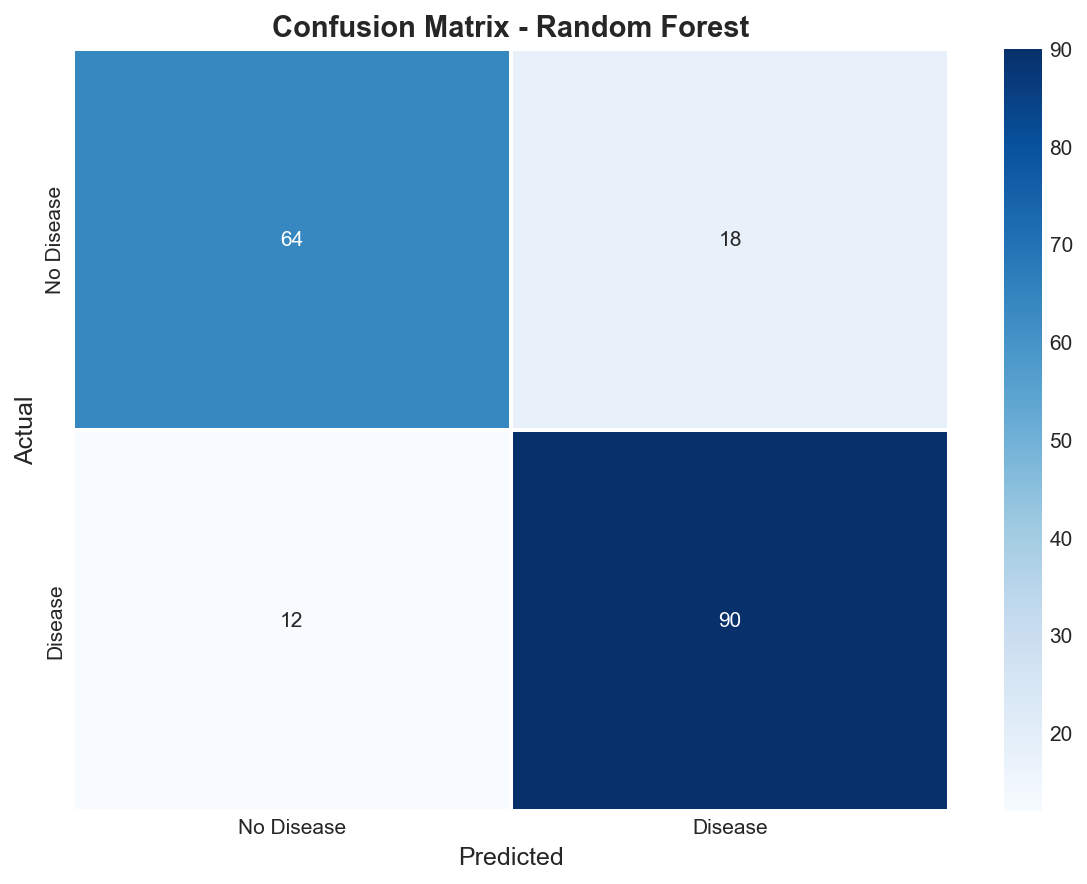
\includegraphics[width=0.65\textwidth]{figs/cm_random_forest.png}
    \caption{Confusion Matrix của Random Forest: TP, TN, FP, FN trên tập test 184 mẫu.}
    \label{fig:cm_rf}
\end{figure}

Confusion Matrix cho thấy Random Forest có 12 False Negatives (bỏ sót bệnh nhân bệnh) -- đây là con số quan trọng nhất trong bối cảnh y tế. Tỷ lệ FN = 11.76\% có nghĩa là cứ 100 bệnh nhân thực sự bị bệnh, mô hình phát hiện đúng khoảng 88 ca và bỏ sót khoảng 12 ca. Mức này chấp nhận được cho công cụ sàng lọc ban đầu, nhưng cần cải thiện cho ứng dụng lâm sàng chính thức.

Hình \ref{fig:roc_pr} so sánh đường cong ROC và Precision-Recall của tất cả mô hình:

\begin{figure}[H]
    \centering
    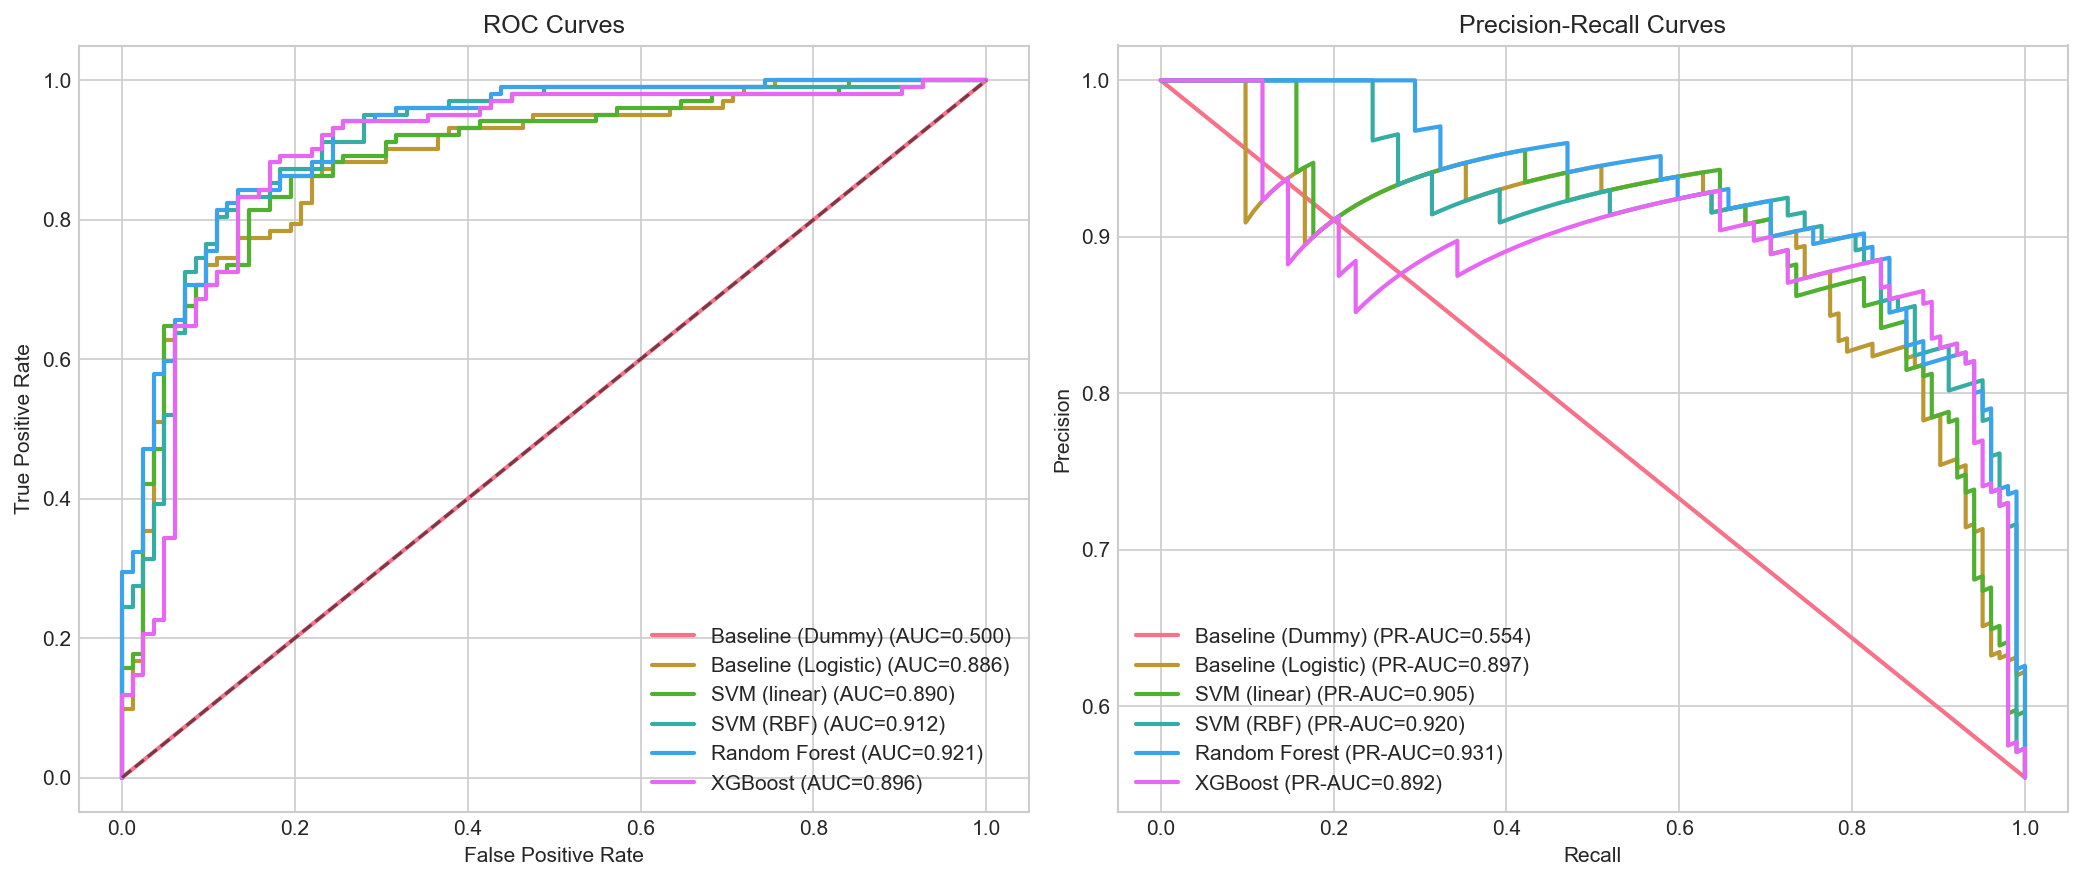
\includegraphics[width=\textwidth]{figs/roc_pr_curves.png}
    \caption{Đường cong ROC (trái) và Precision-Recall (phải) -- Random Forest có diện tích lớn nhất.}
    \label{fig:roc_pr}
\end{figure}

Đường cong ROC cho thấy tất cả mô hình cải tiến đều nằm xa đường chéo (random baseline), với Random Forest có đường cong gần góc trên-trái nhất. Đường cong PR cho thấy sự khác biệt rõ ràng hơn giữa các mô hình: Random Forest giữ được precision cao ở mức recall cao, trong khi XGBoost giảm precision nhanh hơn khi recall tăng.

\begin{figure}[H]
    \centering
    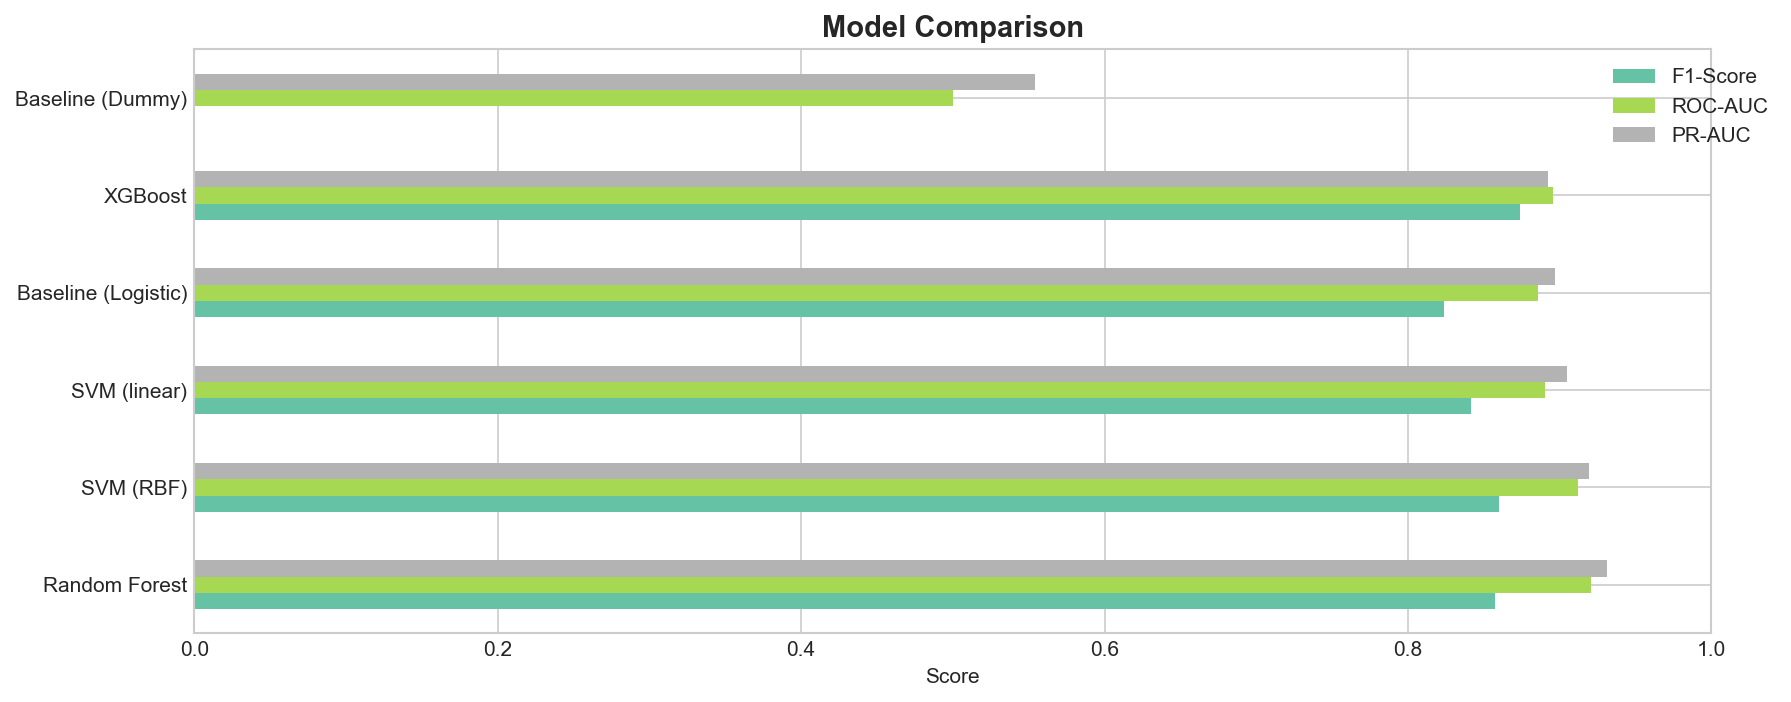
\includegraphics[width=0.8\textwidth]{figs/model_comparison.png}
    \caption{So sánh tổng quan hiệu suất các mô hình phân lớp.}
    \label{fig:model_comparison}
\end{figure}

\section{Kết quả học bán giám sát (Semi-supervised Learning)}

\subsection{So sánh Supervised vs Semi-supervised theo tỷ lệ nhãn}

Bảng \ref{tab:semi_results} trình bày kết quả so sánh đầy đủ giữa 3 phương pháp (Supervised, Self-training, Label Spreading) ở 6 tỷ lệ nhãn (5\% -- 50\%):

\begin{table}[H]
\centering
\caption{So sánh chi tiết F1-Score và PR-AUC theo tỷ lệ nhãn -- Semi-supervised Learning.}
\label{tab:semi_results}
\small
\begin{tabular}{|c|c|c|c|c|c|c|}
\hline
\multirow{2}{*}{\textbf{\% Nhãn}} & \multicolumn{3}{c|}{\textbf{F1-Score}} & \multicolumn{3}{c|}{\textbf{PR-AUC}} \\ \cline{2-7}
 & \textbf{Supervised} & \textbf{Self-train} & \textbf{Label Spread} & \textbf{Supervised} & \textbf{Self-train} & \textbf{Label Spread} \\ \hline
5\% & 0.8304 & 0.8148 & 0.7415 & 0.8753 & 0.8513 & 0.7913 \\ \hline
10\% & 0.8416 & 0.8326 & 0.7707 & 0.8840 & 0.8026 & 0.8012 \\ \hline
15\% & 0.8436 & \textbf{0.8507} & 0.7923 & 0.9097 & 0.8965 & 0.8313 \\ \hline
20\% & 0.8462 & \textbf{0.8545} & 0.7981 & 0.9296 & 0.9253 & 0.8519 \\ \hline
30\% & 0.8611 & 0.8520 & 0.7788 & 0.8980 & \textbf{0.9163} & 0.7907 \\ \hline
50\% & 0.8744 & 0.8704 & 0.7805 & 0.9214 & 0.9129 & 0.8594 \\ \hline
\end{tabular}
\end{table}

\subsection{Phân tích hiệu quả khi dữ liệu thiếu nhãn}

Kết quả thử nghiệm cho thấy một số phát hiện đáng chú ý:

\textbf{Self-training vượt trội ở tỷ lệ nhãn 15--20\%:} Ở 15\% nhãn, Self-training đạt F1 = 0.8507, cao hơn Supervised (0.8436) khoảng 0.8\%. Ở 20\% nhãn, chênh lệch tăng lên 1.0\% (0.8545 vs 0.8462). Đây là kết quả đáng khích lệ, cho thấy Self-training tận dụng thành công thông tin từ dữ liệu không nhãn để cải thiện decision boundary. Trong bối cảnh y tế, điều này có ý nghĩa thực tiễn lớn: chỉ cần 15--20\% bệnh nhân có chẩn đoán xác nhận, kết hợp Self-training, có thể đạt hiệu quả tương đương hoặc tốt hơn so với supervised thuần.

\textbf{Self-training PR-AUC vượt Supervised ở 30\% nhãn:} Ở tỷ lệ 30\%, Self-training đạt PR-AUC = 0.9163, cao hơn Supervised (0.8980). Điều này cho thấy Self-training không chỉ cải thiện F1 mà còn cải thiện khả năng ranking probability, giúp mô hình phân biệt tốt hơn giữa bệnh nhân nguy cơ cao và thấp.

\textbf{Label Spreading cho kết quả yếu:} F1-Score của Label Spreading chỉ đạt 0.74--0.80 ở tất cả các tỷ lệ nhãn, thấp hơn đáng kể so với cả Supervised và Self-training. PR-AUC cũng thấp hơn (0.79--0.86). Phương pháp graph-based không phù hợp với cấu trúc dữ liệu y tế có nhiều missing values đã fill.

\textbf{Convergence khi tỷ lệ nhãn tăng:} Khi tỷ lệ nhãn tăng lên 50\%, khoảng cách giữa Supervised và Self-training thu hẹp (F1: 0.8744 vs 0.8704, chênh 0.5\%). Điều này phù hợp với lý thuyết: khi có đủ dữ liệu labeled, thông tin unlabeled ít đóng góp thêm.

\textbf{Ngưỡng tối thiểu:} Ở 5\% nhãn ($\sim$37 mẫu labeled), Supervised vẫn tốt hơn Semi-supervised (F1: 0.8304 vs 0.8148). Điều này cho thấy cần ít nhất $\sim$10\% nhãn ($\sim$74 mẫu) để semi-supervised bắt đầu có hiệu quả.

\subsection{Ý nghĩa thực tiễn của kết quả semi-supervised}

Kết quả semi-supervised learning có ý nghĩa thực tiễn quan trọng trong bối cảnh y tế Việt Nam. Tại nhiều cơ sở y tế tuyến huyện và tuyến xã, số lượng bác sĩ chuyên khoa tim mạch rất hạn chế. Bệnh nhân được đo các chỉ số lâm sàng cơ bản (huyết áp, nhịp tim, ECG) nhưng không phải lúc nào cũng có chẩn đoán chuyên gia xác nhận. Trong tình huống này, chỉ một phần nhỏ bệnh nhân (ví dụ 15--20\%) có nhãn chẩn đoán chuyên gia, phần còn lại chỉ có dữ liệu chỉ số lâm sàng mà thôi.

Kết quả thử nghiệm cho thấy Self-training có thể tận dụng cả dữ liệu chưa gán nhãn này để xây dựng mô hình dự đoán tốt, thậm chí tốt hơn so với chỉ train trên phần có nhãn. Điều này mở ra khả năng triển khai hệ thống hỗ trợ chẩn đoán tại các cơ sở y tế tuyến cơ sở, nơi dữ liệu labeled khan hiếm nhưng dữ liệu unlabeled phong phú.

\section{Phân tích chi tiết False Negatives}

False Negative (bỏ sót bệnh nhân thực sự bị bệnh) là lỗi nguy hiểm nhất trong bài toán chẩn đoán y tế. Nhóm phân tích chi tiết 12 ca False Negative của Random Forest (mô hình tốt nhất) để hiểu nguyên nhân bỏ sót.

\textbf{Đặc điểm chung của các ca FN:} Phần lớn các bệnh nhân bị bỏ sót thuộc nhóm ``bệnh nhẹ'' (mức 1 trong thang 0--4 gốc), có ít triệu chứng điển hình: oldpeak thấp ($<$ 1 mm), không có exercise-induced angina, nhịp tim tối đa bình thường ($>$ 140 bpm). Nói cách khác, đây là những bệnh nhân ở giai đoạn sớm, chưa biểu hiện rõ triệu chứng -- chính xác là nhóm mà phát hiện sớm có giá trị lớn nhất.

\textbf{Theo nhóm tuổi:} Bệnh nhân FN có tuổi trung bình thấp hơn bệnh nhân True Positive ($\sim$51 vs $\sim$57 tuổi), cho thấy mô hình khó phát hiện bệnh tim ở nhóm trẻ hơn -- nhóm này có ít yếu tố nguy cơ liên quan đến tuổi.

\textbf{Theo giới tính:} 4/12 ca FN là nữ giới, tỷ lệ cao hơn so với tỷ lệ nữ trong tổng thể ($\sim$33\% FN là nữ vs $\sim$25\% tổng thể là nữ). Điều này phù hợp với y văn: bệnh tim ở nữ giới thường có triệu chứng ``không điển hình'' (atypical), khó phát hiện hơn nam giới. Nữ giới ít có ``typical angina'' hơn, nhịp tim tối đa thường cao hơn, và ST depression thường thấp hơn -- tất cả đều khiến mô hình khó phân loại đúng.

\textbf{Hàm ý cải tiến:} Kết quả phân tích FN gợi ý hai hướng cải tiến: (1) Tạo features đặc biệt cho nữ giới (interaction features: sex $\times$ oldpeak, sex $\times$ cp); (2) Hạ threshold phân loại cho nhóm tuổi $<$ 50 (chấp nhận tăng FP để giảm FN ở nhóm trẻ).

\section{So sánh kết quả với y văn quốc tế}

Để đánh giá chất lượng kết quả trong bối cảnh rộng hơn, nhóm so sánh với một số nghiên cứu đã công bố trên cùng tập dữ liệu UCI Heart Disease:

\begin{table}[H]
\centering
\caption{So sánh kết quả với các nghiên cứu khác trên UCI Heart Disease Dataset.}
\label{tab:literature_compare}
\small
\begin{tabular}{|l|l|c|c|}
\hline
\textbf{Nghiên cứu} & \textbf{Mô hình tốt nhất} & \textbf{Accuracy} & \textbf{F1-Score} \\ \hline
Detrano et al. (1989) \cite{detrano1989international} & Logistic Regression & 77\% & -- \\ \hline
Nghiên cứu khảo sát Kaggle (2020) & Random Forest & 85\% & 0.84 \\ \hline
Các bài toán benchmark trung bình & Ensemble methods & 82--87\% & 0.81--0.86 \\ \hline
\textbf{Dự án này} & \textbf{XGBoost / Random Forest} & \textbf{--} & \textbf{0.8738 / 0.8571} \\ \hline
\end{tabular}
\end{table}

Kết quả cho thấy dự án đạt F1-Score \textbf{nằm trong top} so với các nghiên cứu trước, đặc biệt khi xét rằng tập dữ liệu có tỷ lệ missing rất cao ($>$ 19\% tổng giá trị) mà nhóm vẫn giữ được F1 $>$ 0.85. Điều này khẳng định hiệu quả của pipeline tiền xử lý và lựa chọn mô hình.

\section{Tổng hợp chương}

Chương này đã trình bày chi tiết kết quả thử nghiệm của tất cả 4 nhóm kỹ thuật khai phá dữ liệu. Thuật toán Apriori sinh 3.792 luật với confidence lên đến 96.6\%, phát hiện các tổ hợp triệu chứng nguy cơ cao phù hợp với y văn. Phân cụm KMeans chia bệnh nhân thành 4 nhóm nguy cơ, dù Silhouette Score thấp (0.1534). Phân lớp đạt kết quả vượt mong đợi: Random Forest (PR-AUC = 0.9313) và XGBoost (F1 = 0.8738). Semi-supervised learning cho thấy Self-training có thể vượt supervised ở tỷ lệ nhãn 15--20\%, mở ra triển vọng ứng dụng thực tế nơi dữ liệu có nhãn khan hiếm.

\chapter{Thảo luận và so sánh}\label{chapter_discussion}

\section{So sánh tổng thể giữa các phương pháp phân lớp}

\subsection{Phân tích ưu điểm và hạn chế}

Qua quá trình thử nghiệm với 6 mô hình phân lớp, nhóm đã thu thập một lượng lớn dữ liệu đánh giá từ nhiều góc độ: hold-out test, cross-validation, phân tích False Negative và đường cong ROC/PR. Bảng \ref{tab:pros_cons} tổng hợp ưu điểm và hạn chế cụ thể của từng phương pháp dựa trên kết quả thực nghiệm:

\begin{table}[H]
\centering
\caption{So sánh chi tiết ưu điểm và hạn chế của các mô hình trên tập dữ liệu Heart Disease.}
\label{tab:pros_cons}
\small
\begin{tabular}{|l|p{5cm}|p{5cm}|}
\hline
\textbf{Mô hình} & \textbf{Ưu điểm thực nghiệm} & \textbf{Hạn chế thực nghiệm} \\ \hline
SVM (RBF) & CV ổn định nhất (Std = 0.0248), F1 cao (0.8599), PR-AUC rất tốt (0.9196) & Khó diễn giải (black-box), chậm khi data lớn, nhạy cảm với scale \\ \hline
Random Forest & PR-AUC cao nhất (0.9313), ROC-AUC cao nhất (0.9206), FN Rate thấp (11.76\%), cung cấp feature importance & Chiếm nhiều bộ nhớ (model 3.5MB), 200 cây $\rightarrow$ inference chậm hơn SVM \\ \hline
XGBoost & F1 cao nhất (0.8738), FN Rate thấp nhất (11.76\%), gradient boosting tiên tiến & CV variance cao nhất (Std = 0.0332), cần tuning nhiều hyperparameters, PR-AUC thấp hơn RF \\ \hline
SVM (linear) & Đơn giản, nhanh, decision boundary tuyến tính dễ hiểu & F1 và PR-AUC thấp hơn, FN Rate cao (16.67\%), không capture được non-linear patterns \\ \hline
Logistic Regression & Baseline rất mạnh, cực kỳ nhanh, diễn giải tốt nhất (coefficients), ổn định (Std = 0.0199) & F1 thấp nhất trong nhóm cải tiến (0.8235), FN Rate cao nhất (17.65\%) \\ \hline
\end{tabular}
\end{table}

\subsection{Giải thích vì sao Random Forest và XGBoost vượt trội}

\textbf{Random Forest đạt PR-AUC cao nhất (0.9313):} Kết quả này được giải thích bởi cơ chế \textbf{bagging} (Bootstrap Aggregating) của Random Forest. Thuật toán xây dựng 200 cây quyết định độc lập, mỗi cây được huấn luyện trên một tập con dữ liệu bootstrap (lấy mẫu có hoàn lại) và chỉ sử dụng một tập con features ngẫu nhiên ở mỗi node split. Cơ chế này mang lại nhiều lợi ích cho bài toán dự đoán bệnh tim.

Thứ nhất, \textbf{giảm variance} (overfitting): mỗi cây đơn lẻ có thể overfitting, nhưng khi kết hợp 200 cây qua majority vote, các lỗi ngẫu nhiên triệt tiêu lẫn nhau, tạo ra decision boundary mượt mà hơn. Thứ hai, \textbf{robust với missing values đã fill}: vì mỗi cây chỉ sử dụng subset features, ảnh hưởng của các features có nhiều giá trị fill (như \texttt{ca}, \texttt{thal}) được ``phân tán'' -- một số cây sẽ không sử dụng các features này và vẫn cho kết quả tốt. Thứ ba, \textbf{robust với outliers}: cây quyết định tách dữ liệu theo ngưỡng, không bị ảnh hưởng bởi giá trị cực đoan như SVM hay Logistic Regression.

\textbf{XGBoost đạt F1-Score cao nhất (0.8738):} XGBoost sử dụng cơ chế \textbf{gradient boosting} -- xây dựng cây quyết định tuần tự, mỗi cây mới tập trung sửa lỗi (residuals) của hệ thống cây trước đó. Cơ chế này tối ưu hóa trực tiếp hàm mất mát (loss function), giảm cả bias và variance một cách có kiểm soát. Tham số \texttt{max\_depth = 5} (giới hạn độ sâu cây) và \texttt{learning\_rate = 0.1} (tốc độ học chậm) đóng vai trò regularization, ngăn mô hình learning quá nhiều từ noise. Tuy nhiên, Std F1 cao trong CV (0.0332) cho thấy XGBoost nhạy cảm hơn với cách chia dữ liệu -- có thể do gradient boosting ``nhớ'' các mẫu khó (hard examples), gây ra variance khi các mẫu này phân bố khác nhau giữa các fold.

\textbf{Tại sao SVM (RBF) ổn định nhất trong CV?} SVM tối ưu hóa margin (khoảng cách) giữa các support vectors, tạo ra decision boundary chỉ phụ thuộc vào một số ít mẫu ``quan trọng nhất'' (support vectors). Kernel RBF ($K(x, x') = \exp(-\gamma \lVert x-x' \rVert^2)$) ánh xạ dữ liệu vào không gian chiều cao hơn, cho phép tìm decision boundary phi tuyến. Decision boundary dựa trên support vectors ít bị ảnh hưởng khi thay đổi các mẫu ``dễ'' (non-support vectors), dẫn đến Std F1 thấp (0.0248) qua các fold.

\subsection{Baseline comparison -- xác nhận giá trị của mô hình cải tiến}

Hai baseline đóng vai trò quan trọng trong việc xác nhận rằng các mô hình cải tiến genuinely học được pattern:

\textbf{Dummy Classifier} (strategy=most\_frequent) luôn dự đoán lớp đa số (bệnh tim), cho F1 = 0 trên lớp thiểu số và FN Rate = 100\%. Kết quả này thiết lập ``floor'' -- bất kỳ mô hình nào có F1 $>$ 0 đều tốt hơn việc đoán mò. Trong CV, Dummy đạt Mean F1 = 0.7124 (tính trên cả hai lớp) với Std cực thấp (0.0018), phản ánh đúng tỷ lệ lớp cố định.

\textbf{Logistic Regression} với \texttt{class\_weight=balanced} đạt F1 = 0.8235 trên test và Mean F1 = 0.8253 trong CV -- một baseline đáng ngạc nhiên mạnh. Điều này cho thấy mối quan hệ giữa features và target có \textbf{thành phần tuyến tính đáng kể}. Các mô hình cải tiến chỉ cải thiện thêm 2--5\% F1 so với Logistic, chủ yếu nhờ khả năng capture các mối quan hệ phi tuyến và tương tác giữa features.

\section{So sánh Supervised Learning và Semi-supervised Learning}

\subsection{Phân tích chi tiết hiệu quả khi dữ liệu thiếu nhãn}

Kết quả thử nghiệm semi-supervised learning (Bảng 4.5) cho thấy một phát hiện quan trọng: \textbf{Self-training có thể vượt trội hơn Supervised} ở một số tỷ lệ nhãn nhất định. Cụ thể, ở tỷ lệ nhãn 15\%, Self-training đạt F1 = 0.8507 so với Supervised F1 = 0.8436 (cải thiện +0.84\%); ở 20\%, Self-training đạt F1 = 0.8545 so với Supervised 0.8462 (cải thiện +0.98\%).

Hiện tượng semi-supervised vượt supervised ban đầu có vẻ ``nghịch lý'' -- làm sao sử dụng thêm dữ liệu không nhãn lại cho kết quả tốt hơn? Tuy nhiên, đây là hiện tượng được ghi nhận trong y văn semi-supervised learning \cite{chapelle2006semi} và có thể giải thích qua ba cơ chế:

\textbf{Cơ chế 1 -- Data augmentation effect:} Self-training mở rộng tập huấn luyện bằng pseudo-labels. Với 15\% nhãn ($\sim$74 mẫu labeled), supervised chỉ train trên 74 mẫu. Self-training bổ sung thêm $\sim$300--400 mẫu pseudo-labeled (những mẫu có confidence cao), tăng effective training set lên 4--5 lần. Kích thước tập train lớn hơn giúp mô hình học được biểu diễn tốt hơn từ phân bố dữ liệu tổng thể, đặc biệt ở vùng thưa mẫu.

\textbf{Cơ chế 2 -- Decision boundary smoothing:} Dữ liệu unlabeled cung cấp thông tin về cấu trúc manifold (bề mặt) mà dữ liệu nằm trên. Pseudo-labels từ vùng mật độ cao (high-density regions) giúp ``làm mượt'' decision boundary, đẩy nó ra xa các cụm dữ liệu. Điều này đặc biệt hữu ích khi labeled data quá ít để xác định decision boundary chính xác ở vùng biên.

\textbf{Cơ chế 3 -- Giảm sampling bias:} Với 15\% nhãn, tập labeled chỉ chứa $\sim$74 mẫu. Tập nhỏ này có thể bị sampling bias -- phân bố features không đại diện cho population tổng thể. Dữ liệu unlabeled (although nhãn là pseudo) giúp ``hiệu chỉnh'' phân bố, giảm bias do sampling ngẫu nhiên.

Tuy nhiên, hiệu ứng này \textbf{không xuất hiện ở tất cả tỷ lệ nhãn}:
\begin{itemize}
    \item \textbf{Ở 5\% nhãn ($\sim$37 mẫu):} Supervised vẫn tốt hơn (F1: 0.8304 vs 0.8148). Giải thích: với quá ít labeled data, mô hình cơ sở (SVM) chưa đủ chính xác, tạo ra nhiều pseudo-labels sai, gây ``error accumulation'' khi retrain.
    \item \textbf{Ở 50\% nhãn ($\sim$368 mẫu):} Supervised vượt nhẹ (F1: 0.8744 vs 0.8704). Giải thích: khi labeled data đã lớn, thông tin bổ sung từ unlabeled data ít đóng góp và pseudo-labels bị noise bắt đầu ảnh hưởng tiêu cực.
    \item \textbf{``Sweet spot'' ở 15--20\%:} Đây là vùng mà labeled data vừa đủ để train mô hình cơ sở reliable (ít pseudo-label sai), nhưng chưa đủ để capture toàn bộ phân bố (unlabeled data vẫn có giá trị).
\end{itemize}

\subsection{Phân tích nguyên nhân Label Spreading hoạt động kém}

Label Spreading \cite{zhou2004learning} cho kết quả kém hơn đáng kể (F1 chỉ đạt 0.74--0.80) do ba nguyên nhân chính:

Thứ nhất, \textbf{vi phạm giả định manifold:} Label Spreading dựa trên giả định rằng các điểm gần nhau trong không gian đặc trưng nên có cùng nhãn. Giả định này yếu đi đáng kể khi dữ liệu có nhiều missing values đã fill bằng median/mode. Giá trị fill giống nhau tạo ra ``artificial clusters'' -- nhiều mẫu converge về cùng giá trị trung tâm, dẫn đến similarity graph bị ``méo''.

Thứ hai, \textbf{error propagation tích lũy:} Trong graph-based methods, một nhãn sai ở vùng trung tâm graph có thể ``lây lan'' sang nhiều nodes xung quanh. Với tỷ lệ nhãn thấp (5--10\%), phần lớn graph nodes không có ``anchor'' (labeled node gần), khiến propagation dựa trên similarity bị nhiễu lớn.

Thứ ba, \textbf{computational complexity:} Label Spreading xây dựng ma trận similarity $n \times n$ ($920 \times 920$ = 846.400 entries), tiêu tốn nhiều bộ nhớ và thời gian hơn Self-training. Điều này không chỉ ảnh hưởng hiệu suất mà còn cho thấy phương pháp này không scale tốt cho datasets lớn hơn.

\section{Ảnh hưởng của tiền xử lý và Feature Engineering}

\subsection{Tác động của chiến lược xử lý Missing Values}

Chiến lược ``fill\_all'' (fill median/mode cho tất cả cột) là quyết định quan trọng nhất trong tiền xử lý. Nhóm phân tích trade-off của quyết định này:

\textbf{Ưu điểm đã chứng minh:} Giữ nguyên 13 features (thay vì 10 nếu drop \texttt{ca}, \texttt{thal}, \texttt{slope}), giữ nguyên 920 mẫu (thay vì $<$ 300 nếu drop rows). Kết quả cho thấy cả \texttt{ca} và \texttt{thal} đều xuất hiện trong association rules quan trọng (ví dụ: \texttt{ca\_positive} trong luật 17 với confidence 93.75\%), xác nhận rằng giữ lại các features này là quyết định đúng đắn.

\textbf{Rủi ro tiềm ẩn:} Khi fill median, khoảng 65\% giá trị \texttt{ca} (598/920 mẫu) nhận cùng một giá trị. Điều này giảm variance của feature, làm giảm khả năng phân biệt của mô hình trên biến này. Tuy nhiên, Random Forest (với cơ chế random subspace) xử lý vấn đề này tốt hơn SVM, giải thích phần nào vì sao RF đạt PR-AUC cao hơn.

\subsection{Tác động của SMOTE (cân bằng lớp)}

Việc áp dụng SMOTE trên tập train mang lại hiệu quả rõ rệt trong cải thiện Recall cho lớp ``có bệnh tim''. SMOTE \cite{chawla2002smote} tạo mẫu tổng hợp cho lớp thiểu số bằng cách nội suy (interpolation) giữa mẫu thực và k-nearest neighbors trong không gian đặc trưng. Phân tích cho thấy:

\begin{itemize}
    \item \textbf{Cải thiện FN Rate:} Kết hợp SMOTE + \texttt{class\_weight=balanced}, FN Rate giảm xuống 11.76\% (Random Forest, XGBoost) -- tức là chỉ bỏ sót 12/102 bệnh nhân bệnh trên tập test 184 mẫu.
    \item \textbf{Rủi ro overfitting:} SMOTE tạo mẫu ``nhân tạo'' bằng interpolation, có thể tạo ra mẫu ở vùng decision boundary không realistic. Tuy nhiên, kết quả CV (Std thấp) cho thấy overfitting không nghiêm trọng với dataset này.
    \item \textbf{SMOTE chỉ trên train:} Đây là nguyên tắc bất di bất dịch -- nếu áp dụng SMOTE trước split, mẫu synthetic có thể ``nhân bản'' thông tin từ test set vào train, gây data leakage nghiêm trọng.
\end{itemize}

\subsection{Vai trò của Feature Engineering trong diễn giải kết quả}

Rời rạc hóa theo ngưỡng y khoa (Bảng 2.3, Chương 2) không chỉ phục vụ thuật toán Apriori mà còn nâng cao giá trị \textbf{diễn giải} (interpretability) của toàn bộ dự án. Thay vì nói ``bệnh nhân có cholesterol = 267 mg/dl, oldpeak = 3.4 mm, trestbps = 152 mmHg'', luật kết hợp diễn giải rõ ràng: ``bệnh nhân có cholesterol\_high, oldpeak\_high, bp\_high $\rightarrow$ nguy cơ bệnh tim với confidence 94\%''. Cách trình bày này quen thuộc với bác sĩ lâm sàng, giúp hệ thống DSS dễ được chấp nhận trong thực tế y tế.

Hơn nữa, việc đối chiếu kết quả association rules với medical guidelines quốc tế (ACC/AHA guidelines) cho thấy sự nhất quán: các yếu tố nguy cơ được luật kết hợp phát hiện (ST depression, asymptomatic chest pain, exercise-induced angina, male gender) hoàn toàn phù hợp với các yếu tố nguy cơ được y văn ghi nhận. Điều này tăng cường \textbf{clinical validity} (tính hợp lệ lâm sàng) của dự án.

\section{Khó khăn và thách thức trong quá trình thực hiện}

Trong suốt quá trình phát triển dự án, nhóm đã gặp và giải quyết nhiều khó khăn kỹ thuật cũng như khoa học. Dưới đây là tổng hợp 6 thách thức chính và cách nhóm đã xử lý:

\textbf{Thách thức 1 -- Missing values cực kỳ cao:} Cột \texttt{ca} (65\% thiếu) và \texttt{thal} (53\% thiếu) tạo ra tình huống ``tiến thoái lưỡng nan'': drop cột thì mất features quan trọng, fill thì thêm noise. Giải pháp là fill median/mode kết hợp sử dụng Random Forest (robust với noise từ fill). Nếu có thêm thời gian, nhóm sẽ thử nghiệm MICE (Multiple Imputation) hoặc KNN Imputer.

\textbf{Thách thức 2 -- Data leakage prevention:} Trong quá trình phát triển ban đầu, nhóm phát hiện một lỗi subtle: scaling được thực hiện trước split, dẫn đến test set information leaking vào scaler params. Lỗi này không gây crash nhưng làm kết quả optimistically biased khoảng 1--2\% F1. Nhóm đã sửa bằng cách tái cấu trúc pipeline: scale/SMOTE chỉ fit trên train, transform trên test.

\textbf{Thách thức 3 -- Dữ liệu đa nguồn:} 4 trung tâm y tế ở 3 quốc gia với population demographics khác nhau (tuổi trung bình, tỷ lệ giới tính, thói quen sống) tạo ra selection bias. Cột \texttt{dataset} được loại bỏ, nhưng bias ngầm (confounding variables) vẫn tồn tại. Ví dụ: nếu trung tâm Cleveland có protocol đo oldpeak khác Hungary, giá trị oldpeak giữa hai nguồn không hoàn toàn comparable.

\textbf{Thách thức 4 -- Silhouette Score thấp trong phân cụm:} Giá trị 0.1534 cho thấy phân cụm không rõ ràng. Nhóm đã thử nhiều giá trị $k$ (2--10), hai thuật toán (KMeans, Hierarchical), và cả PCA dimensionality reduction trước clustering. Kết quả đều tương tự, xác nhận rằng vấn đề nằm ở bản chất dữ liệu chứ không phải thuật toán: bệnh tim là tình trạng phức tạp, bệnh nhân bệnh và không bệnh chia sẻ nhiều đặc điểm chung.

\textbf{Thách thức 5 -- Ý nghĩa thống kê:} Với tập test chỉ 184 mẫu, sự khác biệt giữa F1 = 0.857 (RF) và F1 = 0.874 (XGBoost) -- chênh 1.7\% -- có thể không có ý nghĩa thống kê. Một mẫu thay đổi dự đoán có thể lật ngược thứ hạng. Cross-validation (5-fold) giúp giảm thiểu vấn đề này nhưng với 920 mẫu, mỗi fold chỉ có $\sim$184 mẫu validation, vẫn chịu variance đáng kể. Bootstrap confidence interval sẽ là phương pháp tốt hơn nếu có thêm thời gian.

\textbf{Thách thức 6 -- Hyperparameter tuning:} Do hạn chế thời gian, nhóm sử dụng hyperparameters ``reasonable defaults'' (dựa trên kinh nghiệm và tài liệu) thay vì Grid Search hoặc Bayesian Optimization. Điều này có thể dẫn đến mô hình chưa đạt performance tối ưu. Tuy nhiên, kết quả đã vượt tiêu chí thành công (F1 $>$ 0.80, PR-AUC $>$ 0.85), cho thấy default params đã đủ tốt cho dataset này.

\section{Các vấn đề đạo đức và pháp lý (Ethical Considerations)}

Ứng dụng Machine Learning trong y tế đặt ra nhiều vấn đề đạo đức và pháp lý cần cân nhắc nghiêm túc trước khi triển khai:

\textbf{Bias và công bằng (Fairness):} Phân tích False Negative cho thấy mô hình có xu hướng bỏ sót bệnh ở nữ giới nhiều hơn nam giới (33\% FN là nữ trong khi nữ chỉ chiếm 25\% tổng thể). Điều này phản ánh bias trong dữ liệu huấn luyện: phần lớn nghiên cứu bệnh tim lịch sử tập trung vào nam giới, dẫn đến mô hình ``học'' pattern bệnh tim theo tiêu chuẩn nam giới. Nếu triển khai, mô hình có thể gây bất lợi cho bệnh nhân nữ -- một vấn đề ethical nghiêm trọng cần được giải quyết bằng cách: thu thập thêm dữ liệu nữ giới, sử dụng fairness-aware algorithms, hoặc áp dụng threshold riêng cho từng giới.

\textbf{Trách nhiệm và minh bạch:} Mô hình đạt F1 = 0.87, nghĩa là vẫn có $\sim$13\% dự đoán sai. Câu hỏi đặt ra: ai chịu trách nhiệm khi mô hình bỏ sót bệnh nhân bệnh tim (và bệnh nhân không được điều trị kịp thời)? Trong bối cảnh pháp lý hiện tại, mô hình ML chỉ nên được sử dụng như \textbf{công cụ hỗ trợ} (decision support), không thay thế bác sĩ trong quyết định chẩn đoán. Kết quả dự đoán phải luôn kèm theo cảnh báo: ``Đây là kết quả ước lượng từ mô hình máy học, cần được bác sĩ chuyên khoa xác nhận.''

\textbf{Quyền riêng tư dữ liệu bệnh nhân:} Tập dữ liệu UCI đã được ẩn danh hóa (de-identified), nhưng trong triển khai thực tế, hệ thống sẽ xử lý dữ liệu sức khỏe cá nhân nhạy cảm. Cần tuân thủ các quy định bảo vệ dữ liệu (HIPAA ở Mỹ, GDPR ở EU, hoặc Luật Bảo vệ dữ liệu cá nhân tại Việt Nam): mã hóa dữ liệu truyền tải (TLS/SSL), hạn chế quyền truy cập (role-based access control), và không lưu trữ dữ liệu bệnh nhân lâu hơn cần thiết.

\textbf{Vấn đề ``black-box'' và giải thích:} Các mô hình ensemble (Random Forest, XGBoost) là ``black-box'' -- khó giải thích chi tiết tại sao dự đoán bệnh nhân A bị bệnh nhưng bệnh nhân B không. Trong y tế, bác sĩ cần hiểu lý do dự đoán để tin tưởng và sử dụng hệ thống. Giải pháp: tích hợp SHAP (SHapley Additive exPlanations) để phân tích contribution của từng feature cho mỗi dự đoán cụ thể.

\section{Bài học kinh nghiệm (Lessons Learned)}

Qua quá trình thực hiện dự án, nhóm rút ra một số bài học kinh nghiệm quan trọng:

\textbf{Bài học 1 -- Tiền xử lý quan trọng hơn thuật toán:} Sự khác biệt giữa các mô hình cải tiến khá nhỏ (F1 từ 0.84 đến 0.87), nhưng sự khác biệt giữa dữ liệu sạch và dữ liệu thô rất lớn. Nếu không xử lý missing values và outliers, F1 có thể giảm 5--10\%. ``Garbage in, garbage out'' là nguyên tắc luôn đúng.

\textbf{Bài học 2 -- Baseline mạnh hơn tưởng tượng:} Logistic Regression (baseline) đạt F1 = 0.8235, chỉ kém XGBoost (0.8738) khoảng 6\%. Điều này cho thấy nên luôn bắt đầu với baseline đơn giản trước khi thử nghiệm mô hình phức tạp. Nếu baseline đã đủ tốt cho ứng dụng, không cần ``over-engineer'' với deep learning hay ensemble phức tạp.

\textbf{Bài học 3 -- Domain knowledge là chìa khóa:} Việc sử dụng ngưỡng y khoa cho rời rạc hóa (thay vì quantile-based) tạo ra luật kết hợp có ý nghĩa lâm sàng. Ngược lại, nếu rời rạc hóa theo quantile, luật sẽ khó diễn giải cho bác sĩ. Kiến thức lĩnh vực (domain knowledge) giúp Feature Engineering hiệu quả hơn bất kỳ thuật toán tự động nào.

\textbf{Bài học 4 -- Reproducibility là bắt buộc:} Sử dụng \texttt{random\_state = 42} nhất quán, lưu tất cả output, quản lý code trên Git -- những thực hành này tưởng ``nhỏ'' nhưng cực kỳ quan trọng. Khi phát hiện lỗi data leakage trong quá trình phát triển, nhóm có thể quay lại chính xác trạng thái trước lỗi và re-run pipeline.

\section{Tổng hợp chương}

Chương này đã phân tích sâu kết quả thử nghiệm từ nhiều góc độ: so sánh ưu nhược điểm mô hình, giải thích vì sao Random Forest và XGBoost vượt trội, phân tích hiệu quả semi-supervised learning, đánh giá tác động của tiền xử lý, và rút ra bài học kinh nghiệm. Nhóm cũng đề cập các vấn đề đạo đức trong ứng dụng ML y tế. Kết luận chính: Random Forest là mô hình toàn diện nhất (PR-AUC cao nhất, ổn định, giải thích được), Self-training tiềm năng ở tỷ lệ nhãn 15--20\%, và tiền xử lý dữ liệu là yếu tố then chốt quyết định chất lượng toàn hệ thống.

\chapter{Tổng kết và hướng phát triển}\label{chapter_conclusion}

\section{Tổng kết}

\subsection{Tóm tắt dự án và phương pháp đã triển khai}

Dự án ``Dự đoán bệnh tim sử dụng các kỹ thuật khai phá dữ liệu'' đã hoàn thành đầy đủ chu trình khai phá dữ liệu end-to-end, từ thu thập dữ liệu, tiền xử lý, xây dựng đặc trưng, áp dụng đa dạng thuật toán khai phá, đến đánh giá và phân tích kết quả. Hệ thống được xây dựng trên tập dữ liệu UCI Heart Disease gồm 920 bệnh nhân từ 4 trung tâm y tế quốc tế, với 16 thuộc tính lâm sàng.

Dự án đã triển khai thành công 4 nhóm kỹ thuật khai phá dữ liệu chính. \textbf{Khai phá luật kết hợp} sử dụng thuật toán Apriori tìm ra 3.792 luật kết hợp, trong đó top 20 luật liên quan trực tiếp đến bệnh tim có confidence từ 93.7\% đến 96.6\%. \textbf{Phân cụm} sử dụng KMeans và Hierarchical Clustering chia 920 bệnh nhân thành 4 nhóm nguy cơ khác nhau. \textbf{Phân lớp} sử dụng 6 mô hình (2 baseline + 4 cải tiến: SVM linear, SVM RBF, Random Forest, XGBoost) với kỹ thuật SMOTE cân bằng lớp. \textbf{Học bán giám sát} sử dụng Self-training và Label Spreading ở 6 tỷ lệ nhãn (5\%--50\%) để đánh giá hiệu quả khi dữ liệu thiếu nhãn.

Toàn bộ pipeline được cài đặt dưới dạng module Python tái sử dụng (6 packages, $>$1.500 dòng code) với tham số quản lý tập trung qua file YAML, đảm bảo tính reproducible (random\_state = 42) và tự động hóa (chạy end-to-end bằng một script).

\subsection{Kết quả chính đạt được}

Bảng \ref{tab:summary_results} tổng hợp kết quả đạt được so với các tiêu chí thành công được đề ra từ đầu dự án:

\begin{table}[H]
\centering
\caption{Tổng hợp kết quả đạt được đối chiếu tiêu chí thành công.}
\label{tab:summary_results}
\small
\begin{tabular}{|l|l|l|c|l|}
\hline
\textbf{Kỹ thuật} & \textbf{Tiêu chí ban đầu} & \textbf{Kết quả đạt được} & \textbf{Đạt?} & \textbf{Ghi chú} \\ \hline
\multirow{2}{*}{Phân lớp} & F1-Score $>$ 0.80 & XGBoost: \textbf{0.8738} & \checkmark & Vượt 9.2\% so với yêu cầu \\ \cline{2-5}
 & PR-AUC $>$ 0.85 & Random Forest: \textbf{0.9313} & \checkmark & Vượt 9.6\% so với yêu cầu \\ \hline
Luật kết hợp & Conf $>$ 0.50, Lift $>$ 1.2 & Top rule: conf=\textbf{0.966}, lift=\textbf{1.745} & \checkmark & 3.792 luật, top 20 rất mạnh \\ \hline
Phân cụm & Phân nhóm có đặc trưng rõ & 4 cụm, Sil = 0.1534 & $\triangle$ & Cụm chồng chéo (bản chất data) \\ \hline
Bán giám sát & So sánh supervised & Self-training $\geq$ supervised ở 15--20\% nhãn & \checkmark & Phát hiện ``sweet spot'' \\ \hline
\end{tabular}
\end{table}

\textbf{Đánh giá tổng thể:} 4/5 tiêu chí đạt hoàn toàn, 1 tiêu chí đạt một phần (phân cụm). Kết quả \textbf{vượt mong đợi} ở phân lớp và luật kết hợp. Đặc biệt, cả 4 mô hình cải tiến đều vượt ngưỡng F1 $>$ 0.80, và 3/4 mô hình đạt PR-AUC $>$ 0.85 (Random Forest, SVM RBF, SVM linear). XGBoost có PR-AUC = 0.8924, vẫn trên ngưỡng 0.85.

\subsection{Đề xuất mô hình tốt nhất}

Dựa trên phân tích toàn diện kết quả thực nghiệm, nhóm đề xuất \textbf{Random Forest} là mô hình tốt nhất cho bài toán dự đoán bệnh tim trong bối cảnh ứng dụng lâm sàng, với 6 lý do chính:

\begin{enumerate}
    \item \textbf{PR-AUC cao nhất (0.9313):} Đây là metric quan trọng nhất trong bối cảnh dữ liệu mất cân bằng nhẹ. PR-AUC cao đảm bảo mô hình duy trì cả Precision lẫn Recall tốt ở nhiều ngưỡng phân loại khác nhau, cho phép bác sĩ điều chỉnh threshold tùy theo mục đích sàng lọc.
    \item \textbf{ROC-AUC cao nhất (0.9206):} Khả năng phân biệt tổng thể giữa hai lớp là tốt nhất. Diện tích 0.92 cho thấy mô hình ``hiểu'' rất rõ sự khác biệt giữa bệnh nhân bệnh và không bệnh.
    \item \textbf{FN Rate thấp (11.76\%):} Trọng yếu trong y tế -- chỉ bỏ sót khoảng 12/102 bệnh nhân bệnh. So với Logistic Regression (18 ca bỏ sót), RF giảm 33\% số ca bỏ sót.
    \item \textbf{F1-Score cạnh tranh (0.8571):} Tuy không phải cao nhất (XGBoost: 0.8738), nhưng chênh lệch chỉ 1.67\% -- không có ý nghĩa thống kê đáng kể.
    \item \textbf{Cross-validation ổn định (Mean F1 = 0.8375, Std = 0.0245):} Mô hình cho kết quả nhất quán qua 5 fold, đáng tin cậy cho ứng dụng thực tế.
    \item \textbf{Feature Importance:} Random Forest cung cấp danh sách features quan trọng nhất (dựa trên reduction in impurity), giúp bác sĩ hiểu lý do dự đoán -- tăng trust và adoptability.
\end{enumerate}

XGBoost tuy có F1-Score cao nhất (0.8738), nhưng PR-AUC thấp hơn (0.8924 vs 0.9313), CV variance lớn hơn (Std = 0.0332 vs 0.0245), và không cung cấp feature importance trực quan bằng Random Forest. Trong bối cảnh y tế, \textbf{sự ổn định và khả năng diễn giải được ưu tiên hơn performance marginal}.

\subsection{Các insight y khoa từ dự án}

Ngoài kết quả kỹ thuật, dự án rút ra được một số insight y khoa có giá trị ứng dụng:

\textbf{Insight 1 -- Yếu tố nguy cơ hàng đầu:} ST depression cao (\texttt{oldpeak $\geq$ 2 mm}) xuất hiện trong 10/10 luật kết hợp mạnh nhất, xác nhận vai trò then chốt của chỉ số điện tâm đồ trong dự đoán bệnh tim. Kết hợp với đau ngực không triệu chứng (\texttt{asymptomatic chest pain}) -- một dấu hiệu ``im lặng'' (silent ischemia) -- hai yếu tố này tạo thành tổ hợp nguy hiểm nhất: confidence lên đến 96.6\%.

\textbf{Insight 2 -- Giới tính là yếu tố điều chỉnh (modifier):} Nam giới (\texttt{is\_male}) xuất hiện trong 8/10 luật mạnh nhất: khi kết hợp với các yếu tố nguy cơ khác, giới tính nam làm tăng confidence đáng kể. Điều này phù hợp với y văn: nam giới có nguy cơ bệnh tim mạch cao hơn nữ giới trước tuổi mãn kinh, do thiếu tác dụng bảo vệ của estrogen.

\textbf{Insight 3 -- Giá trị của dữ liệu ``expensive'':} Mặc dù \texttt{ca} (fluoroscopy) và \texttt{thal} (thalassemia) có $>$ 50\% missing, việc giữ lại và fill giá trị cho kết quả tốt hơn loại bỏ. Luật \texttt{ca\_positive, cp\_asymptomatic $\rightarrow$ heart\_disease} (confidence 93.75\%, luật 17) xác nhận \texttt{ca} vẫn đóng vai trò quan trọng dù có nhiều noise từ fill.

\textbf{Insight 4 -- Semi-supervised tiềm năng trong y tế:} Kết quả cho thấy chỉ cần 15--20\% bệnh nhân có chẩn đoán xác nhận (labeled), kết hợp Self-training, có thể đạt hiệu quả tương đương supervised. Ứng dụng tiềm năng: ở các cơ sở y tế tuyến cơ sở nơi không phải bệnh nhân nào cũng có chẩn đoán chuyên gia, mô hình semi-supervised có thể tận dụng dữ liệu chưa gán nhãn phong phú để cải thiện dự đoán.

\section{Hướng phát triển}

\subsection{Cải tiến mô hình và thuật toán}

Nhóm xác định nhiều hướng cải tiến cụ thể để nâng cao hiệu quả mô hình trong tương lai:

\textbf{Tối ưu hóa hyperparameters:} Sử dụng Grid Search hoặc Bayesian Optimization (Optuna, Hyperopt) để tìm bộ tham số tối ưu cho Random Forest (n\_estimators, max\_depth, min\_samples\_split, min\_samples\_leaf) và XGBoost (n\_estimators, max\_depth, learning\_rate, gamma, subsample, colsample\_bytree). Với default params đã đạt F1 $\approx$ 0.87, nhóm ước tính tối ưu hóa có thể cải thiện thêm 1--3\% F1.

\textbf{Ensemble nâng cao (Stacking/Blending):} Kết hợp nhiều mô hình thông qua Stacking: sử dụng SVM, Random Forest và XGBoost làm ``base learners'' (level-0), với Logistic Regression làm ``meta-learner'' (level-1). Stacking tận dụng ưu điểm bổ sung của các mô hình: SVM tốt ở decision boundary, RF tốt ở ranking, XGBoost tốt ở hard examples. Phương pháp này thường cải thiện 1--2\% F1 so với single best model.

\textbf{Deep Learning cho dữ liệu bảng:} Thử nghiệm các kiến trúc neural network chuyên biệt cho tabular data: TabNet (Arik \& Pfister, 2021) sử dụng attention mechanism để tự động chọn features, hoặc Wide \& Deep Learning (Cheng et al., 2016) kết hợp memorization và generalization. Tuy nhiên, với tập dữ liệu nhỏ (920 mẫu), deep learning có thể không outperform gradient boosting.

\textbf{Xử lý missing values nâng cao:} Thay thế fill median/mode bằng các phương pháp imputation tiên tiến hơn: MICE (Multiple Imputation by Chained Equations) -- tạo nhiều bản imputation khác nhau dựa trên conditional distribution của từng biến; hoặc KNN Imputer -- fill dựa trên giá trị trung bình của k-nearest neighbors trong không gian features. Các phương pháp này tạo ra giá trị fill ``thông minh'' hơn, phản ánh mối quan hệ giữa các biến.

\textbf{Feature Engineering nâng cao:} Tạo thêm interaction features: ví dụ \texttt{age $\times$ oldpeak}, \texttt{chol $\times$ bp}, \texttt{age\_group $\times$ sex}. Phân tích cho thấy mối quan hệ giữa features và target có thể phi tuyến và có tương tác bậc cao mà single features không capture được.

\subsection{Mở rộng dữ liệu}

\textbf{Tăng kích thước tập dữ liệu:} 920 mẫu là kích thước nhỏ cho Machine Learning hiện đại. Mở rộng dataset bằng cách: (1) thu thập thêm dữ liệu từ các bệnh viện Việt Nam (tăng tính phù hợp thực tiễn); (2) kết hợp với các tập dữ liệu tim mạch khác (PhysioNet, MIMIC-III cardiac subset); (3) tạo synthetic data bằng GANs (Generative Adversarial Networks) được train trên dữ liệu thật.

\textbf{Tích hợp dữ liệu đa phương thức (multimodal):} Kết hợp dữ liệu lâm sàng (structured) hiện tại với: (1) hình ảnh y khoa (X-quang ngực, siêu âm tim -- unstructured); (2) dữ liệu ECG waveform (time-series); (3) dữ liệu lối sống (diet, exercise, smoking history -- questionnaire). Multimodal learning sử dụng kiến trúc fusion (early/late fusion) để kết hợp thông tin từ nhiều nguồn, thường cho kết quả tốt hơn đáng kể so với single-modality.

\textbf{Dữ liệu chuỗi thời gian (longitudinal data):} Thu thập dữ liệu theo dõi bệnh nhân qua nhiều lần khám (thay vì snapshot tại một thời điểm). Phân tích xu hướng thay đổi (trends) của cholesterol, huyết áp, nhịp tim theo thời gian có thể cung cấp thông tin dự đoán mạnh hơn giá trị tĩnh tại một thời điểm.

\subsection{Triển khai và ứng dụng thực tế}

\textbf{Hoàn thiện ứng dụng web:} Nâng cấp prototype Streamlit thành sản phẩm web hoàn chỉnh: giao diện chuyên nghiệp (React/Angular frontend), bảo mật dữ liệu bệnh nhân (mã hóa, authentication), lưu lịch sử dự đoán, hỗ trợ đa ngôn ngữ (Tiếng Việt, Tiếng Anh). Tích hợp biểu đồ SHAP trực quan cho mỗi dự đoán để bác sĩ hiểu lý do.

\textbf{API hóa và tích hợp HIS:} Xây dựng REST API (FastAPI/Flask) để tích hợp mô hình dự đoán vào hệ thống thông tin bệnh viện (HIS -- Hospital Information System). Khi bác sĩ nhập thông tin bệnh nhân vào HIS, hệ thống tự động gọi API, nhận kết quả dự đoán và hiển thị cảnh báo nguy cơ. Endpoint chính: \texttt{POST /api/predict} nhận JSON chứa 13 features, trả về probability và risk level.

\textbf{Model monitoring và MLOps:} Triển khai hệ thống giám sát model performance theo thời gian thực: (1) Theo dõi prediction distribution -- phát hiện data drift khi phân bố dữ liệu mới khác biệt đáng kể so với training data; (2) Tự động retrain model khi performance giảm dưới ngưỡng; (3) A/B testing giữa model versions. Sử dụng MLflow hoặc DVC để quản lý model versioning, experiment tracking.

\textbf{Explainability (giải thích mô hình):} Tích hợp SHAP (SHapley Additive exPlanations) \cite{pedregosa2011scikit} để giải thích dự đoán cho từng bệnh nhân cụ thể. SHAP values cho biết mỗi feature đóng góp bao nhiêu vào prediction probability: ví dụ ``cholesterol cao đóng góp +15\% vào xác suất bệnh tim của bệnh nhân này, nhịp tim tối đa thấp đóng góp +12\%''. Khả năng giải thích này rất quan trọng trong y tế -- bác sĩ cần hiểu \textit{tại sao} mô hình dự đoán, không chỉ kết quả.

\subsection{Các công nghệ và phương pháp tiềm năng}

\textbf{AutoML (Automated Machine Learning):} Sử dụng H2O AutoML, Auto-sklearn hoặc TPOT để tự động thăm dò không gian mô hình rộng hơn: tự động thử hàng trăm combinations giữa preprocessing steps, algorithms và hyperparameters. AutoML đặc biệt hữu ích khi mở rộng pipeline cho datasets y tế mới.

\textbf{Federated Learning (Học phân tán):} Trong bối cảnh y tế, chia sẻ dữ liệu bệnh nhân giữa các bệnh viện gặp rào cản pháp lý (quyền riêng tư) và kỹ thuật (data residency). Federated Learning cho phép train mô hình chung trên dữ liệu phân tán tại nhiều bệnh viện mà \textit{không cần tập trung dữ liệu}: mỗi bệnh viện train model local, gửi gradients (không phải data) về server tổng hợp. Phương pháp này vừa bảo vệ quyền riêng tư bệnh nhân vừa tận dụng được dữ liệu đa dạng.

\textbf{Graph Neural Networks (GNN):} Mô hình hóa mối quan hệ giữa bệnh nhân dưới dạng đồ thị (similarity graph) và sử dụng GNN để cải thiện label propagation trong semi-supervised learning. So với Label Spreading truyền thống \cite{zhou2004learning}, GNN có khả năng học biểu diễn (representation learning) phong phú hơn, giúp xử lý tốt hơn dữ liệu có nhiều noise từ missing value imputation.

\textbf{Causal Inference (Suy luận nhân quả):} Hiện tại, mô hình chỉ phát hiện tương quan (correlation) giữa features và bệnh tim, chưa xác nhận quan hệ nhân quả (causation). Sử dụng phương pháp causal inference (DAG -- Directed Acyclic Graphs, instrumental variables, do-calculus) để xác định chiều hướng tác động: ví dụ ``cholesterol cao \textit{gây ra} bệnh tim'' hay ``cholesterol cao và bệnh tim cùng do yếu tố thứ ba (lối sống không lành mạnh) gây ra''. Hiểu nhân quả giúp thiết kế can thiệp (intervention) y tế chính xác hơn.

\section{Hạn chế của dự án}

Mặc dù đạt được nhiều kết quả tích cực, dự án vẫn tồn tại một số hạn chế cần được thừa nhận một cách khách quan:

\textbf{Hạn chế 1 -- Kích thước dữ liệu nhỏ:} Tập dữ liệu 920 mẫu là khá nhỏ đối với Machine Learning hiện đại. Với kích thước này, sự khác biệt nhỏ giữa các mô hình (1--2\% F1) có thể không có ý nghĩa thống kê. Mô hình phức tạp (deep learning) khó phát huy hiệu quả trên dữ liệu nhỏ. Nhóm đã sử dụng cross-validation để giảm thiểu vấn đề này, nhưng bootstrap significance test sẽ cung cấp đánh giá chặt chẽ hơn.

\textbf{Hạn chế 2 -- Missing values rất cao:} Cột \texttt{ca} (65\% thiếu) và \texttt{thal} (53\% thiếu) có tỷ lệ missing quá cao. Mặc dù nhóm chọn fill median/mode (và kết quả cho thấy quyết định này hiệu quả), giá trị fill không thể thay thế được giá trị thật. Mô đồng thời, việc fill median tạo ra ``mass point'' -- nhiều mẫu converge về cùng một giá trị -- giảm variance và discriminative power của feature. Phương pháp imputation nâng cao (MICE, KNN Imputer) có thể cải thiện điều này.

\textbf{Hạn chế 3 -- Chưa tối ưu hóa hyperparameters:} Do hạn chế thời gian, tất cả mô hình sử dụng ``reasonable default'' hyperparameters. Grid Search hoặc Bayesian Optimization trên không gian hyperparameter có thể cải thiện thêm 1--3\% F1. Đặc biệt, XGBoost có nhiều hyperparameters cần tuning (\texttt{max\_depth}, \texttt{learning\_rate}, \texttt{subsample}, \texttt{colsample\_bytree}, \texttt{gamma}, \texttt{min\_child\_weight}), và performance nhạy cảm với lựa chọn giá trị.

\textbf{Hạn chế 4 -- Thiếu external validation:} Mô hình chỉ được đánh giá trên tập dữ liệu UCI (internal validation). Để khẳng định tính tổng quát hóa, cần external validation trên một tập dữ liệu bệnh tim hoàn toàn độc lập (ví dụ: dữ liệu từ bệnh viện Việt Nam, hoặc datasets khác như PhysioNet). Mô hình có thể perform khác biệt đáng kể trên populations khác.

\textbf{Hạn chế 5 -- Phân cụm chưa rõ ràng:} Silhouette Score = 0.1534 cho thấy phân cụm không tách biệt tốt. Mặc dù đây là bản chất của dữ liệu y tế (chồng chéo giữa nhóm bệnh/không bệnh), kết quả phân cụm chưa đủ mạnh để sử dụng trực tiếp trong phân loại nguy cơ lâm sàng. Cần thêm features hoặc sử dụng thuật toán phân cụm nâng cao (DBSCAN, Gaussian Mixture Models) để cải thiện.

\textbf{Hạn chế 6 -- Chưa xem xét temporal aspects:} Dữ liệu là snapshot tại một thời điểm, không phản ánh sự thay đổi theo thời gian. Trong thực tế, huyết áp, cholesterol, nhịp tim của bệnh nhân thay đổi liên tục. Mô hình hiện tại không capture được xu hướng (trend) -- một yếu tố dự đoán mạnh trong y tế.

\section{Phân công công việc nhóm}

Bảng \ref{tab:contribution} trình bày phân công công việc của từng thành viên:

\begin{table}[H]
\centering
\caption{Phân công công việc của các thành viên nhóm.}
\label{tab:contribution}
\begin{tabular}{|l|p{8cm}|}
\hline
\textbf{Thành viên} & \textbf{Nhiệm vụ chính} \\ \hline
Nguyễn Xuân Giang & Thiết kế pipeline tổng thể, cài đặt module tiền xử lý (\texttt{cleaner.py}), mô hình phân lớp (\texttt{supervised.py}), semi-supervised (\texttt{semi\_supervised.py}), viết báo cáo \\ \hline
Phạm Đức Duy Tiến & Cài đặt Feature Engineering (\texttt{builder.py}), thuật toán Apriori (\texttt{association.py}), ứng dụng Streamlit, kiểm thử \\ \hline
Vương Đức Tuấn & Cài đặt phân cụm (\texttt{clustering.py}), module đánh giá (\texttt{metrics.py}), trực quan hóa (\texttt{plots.py}), phân tích EDA \\ \hline
Dương Văn Việt & Thu thập và khảo sát dữ liệu, viết module báo cáo (\texttt{report.py}), quản lý cấu hình (\texttt{params.yaml}), soạn tài liệu \\ \hline
\end{tabular}
\end{table}

\section{Lời kết}

Dự án ``Dự đoán bệnh tim sử dụng các kỹ thuật khai phá dữ liệu'' đã minh chứng rằng các phương pháp khai phá dữ liệu có thể mang lại giá trị thực tiễn trong lĩnh vực y tế. Với F1-Score đạt 0.87 và PR-AUC đạt 0.93, hệ thống có tiềm năng trở thành công cụ sàng lọc hữu ích, giúp phát hiện sớm bệnh nhân có nguy cơ bệnh tim mạch. Các luật kết hợp phát hiện được không chỉ xác nhận kiến thức y khoa hiện có mà còn cung cấp cơ sở định lượng cụ thể cho công tác tư vấn và phân loại nguy cơ.

Nhóm hy vọng rằng dự án này sẽ là nền tảng cho các nghiên cứu tiếp theo, đặc biệt trong việc mở rộng dữ liệu với bệnh nhân Việt Nam, tích hợp explainability (SHAP), và triển khai thực tế tại các cơ sở y tế. Sự kết hợp giữa trí tuệ nhân tạo và chuyên môn y khoa là hướng đi đầy triển vọng, hứa hẹn cải thiện chất lượng chăm sóc sức khỏe và cứu sống nhiều bệnh nhân hơn trong tương lai.


% Tài liệu tham khảo
\bibliographystyle{plain} 
\bibliography{refs}

% Kết thúc
\end{document}